
\documentclass{article} % For LaTeX2e
\usepackage{iclr2023_conference,times}
% \usepackage{iclr2023_conference}


% Optional math commands from https://github.com/goodfeli/dlbook_notation.
%%%%% NEW MATH DEFINITIONS %%%%%

\usepackage{amsmath,amsfonts,bm}

% Mark sections of captions for referring to divisions of figures
\newcommand{\figleft}{{\em (Left)}}
\newcommand{\figcenter}{{\em (Center)}}
\newcommand{\figright}{{\em (Right)}}
\newcommand{\figtop}{{\em (Top)}}
\newcommand{\figbottom}{{\em (Bottom)}}
\newcommand{\captiona}{{\em (a)}}
\newcommand{\captionb}{{\em (b)}}
\newcommand{\captionc}{{\em (c)}}
\newcommand{\captiond}{{\em (d)}}

% Highlight a newly defined term
\newcommand{\newterm}[1]{{\bf #1}}


% Figure reference, lower-case.
\def\figref#1{figure~\ref{#1}}
% Figure reference, capital. For start of sentence
\def\Figref#1{Figure~\ref{#1}}
\def\twofigref#1#2{figures \ref{#1} and \ref{#2}}
\def\quadfigref#1#2#3#4{figures \ref{#1}, \ref{#2}, \ref{#3} and \ref{#4}}
% Section reference, lower-case.
\def\secref#1{section~\ref{#1}}
% Section reference, capital.
\def\Secref#1{Section~\ref{#1}}
% Reference to two sections.
\def\twosecrefs#1#2{sections \ref{#1} and \ref{#2}}
% Reference to three sections.
\def\secrefs#1#2#3{sections \ref{#1}, \ref{#2} and \ref{#3}}
% Reference to an equation, lower-case.
\def\eqref#1{equation~\ref{#1}}
% Reference to an equation, upper case
\def\Eqref#1{Equation~\ref{#1}}
% A raw reference to an equation---avoid using if possible
\def\plaineqref#1{\ref{#1}}
% Reference to a chapter, lower-case.
\def\chapref#1{chapter~\ref{#1}}
% Reference to an equation, upper case.
\def\Chapref#1{Chapter~\ref{#1}}
% Reference to a range of chapters
\def\rangechapref#1#2{chapters\ref{#1}--\ref{#2}}
% Reference to an algorithm, lower-case.
\def\algref#1{algorithm~\ref{#1}}
% Reference to an algorithm, upper case.
\def\Algref#1{Algorithm~\ref{#1}}
\def\twoalgref#1#2{algorithms \ref{#1} and \ref{#2}}
\def\Twoalgref#1#2{Algorithms \ref{#1} and \ref{#2}}
% Reference to a part, lower case
\def\partref#1{part~\ref{#1}}
% Reference to a part, upper case
\def\Partref#1{Part~\ref{#1}}
\def\twopartref#1#2{parts \ref{#1} and \ref{#2}}

\def\ceil#1{\lceil #1 \rceil}
\def\floor#1{\lfloor #1 \rfloor}
\def\1{\bm{1}}
\newcommand{\train}{\mathcal{D}}
\newcommand{\valid}{\mathcal{D_{\mathrm{valid}}}}
\newcommand{\test}{\mathcal{D_{\mathrm{test}}}}

\def\eps{{\epsilon}}


% Random variables
\def\reta{{\textnormal{$\eta$}}}
\def\ra{{\textnormal{a}}}
\def\rb{{\textnormal{b}}}
\def\rc{{\textnormal{c}}}
\def\rd{{\textnormal{d}}}
\def\re{{\textnormal{e}}}
\def\rf{{\textnormal{f}}}
\def\rg{{\textnormal{g}}}
\def\rh{{\textnormal{h}}}
\def\ri{{\textnormal{i}}}
\def\rj{{\textnormal{j}}}
\def\rk{{\textnormal{k}}}
\def\rl{{\textnormal{l}}}
% rm is already a command, just don't name any random variables m
\def\rn{{\textnormal{n}}}
\def\ro{{\textnormal{o}}}
\def\rp{{\textnormal{p}}}
\def\rq{{\textnormal{q}}}
\def\rr{{\textnormal{r}}}
\def\rs{{\textnormal{s}}}
\def\rt{{\textnormal{t}}}
\def\ru{{\textnormal{u}}}
\def\rv{{\textnormal{v}}}
\def\rw{{\textnormal{w}}}
\def\rx{{\textnormal{x}}}
\def\ry{{\textnormal{y}}}
\def\rz{{\textnormal{z}}}

% Random vectors
\def\rvepsilon{{\mathbf{\epsilon}}}
\def\rvtheta{{\mathbf{\theta}}}
\def\rva{{\mathbf{a}}}
\def\rvb{{\mathbf{b}}}
\def\rvc{{\mathbf{c}}}
\def\rvd{{\mathbf{d}}}
\def\rve{{\mathbf{e}}}
\def\rvf{{\mathbf{f}}}
\def\rvg{{\mathbf{g}}}
\def\rvh{{\mathbf{h}}}
\def\rvu{{\mathbf{i}}}
\def\rvj{{\mathbf{j}}}
\def\rvk{{\mathbf{k}}}
\def\rvl{{\mathbf{l}}}
\def\rvm{{\mathbf{m}}}
\def\rvn{{\mathbf{n}}}
\def\rvo{{\mathbf{o}}}
\def\rvp{{\mathbf{p}}}
\def\rvq{{\mathbf{q}}}
\def\rvr{{\mathbf{r}}}
\def\rvs{{\mathbf{s}}}
\def\rvt{{\mathbf{t}}}
\def\rvu{{\mathbf{u}}}
\def\rvv{{\mathbf{v}}}
\def\rvw{{\mathbf{w}}}
\def\rvx{{\mathbf{x}}}
\def\rvy{{\mathbf{y}}}
\def\rvz{{\mathbf{z}}}

% Elements of random vectors
\def\erva{{\textnormal{a}}}
\def\ervb{{\textnormal{b}}}
\def\ervc{{\textnormal{c}}}
\def\ervd{{\textnormal{d}}}
\def\erve{{\textnormal{e}}}
\def\ervf{{\textnormal{f}}}
\def\ervg{{\textnormal{g}}}
\def\ervh{{\textnormal{h}}}
\def\ervi{{\textnormal{i}}}
\def\ervj{{\textnormal{j}}}
\def\ervk{{\textnormal{k}}}
\def\ervl{{\textnormal{l}}}
\def\ervm{{\textnormal{m}}}
\def\ervn{{\textnormal{n}}}
\def\ervo{{\textnormal{o}}}
\def\ervp{{\textnormal{p}}}
\def\ervq{{\textnormal{q}}}
\def\ervr{{\textnormal{r}}}
\def\ervs{{\textnormal{s}}}
\def\ervt{{\textnormal{t}}}
\def\ervu{{\textnormal{u}}}
\def\ervv{{\textnormal{v}}}
\def\ervw{{\textnormal{w}}}
\def\ervx{{\textnormal{x}}}
\def\ervy{{\textnormal{y}}}
\def\ervz{{\textnormal{z}}}

% Random matrices
\def\rmA{{\mathbf{A}}}
\def\rmB{{\mathbf{B}}}
\def\rmC{{\mathbf{C}}}
\def\rmD{{\mathbf{D}}}
\def\rmE{{\mathbf{E}}}
\def\rmF{{\mathbf{F}}}
\def\rmG{{\mathbf{G}}}
\def\rmH{{\mathbf{H}}}
\def\rmI{{\mathbf{I}}}
\def\rmJ{{\mathbf{J}}}
\def\rmK{{\mathbf{K}}}
\def\rmL{{\mathbf{L}}}
\def\rmM{{\mathbf{M}}}
\def\rmN{{\mathbf{N}}}
\def\rmO{{\mathbf{O}}}
\def\rmP{{\mathbf{P}}}
\def\rmQ{{\mathbf{Q}}}
\def\rmR{{\mathbf{R}}}
\def\rmS{{\mathbf{S}}}
\def\rmT{{\mathbf{T}}}
\def\rmU{{\mathbf{U}}}
\def\rmV{{\mathbf{V}}}
\def\rmW{{\mathbf{W}}}
\def\rmX{{\mathbf{X}}}
\def\rmY{{\mathbf{Y}}}
\def\rmZ{{\mathbf{Z}}}

% Elements of random matrices
\def\ermA{{\textnormal{A}}}
\def\ermB{{\textnormal{B}}}
\def\ermC{{\textnormal{C}}}
\def\ermD{{\textnormal{D}}}
\def\ermE{{\textnormal{E}}}
\def\ermF{{\textnormal{F}}}
\def\ermG{{\textnormal{G}}}
\def\ermH{{\textnormal{H}}}
\def\ermI{{\textnormal{I}}}
\def\ermJ{{\textnormal{J}}}
\def\ermK{{\textnormal{K}}}
\def\ermL{{\textnormal{L}}}
\def\ermM{{\textnormal{M}}}
\def\ermN{{\textnormal{N}}}
\def\ermO{{\textnormal{O}}}
\def\ermP{{\textnormal{P}}}
\def\ermQ{{\textnormal{Q}}}
\def\ermR{{\textnormal{R}}}
\def\ermS{{\textnormal{S}}}
\def\ermT{{\textnormal{T}}}
\def\ermU{{\textnormal{U}}}
\def\ermV{{\textnormal{V}}}
\def\ermW{{\textnormal{W}}}
\def\ermX{{\textnormal{X}}}
\def\ermY{{\textnormal{Y}}}
\def\ermZ{{\textnormal{Z}}}

% Vectors
\def\vzero{{\bm{0}}}
\def\vone{{\bm{1}}}
\def\vmu{{\bm{\mu}}}
\def\vtheta{{\bm{\theta}}}
\def\vpsi{{\bm{\psi}}}
\def\vsigma{{\bm{\sigma}}}
\def\vlambda{{\bm{\lambda}}}
\def\vgamma{{\bm{\gamma}}}
\def\vomega{{\bm{\omega}}}
\def\va{{\bm{a}}}
\def\vb{{\bm{b}}}
\def\vc{{\bm{c}}}
\def\vd{{\bm{d}}}
\def\ve{{\bm{e}}}
\def\vf{{\bm{f}}}
\def\vg{{\bm{g}}}
\def\vh{{\bm{h}}}
\def\vi{{\bm{i}}}
\def\vj{{\bm{j}}}
\def\vk{{\bm{k}}}
\def\vl{{\bm{l}}}
\def\vm{{\bm{m}}}
\def\vn{{\bm{n}}}
\def\vo{{\bm{o}}}
\def\vp{{\bm{p}}}
\def\vq{{\bm{q}}}
\def\vr{{\bm{r}}}
\def\vs{{\bm{s}}}
\def\vt{{\bm{t}}}
\def\vu{{\bm{u}}}
\def\vv{{\bm{v}}}
\def\vw{{\bm{w}}}
\def\vx{{\bm{x}}}
\def\vy{{\bm{y}}}
\def\vz{{\bm{z}}}

% Elements of vectors
\def\evalpha{{\alpha}}
\def\evbeta{{\beta}}
\def\evepsilon{{\epsilon}}
\def\evlambda{{\lambda}}
\def\evomega{{\omega}}
\def\evmu{{\mu}}
\def\evpsi{{\psi}}
\def\evsigma{{\sigma}}
\def\evtheta{{\theta}}
\def\evgamma{{\gamma}}
\def\eva{{a}}
\def\evb{{b}}
\def\evc{{c}}
\def\evd{{d}}
\def\eve{{e}}
\def\evf{{f}}
\def\evg{{g}}
\def\evh{{h}}
\def\evi{{i}}
\def\evj{{j}}
\def\evk{{k}}
\def\evl{{l}}
\def\evm{{m}}
\def\evn{{n}}
\def\evo{{o}}
\def\evp{{p}}
\def\evq{{q}}
\def\evr{{r}}
\def\evs{{s}}
\def\evt{{t}}
\def\evu{{u}}
\def\evv{{v}}
\def\evw{{w}}
\def\evx{{x}}
\def\evy{{y}}
\def\evz{{z}}

% Matrix
\def\mA{{\bm{A}}}
\def\mB{{\bm{B}}}
\def\mC{{\bm{C}}}
\def\mD{{\bm{D}}}
\def\mE{{\bm{E}}}
\def\mF{{\bm{F}}}
\def\mG{{\bm{G}}}
\def\mH{{\bm{H}}}
\def\mI{{\bm{I}}}
\def\mJ{{\bm{J}}}
\def\mK{{\bm{K}}}
\def\mL{{\bm{L}}}
\def\mM{{\bm{M}}}
\def\mN{{\bm{N}}}
\def\mO{{\bm{O}}}
\def\mP{{\bm{P}}}
\def\mQ{{\bm{Q}}}
\def\mR{{\bm{R}}}
\def\mS{{\bm{S}}}
\def\mT{{\bm{T}}}
\def\mU{{\bm{U}}}
\def\mV{{\bm{V}}}
\def\mW{{\bm{W}}}
\def\mX{{\bm{X}}}
\def\mY{{\bm{Y}}}
\def\mZ{{\bm{Z}}}
\def\mBeta{{\bm{\beta}}}
\def\mPhi{{\bm{\Phi}}}
\def\mPsi{{\bm{\Psi}}}
\def\mTheta{{\bm{\Theta}}}
\def\mLambda{{\bm{\Lambda}}}
\def\mSigma{{\bm{\Sigma}}}

% Tensor
\DeclareMathAlphabet{\mathsfit}{\encodingdefault}{\sfdefault}{m}{sl}
\SetMathAlphabet{\mathsfit}{bold}{\encodingdefault}{\sfdefault}{bx}{n}
\newcommand{\tens}[1]{\bm{\mathsfit{#1}}}
\def\tA{{\tens{A}}}
\def\tB{{\tens{B}}}
\def\tC{{\tens{C}}}
\def\tD{{\tens{D}}}
\def\tE{{\tens{E}}}
\def\tF{{\tens{F}}}
\def\tG{{\tens{G}}}
\def\tH{{\tens{H}}}
\def\tI{{\tens{I}}}
\def\tJ{{\tens{J}}}
\def\tK{{\tens{K}}}
\def\tL{{\tens{L}}}
\def\tM{{\tens{M}}}
\def\tN{{\tens{N}}}
\def\tO{{\tens{O}}}
\def\tP{{\tens{P}}}
\def\tQ{{\tens{Q}}}
\def\tR{{\tens{R}}}
\def\tS{{\tens{S}}}
\def\tT{{\tens{T}}}
\def\tU{{\tens{U}}}
\def\tV{{\tens{V}}}
\def\tW{{\tens{W}}}
\def\tX{{\tens{X}}}
\def\tY{{\tens{Y}}}
\def\tZ{{\tens{Z}}}


% Graph
\def\gA{{\mathcal{A}}}
\def\gB{{\mathcal{B}}}
\def\gC{{\mathcal{C}}}
\def\gD{{\mathcal{D}}}
\def\gE{{\mathcal{E}}}
\def\gF{{\mathcal{F}}}
\def\gG{{\mathcal{G}}}
\def\gH{{\mathcal{H}}}
\def\gI{{\mathcal{I}}}
\def\gJ{{\mathcal{J}}}
\def\gK{{\mathcal{K}}}
\def\gL{{\mathcal{L}}}
\def\gM{{\mathcal{M}}}
\def\gN{{\mathcal{N}}}
\def\gO{{\mathcal{O}}}
\def\gP{{\mathcal{P}}}
\def\gQ{{\mathcal{Q}}}
\def\gR{{\mathcal{R}}}
\def\gS{{\mathcal{S}}}
\def\gT{{\mathcal{T}}}
\def\gU{{\mathcal{U}}}
\def\gV{{\mathcal{V}}}
\def\gW{{\mathcal{W}}}
\def\gX{{\mathcal{X}}}
\def\gY{{\mathcal{Y}}}
\def\gZ{{\mathcal{Z}}}

% Sets
\def\sA{{\mathbb{A}}}
\def\sB{{\mathbb{B}}}
\def\sC{{\mathbb{C}}}
\def\sD{{\mathbb{D}}}
% Don't use a set called E, because this would be the same as our symbol
% for expectation.
\def\sF{{\mathbb{F}}}
\def\sG{{\mathbb{G}}}
\def\sH{{\mathbb{H}}}
\def\sI{{\mathbb{I}}}
\def\sJ{{\mathbb{J}}}
\def\sK{{\mathbb{K}}}
\def\sL{{\mathbb{L}}}
\def\sM{{\mathbb{M}}}
\def\sN{{\mathbb{N}}}
\def\sO{{\mathbb{O}}}
\def\sP{{\mathbb{P}}}
\def\sQ{{\mathbb{Q}}}
\def\sR{{\mathbb{R}}}
\def\sS{{\mathbb{S}}}
\def\sT{{\mathbb{T}}}
\def\sU{{\mathbb{U}}}
\def\sV{{\mathbb{V}}}
\def\sW{{\mathbb{W}}}
\def\sX{{\mathbb{X}}}
\def\sY{{\mathbb{Y}}}
\def\sZ{{\mathbb{Z}}}

% Entries of a matrix
\def\emLambda{{\Lambda}}
\def\emA{{A}}
\def\emB{{B}}
\def\emC{{C}}
\def\emD{{D}}
\def\emE{{E}}
\def\emF{{F}}
\def\emG{{G}}
\def\emH{{H}}
\def\emI{{I}}
\def\emJ{{J}}
\def\emK{{K}}
\def\emL{{L}}
\def\emM{{M}}
\def\emN{{N}}
\def\emO{{O}}
\def\emP{{P}}
\def\emQ{{Q}}
\def\emR{{R}}
\def\emS{{S}}
\def\emT{{T}}
\def\emU{{U}}
\def\emV{{V}}
\def\emW{{W}}
\def\emX{{X}}
\def\emY{{Y}}
\def\emZ{{Z}}
\def\emSigma{{\Sigma}}
\def\emPhi{{\Phi}}
\def\emPsi{{\Psi}}
\def\emTheta{{\Theta}}




% entries of a tensor
% Same font as tensor, without \bm wrapper
\newcommand{\etens}[1]{\mathsfit{#1}}
\def\etLambda{{\etens{\Lambda}}}
\def\etA{{\etens{A}}}
\def\etB{{\etens{B}}}
\def\etC{{\etens{C}}}
\def\etD{{\etens{D}}}
\def\etE{{\etens{E}}}
\def\etF{{\etens{F}}}
\def\etG{{\etens{G}}}
\def\etH{{\etens{H}}}
\def\etI{{\etens{I}}}
\def\etJ{{\etens{J}}}
\def\etK{{\etens{K}}}
\def\etL{{\etens{L}}}
\def\etM{{\etens{M}}}
\def\etN{{\etens{N}}}
\def\etO{{\etens{O}}}
\def\etP{{\etens{P}}}
\def\etQ{{\etens{Q}}}
\def\etR{{\etens{R}}}
\def\etS{{\etens{S}}}
\def\etT{{\etens{T}}}
\def\etU{{\etens{U}}}
\def\etV{{\etens{V}}}
\def\etW{{\etens{W}}}
\def\etX{{\etens{X}}}
\def\etY{{\etens{Y}}}
\def\etZ{{\etens{Z}}}

% The true underlying data generating distribution
\newcommand{\pdata}{p_{\rm{data}}}
% The empirical distribution defined by the training set
\newcommand{\ptrain}{\hat{p}_{\rm{data}}}
\newcommand{\Ptrain}{\hat{P}_{\rm{data}}}
% The model distribution
\newcommand{\pmodel}{p_{\rm{model}}}
\newcommand{\Pmodel}{P_{\rm{model}}}
\newcommand{\ptildemodel}{\tilde{p}_{\rm{model}}}
% Stochastic autoencoder distributions
\newcommand{\pencode}{p_{\rm{encoder}}}
\newcommand{\pdecode}{p_{\rm{decoder}}}
\newcommand{\precons}{p_{\rm{reconstruct}}}

\newcommand{\laplace}{\mathrm{Laplace}} % Laplace distribution

\newcommand{\E}{\mathbb{E}}
\newcommand{\Ls}{\mathcal{L}}
\newcommand{\R}{\mathbb{R}}
\newcommand{\emp}{\tilde{p}}
\newcommand{\lr}{\alpha}
\newcommand{\reg}{\lambda}
\newcommand{\rect}{\mathrm{rectifier}}
\newcommand{\softmax}{\mathrm{softmax}}
\newcommand{\sigmoid}{\sigma}
\newcommand{\softplus}{\zeta}
\newcommand{\KL}{D_{\mathrm{KL}}}
\newcommand{\Var}{\mathrm{Var}}
\newcommand{\standarderror}{\mathrm{SE}}
\newcommand{\Cov}{\mathrm{Cov}}
% Wolfram Mathworld says $L^2$ is for function spaces and $\ell^2$ is for vectors
% But then they seem to use $L^2$ for vectors throughout the site, and so does
% wikipedia.
\newcommand{\normlzero}{L^0}
\newcommand{\normlone}{L^1}
\newcommand{\normltwo}{L^2}
\newcommand{\normlp}{L^p}
\newcommand{\normmax}{L^\infty}

\newcommand{\parents}{Pa} % See usage in notation.tex. Chosen to match Daphne's book.

\DeclareMathOperator*{\argmax}{arg\,max}
\DeclareMathOperator*{\argmin}{arg\,min}

\DeclareMathOperator{\sign}{sign}
\DeclareMathOperator{\Tr}{Tr}
\let\ab\allowbreak



\usepackage{url}
\def\BigRoman{\uppercase\expandafter{\romannumeral\number\count 255}}
\def\Romannumeral{\afterassignment\BigRoman\count255=}
\usepackage[utf8]{inputenc} % allow utf-8 input
\usepackage[T1]{fontenc}    % use 8-bit T1 fonts
\usepackage{hyperref}       % hyperlinks
\usepackage{url}            % simple URL typesetting
\usepackage{booktabs}       % professional-quality tables
\usepackage{amsfonts}       % blackboard math symbols
\usepackage{nicefrac}       % compact symbols for 1/2, etc.
\usepackage{microtype}      % microtypography
\usepackage{xcolor}         % colors
\usepackage{caption}
\usepackage{multirow}
\usepackage{graphicx}
\usepackage{algorithm}
\usepackage{algcompatible}
\usepackage{mathtools}
\usepackage{algpseudocode}
\usepackage{subcaption}
\usepackage{wasysym}
\usepackage{amsthm}
\newtheorem{theorem}{Theorem}[section]
\newtheorem{corollary}{Corollary}[theorem]
\newtheorem{lemma}[theorem]{Lemma}
\newtheorem{definition}{Definition}[theorem]
\renewcommand{\algorithmicrequire}{\textbf{Input:}}
\algblockdefx{FORPAR}{ENDFORPAR}[1]%
  {\textbf{for }#1 \textbf{do in parallel}}%
  {\textbf{end for}}

\title{Communication-Efficient and Drift-Robust \\ Federated Learning via Elastic Net}
% fedlen: leverage an elastic net regularization to solve federated learning two challenge

% Authors must not appear in the submitted version. They should be hidden
% as long as the \iclrfinalcopy macro remains commented out below.
% Non-anonymous submissions will be rejected without review.

\author{Seonhyeong Kim, Jiheon Woo \& Daewon Seo \\
Department of Electrical Engineering and Computer Science\\
DGIST\\
% Daegu, South Korea \\
\texttt{\{ksh981028, jhwoo1997, dwseo\}@dgist.ac.kr} \\
\And
Yongjune Kim \thanks{Corresponding author}  \\
Department of Electrical Engineering \\
POSTECH \\
% Pohang, South Korea \\
\texttt{yongjune@postech.ac.kr} \\
% \AND
% Coauthor \\
% Affiliation \\
% Address \\
% \texttt{email}
}

% The \author macro works with any number of authors. There are two commands
% used to separate the names and addresses of multiple authors: \And and \AND.
%
% Using \And between authors leaves it to \LaTeX{} to determine where to break
% the lines. Using \AND forces a linebreak at that point. So, if \LaTeX{}
% puts 3 of 4 authors names on the first line, and the last on the second
% line, try using \AND instead of \And before the third author name.

\newcommand{\fix}{\marginpar{FIX}}
\newcommand{\new}{\marginpar{NEW}}

\iclrfinalcopy % Uncomment for camera-ready version, but NOT for submission.
\begin{document}

\maketitle

\begin{abstract}
Federated learning (FL) is a distributed method to train a global model over a set of local clients while keeping data localized. It reduces the risks of privacy and security but faces important challenges including expensive communication costs and client drift issues. To address these issues, we propose FedElasticNet, a communication-efficient and drift-robust FL framework leveraging the elastic net. It repurposes two types of the elastic net regularizers (i.e., $\ell_1$ and $\ell_2$ penalties on the local model updates): (1) the $\ell_1$-norm regularizer sparsifies the local updates to reduce the communication costs and (2) the $\ell_2$-norm regularizer resolves the client drift problem by limiting the impact of drifting local updates due to data heterogeneity. FedElasticNet is a general framework for FL; hence, without additional costs, it can be integrated into prior FL techniques, e.g., FedAvg, FedProx, SCAFFOLD, and FedDyn. We show that our framework effectively resolves the communication cost and client drift problems simultaneously. 
\end{abstract}

\section{Introduction}

Federated learning (FL) is a collaborative method that allows many clients to contribute individually to training a global model by sharing local models rather than private data. Each client has a local training dataset, which it does not want to share with the global server. Instead, each client computes an update to the current global model maintained by the server, and only this update is communicated. FL significantly reduces the risks of privacy and security~\citep{McMahan2017communication,Li2020federatedlearning}, but it faces crucial challenges that make the federated settings distinct from other classical problems~\citep{Li2020federatedlearning} such as expensive communication costs and client drift problems due to heterogeneous local training datasets and heterogeneous systems~\citep{McMahan2017communication,Li2020federatedlearning,Konevcny2016federated,Konevcny2016federatedlearning}. 

Communicating models is a critical bottleneck in FL, in particular when the federated network comprises a massive number of devices~\citep{Bonawitz2019towards,Li2020federatedlearning,Konevcny2016federatedlearning}. In such a scenario, communication in the federated network may take a longer time than that of local computation by many orders of magnitude because of limited communication bandwidth and device power~\citep{Li2020federatedlearning}. To reduce such communication cost, several strategies have been proposed~\citep{Konevcny2016federatedlearning,Li2020federatedlearning}. In particular, \citet{Konevcny2016federatedlearning} proposed several methods to form structured local updates and approximate them, e.g., subsampling and quantization. \citet{Reisizadeh2020fedpaq,Xu2020ternary} also proposed an efficient quantization method for FL to reduce the communication cost. 

% 한 문단 추가 예정

Also, in general, as the datasets that local clients own are heterogeneous, trained models on each local data are \emph{inconsistent} with the global model that minimizes the global empirical loss~\citep{Karimireddy2020scaffold,Malinovskiy2020local,Acar2021federated}. This issue is referred to as the \emph{client drift} problem. In order to resolve the client drift problem, FedProx~\citep{Li2020federated} added a proximal term to a local objective function and regulated local model updates. \citet{Karimireddy2020scaffold} proposed SCAFFOLD algorithm that transfers both model updates and control variates to resolve the client drift problem. FedDyn~\citep{Acar2021federated} dynamically regularizes local objective functions to resolve the client drift problem. 

Unlike most prior works focusing on either the communication cost problem or the client drift problem, we propose a technique that effectively resolves the communication cost and client drift problems simultaneously.

\paragraph{Contributions}

In this paper, we propose FedElasticNet, a new framework for communication-efficient and drift-robust FL. It repurposes the $\ell_1$-norm and $\ell_2$-norm regularizers of the elastic net~\citep{Zou2005regularization}, by which it successfully improves ({\romannumeral 1}) communication efficiency by adopting the $\ell_1$-norm regularizer and ({\romannumeral 2}) robustness to heterogeneous local datasets by adopting the $\ell_2$-norm regularizer.

FedElasticNet is a general framework; hence, it can be integrated with prior FL algorithms such as FedAvg~\citep{McMahan2017communication}, FedProx~\citep{Li2020federated}, SCAFFOLD~\citep{Karimireddy2020scaffold}, and FedDyn~\citep{Acar2021federated} so as to resolve the client drift problem as well as the communication cost problem. Further, it incurs no additional costs in training. Empirically, we show that FedElasticNet enhances communication efficiency while maintaining the classification accuracy even for heterogeneous datasets, i.e., the client drift problem is resolved. Theoretically, we characterize the impact of the regularizer terms. Table~\ref{tab:comparison} compares the prior methods and the proposed FedElasticNet if integrated with FedDyn (Algorithm~\ref{algo:feddyn}). 

\begin{table}[t!]
\begin{center}
\begin{tabular}{c || c | c | c | c | c} 
\hline 
& FedAvg & FedProx & SCAFFOLD & FedDyn & \textbf{FedElasticNet} \\
\hline\hline
\begin{tabular}[c]{@{}c@{}}Communication \\ efficiency \end{tabular} & $\triangle$ & $\triangle$ & $\times$ & $\triangle$ & \textbf{$\Circle$} \\ 
\hline
\begin{tabular}[c]{@{}c@{}}Robustness to \\ heterogeneous data \end{tabular} & $\times$ & $\triangle$ & $\Circle$ & $\Circle$ & \textbf{$\Circle$} \\ 
\hline
\end{tabular}
\end{center}
\caption{Comparison of prior methods and the proposed FedElasticNet.}
\label{tab:comparison}
\end{table}

% In particular, using our method for FedDyn algorithm can solve the client drift problem and improve communication efficiency simultaneously. FedElasticN transmits the updated delta, which is the difference between the global model of the previous time step and the local updated model. Our method can increase communication efficiency by transmitting a smaller amount of information with the same accuracy as the method of transferring the entire model.

\section{Related Work}

To address the communication cost and client drift problems, numerous approaches were proposed. Here, we describe closely related works that we consider baseline methods. The comprehensive reviews can be found in~\citet{Kairouz2021advances,Li2020federatedlearning}. 

FedAvg \citep{McMahan2017communication} is one of the most commonly used methods. FedAvg tackles the communication bottleneck issue by performing multiple local updates before communicating to the server. It works well for homogeneous datasets across clients~\citep{McMahan2017communication,Karimireddy2020scaffold}, but it is known that FedAvg may diverge when local datasets are heterogeneous~\citep{Zhao2018federated,Li2020federatedlearning}.

FedProx \citep{Li2020federated} addressed the data heterogeneity problem. FedProx introduces an $\ell_2$-norm regularizer to the local objective functions to penalize local updates that are far from the server's model and thus to limit the impact of variable local updates~\citep{Li2020federated}. Although FedProx is more robust to heterogeneous datasets than FedAvg, the regularizer does not result in aligning the global and local stationary points~\citep{Acar2021federated}. Also, we note that FedProx does not improve communication efficiency compared to that of FedAvg. 

SCAFFOLD \citep{Karimireddy2020scaffold} defined \emph{client drift} that the model created by aggregating local models and the optimal global model is inconsistent because of heterogeneous local datasets. SCAFFOLD communicates the trained local models and the clients' control variates so as to resolve the client drift problem. Hence, SCAFFOLD requires twice the communication cost compared to other FL algorithms.

FedDyn \citep{Acar2021federated} dynamically updates its local regularizers at each round to ensure that the local clients' optima are asymptotically consistent with stationary points of the global empirical loss. Unlike SCAFFOLD, FedDyn resolves the client drift problem without incurring additional communication costs. However, FedDyn's communication cost is not improved compared to FedAvg and FedProx.

% \paragraph{Elastic Net Regularization}
\citet{Zou2005regularization} proposed the elastic net to encourage the grouping effect, in other words, to encourage strongly correlated covariates to be in or out of the model description together~\citep{Hu2018group}. Initially, the elastic net was proposed to overcome the limitations of Lasso~\citep{Tibshirani1996regression} imposing an $\ell_1$-norm penalty on the model parameters. For instance of a linear least square problem, the objective of Lasso is to solve
\begin{equation}
    \underset{\theta }{\min} \left\|y - \mathbf{X}\theta  \right\|_2^2 + \lambda_1 \left\| \theta \right\|_{1},
\end{equation}
where $y$ is the outcome and $\mathbf{X}$ is the covariate matrix. Lasso performs both variable selection and regularization to enhance the prediction accuracy and interpretability of the resulting model. However, it has some limitations, especially for high-dimensional models. If a group of variables is highly correlated, then Lasso tends to select only one variable from the group and does not care which one is selected~\citep{Zou2005regularization}. The elastic net overcomes these limitations by adding an $\ell_2$-norm penalty. The objective of the elastic net is to solve
\begin{equation}
     \underset{\theta}\min\left\|y - \textbf{X}\theta  \right\|_2^2 + \frac{\lambda_2}{2} \left\|\theta  \right\|^2_2 + \lambda_1\left\| \theta \right\|_1.
\end{equation}
The elastic net simultaneously enables automatic variable selection and continuous shrinkage by the $\ell_1$-norm regularizer and enables to select groups of correlated variables by its $\ell_2$-norm regularizer~\citep{Zou2005regularization}. We will leverage the elastic net approach to resolve the critical problems of FL: expensive communication cost and client drift problems. 

\section{Proposed Method: FedElasticNet}

We assume that $m$ local clients communicate with the global server. For the $k$th client (where $k \in \left [ m \right ]$) participating in each training round, we assume that a training data feature $x \in \mathcal{X}$ and its corresponding label $y \in \mathcal{Y}$ are drawn IID from a device-indexed joint distribution, i.e., $ \left( x, y \right) \sim P_{k}$~\citep{Acar2021federated}. The objective is to find
\begin{equation}
\underset{\theta \in \mathbb{R}^{d}}\argmin \: \left[ \mathcal{R}\left ( \theta \right ) := \frac{1}{m}\sum_{k\in [m]}{L_{k}\left( \theta \right)} \right],
\end{equation}
where $L_{k} \left ( \theta \right ) = \mathbb{E}_{x \sim P_k} \left[ l_k \left ( \theta;\left ( x,y \right ) \right ) \right]$ is the local risk of the $k$th clients over possibly heterogeneous data distributions $P_k$. Also, $\theta$ represents the model parameters and $l_k(\cdot)$ is a loss function such as cross entropy~\citep{Acar2021federated}.

\paragraph{FedElasticNet}

The proposed method (FedElasticNet) leverages the elastic net approach to resolve the communication cost and client drift problems. We introduce the $\ell_1$-norm and $\ell_2$-norm penalties on the local updates: In each round $t \in [T]$, the $k$th local client attempts to find $\theta_k^t$ by solving the following optimization problem: 
\begin{equation} \label{eq:local_objective}
    \theta_k^t = \arg \min_{\theta} L_{k}\left ( \theta \right )+ \frac{\lambda_2}{2} \left\| \theta - \theta^{t-1}\right\|^{2}_{2}+ \lambda_1 \left\|\theta - \theta^{t-1} \right\|_{1},
\end{equation}
where $\theta^{t-1}$ denotes the global model received from the server. Then, it transmits the difference $\Delta_k^t=\theta_k^t - \theta^{t-1}$ to the server.

Inspired by the elastic net, we introduce two types of regularizers for local objective functions; however, each of them works in a different way so as to resolve each of the two FL problems: the communication cost and client drift problems. First, the $\ell_2$-norm regularizer resolves the client drift problem by limiting the impact of variable local updates as in FedProx~\citep{Li2020federated}. FedDyn~\citep{Acar2021federated} also adopts the $\ell_2$-norm regularizer to control the client drift.

% quantization 을 이용하여 comm cost를 줄이기 위한 prior work들과 우리 논문은 구별된다. 다만, 우리 방법론에 quantization(e.g. ternary quantization)을 적용하면, 더 효과적일 것으로 기대된다. 


% Several studies have attempted to apply the elastic net to FL, but they have focused on minimizing the penalty norm among the solution of the optimization problem of federated learning~\citep{Zhou2022penalty}.

Second, the $\ell_1$-norm regularizer attempts to sparsify the local updates $\Delta_k^t = \theta_k^t - \theta^{t-1}$. We consider two ways of measuring communication cost: One is the number of nonzero elements in $\Delta_k^t$ \citep{Yoon2021federated,Jeong2021federated}, which the $\ell_1$-norm sparsifies. The other is the (Shannon) entropy since it is the theoretical lower bound on the data compression~\citep{Cover2006elements}. We demonstrate that the $\ell_1$-norm penalty on the local updates can effectively reduce the number of nonzero elements as well as the entropy in Section~\ref{section:experiments}. To boost sparseness of $\Delta_k^t=\theta_k^t - \theta^{t-1}$, we sent $\Delta_k^t(i) = 0$ if $|\Delta_k^t(i)| \le \epsilon$ where $\Delta_k^t(i)$ denotes the $i$th element of $\Delta_k^t$. The parameter $\epsilon$ is chosen in a range that does not affect classification accuracy. 

%By transmitting the local updates $\Delta_k^t$ instead of the local model $\theta_k^t$, the sparse local updates can effectively reduce the communication cost. The communication cost can be measured by the number of nonzero terms of local updates as in \citep{Yoon2021federated,Jeong2021federated}. Also, the communication cost can be measured by the Shannon entropy by taking into account compression scheme since the Shannon entropy is the theoretical lower bound on the data compression~\citep{Cover2006elements}. We show that the $\ell_1$-penalty on the local updates can effectively reduce the number of nonzero terms as well as the Shannon entropy in Section~\ref{section:experiments}.

%In our work, we use the elastic net regularization composed of the $\ell_2$-norm regularization term and the $\ell_1$-norm regularization term to have the grouping effect and the variable selection sparse. In the elastic net, the $\ell_2$-norm regularization is used to compensate for the shortcomings of the $\ell_1$-norm regularization. In our study, each regularization term has a different role. $\ell_2$-norm regularization is used to update the local and global models similarly, $\ell_1$-norm regularization makes the group of variables judged to be different from the update direction of the global model among grouped variables sparse \cite{Hu2018group}. Therefore, using elastic net regularization in federated learning improves communication efficiency while robust to heterogeneous datasets. The elastic net regularization term is used in a variety of contexts as a way to solve the grouped variables of the lasso penalty by using the ridge penalty together \cite{Zou2005regularization}. In the context of federated learning, the elastic net regularization term is not used to compensate for the shortcomings of the lasso penalty but repurpose so that each term can play its role. Let the objective function of local client be $L_{k}\left ( \theta \right )$. Whatever terms $L_{k}\left ( \theta \right )$ consist of, our algorithm can be used as:
%\begin{equation}
%L_{k}\left ( \theta \right )+ \frac{\lambda_2}{2} \left\| \theta - \theta^{t-1}\right\|^{2}_{2}+ \lambda_1\left\|\theta - \theta^{t-1} \right\|_{1}
%\end{equation}
%$\lambda_2$ is the coefficient of the $\ell_2$-norm regularization, and $\lambda_1$ is the coefficient of the $\ell_1$-norm regularization. Due to the use of the $\ell_1$-norm regularization term, the difference between the weight of the previous round and the current local weight learned by the local client becomes sparse as the training progresses. Since this difference is generated as a sparse matrix, transmitting the difference increases communication efficiency in terms of entropy.The use of $\ell_2$-norm regularization helps to solve client drift. The grouping effect characteristic of the $\ell_2$-norm regularization aligns the direction of updating the local and global models from federated learning.

Our FedElasticNet approach can be integrated into existing FL algorithms such as FedAvg~\citep{McMahan2017communication}, SCAFFOLD~\citep{Karimireddy2020scaffold}, and FedDyn~\citep{Acar2021federated} without additional costs, which will be described in the following subsections.   

\subsection{FedElasticNet for FedAvg \& FedProx (FedAvg \& FedProx + Elastic Net)}  \label{section:fedavg} 

Our FedElasticNet can be applied to FedAvg~\citep{McMahan2017communication} by adding two regularizers on the local updates, which resolves the client drift problem and the communication cost problem. As shown in Algorithm~\ref{algo:fedavg}, the local client minimizes the local objective function (\ref{eq:local_objective}). In Step 7, $n$ and $n_k$ denote the total numbers of data points of all clients and the data points of the $k$th client, respectively. 

\begin{algorithm*}[t!]
    \caption{FedElasticNet for FedAvg \& FedProx}
    \label{algo:fedavg}
    
    \begin{algorithmic}[1]
    \Require{$T$, $\theta^{0}, \lambda_1 > 0, \lambda_2 > 0$}
    
    \For{each round $t = 1,2,...,T$}
    \State{Sample devices $\mathcal{P}_{t} \subseteq \left [ m \right ]$ and transmit $\theta^{t-1}$ to each selected local client}  
    \FORPAR{each local client $k \in \mathcal{P}_{t}$}
    % \State{Set $L_{k}\left ( \theta \right )$ to local objective function}
    \State{Set $\theta_{k}^{t} = \arg\underset{\theta}\min \: L_{k}\left ( \theta \right )+ \frac{\lambda_2}{2} \left\| \theta - \theta^{t-1}\right\|^{2}_{2}+ \lambda_1 \left\|\theta - \theta^{t-1} \right\|_{1}$}
    \State{Transmit $\Delta_k^t = \theta_{k}^{t} - \theta^{t-1}$ to the global server}
    \ENDFORPAR
    \State{Set $\theta^{t} = \theta^{t-1} + \sum_{k\in \mathcal{P}_t}\frac{n_{k}}{n}\Delta_{k}$} 
    \EndFor
\end{algorithmic}
\end{algorithm*}

It is worth mentioning that FedProx uses the $\ell_2$-norm regularizer to address the data and system heterogeneities~\citep{Li2020federated}. By adding the $\ell_1$-norm regularizer, we can sparsify the local updates of FedProx and thus effectively reduce the communication cost. Notice that Algorithm~\ref{algo:fedavg} can be viewed as the integration of FedProx and FedElasticNet. 




% The FedAvg and FedProx algorithms to which our methodology is applied become the same. In both algorithms, an elastic net regularization term is added, and the difference between the global model of the previous round and the current local model trained is transmitted. As in  ~\cite{Li2020federated}, the l2 regularization term addresses the problem of data heterogeneity by limiting local updates closer to the global model. Algorithm \ref{Federated learning with elastic net regularizer} uses the elastic net regularization term to cover both the purpose of using the l2 regularization term and the l1 regularization term.

\subsection{FedElasticNet for SCAFFOLD (SCAFFOLD + Elastic Net)} \label{section:scaffold}

In SCAFFOLD, each client computes the following mini-batch gradient $\nabla L_k(\theta_k^t)$ and control variate $c_k^t$~\citep{Karimireddy2020scaffold}:
\begin{align}
    \theta_{k}^{t} &\gets \theta_k^{t} - \eta_{l}\left ( \nabla L_{k}\left ( \theta_{k}^{t} \right ) - c_{k}^{t-1} +c^{t-1}\right), \label{eq:scaffold_gradient}\\
    c^{t}_{k} & \gets c_{k}^{t-1} - c^{t-1} + \frac{1}{B\eta_{l}}(\theta^{t-1} - \theta^{t}_{k}),
\end{align}
where $\eta_l$ is the local step size and $B$ is the number of mini-batches at each round. This control variate makes the local parameters $\theta_k^t$ updated in the direction of the global optimum rather than each local optimum, which effectively resolves the client drift problem. However, SCAFFOLD incurs twice much communication cost since it should communicate the local update $\Delta_k^t = \theta_{k}^{t} - \theta^{t-1}$ and the control variate $\Delta c_{k} = c^{t}_{k} - c_{k}^{t-1}$, which are of the same dimension.

\begin{algorithm*}[t]
    \caption{FedElasticNet for SCAFFOLD}
    \label{algo:SCAFFOLD}
    \begin{algorithmic}[1]
    \Require{$T$, $\theta^{0}, \lambda_1 > 0, \lambda_2 > 0$, global step size $\eta_{g}$, and local step size $\eta _{l}$.}
    \For{each round $t = 1,2,...,T$}
    \State{Sample devices $\mathcal{P}_{t} \subseteq \left [ m \right ]$ and transmit $\theta^{t-1}$ and $c^{t-1}$ to each selected device}  
    \FORPAR{each device $k \in \mathcal{P}_{t}$}
    \State{Initialize local model $\theta_k^t = \theta^{t-1}$}
    \For{$b = 1,\ldots, B$}
        \State{Compute mini-batch gradient $\nabla L_{k}\left ( \theta_{k}^{t} \right )$}
        \State{$\theta_{k}^{t} \gets \theta_k^{t} - \eta_{l}\left ( \nabla L_{k}\left ( \theta_{k}^{t} \right ) - c_{k}^{t-1} +c^{t-1} + \lambda_2 (\theta_k^{t} - \theta^{t-1}) + \lambda_1 \text{sign}(\theta_k^{t} - \theta^{t-1}) \right) $}
    \EndFor
    \State{Set $c^{t}_{k} = c_{k}^{t-1} - c^{t-1} + \frac{1}{B\eta_{l}}(\theta^{t-1} - \theta^{t}_{k}) $ }
    \State{Transmit $\Delta_k^t = \theta_{k}^{t} - \theta^{t-1}$ and $\Delta c_{k} = c^{t}_{k} - c_{k}^{t-1}$ to the global server}
    \ENDFORPAR
    \State{Set $\theta^{t} = \theta^{t-1} + \frac{\eta_{g}}{\left| \mathcal{P}_t \right| }\sum_{k\in\mathcal{P}_t}\Delta_{k}$}
    \State{Set $c^{t} = c^{t-1} + \frac{1}{m}\sum_{k \in \mathcal{P}_t}\Delta c_{k}$}
    \EndFor
\end{algorithmic}
\end{algorithm*}

In order to reduce the communication cost of SCAFFOLD, we apply our FedElasticNet framework. In the proposed algorithm (see Algorithm~\ref{algo:SCAFFOLD}), each local client computes the following mini-batch gradient instead of (\ref{eq:scaffold_gradient}): 
\begin{equation}
 \theta_{k}^{t} \gets \theta_k^{t} - \eta_{l}\left ( \nabla L_{k}\left ( \theta_{k}^{t} \right ) - c_{k}^{t-1} +c^{t-1} + \lambda_2 (\theta_k^t - \theta^{t-1}) + \lambda_1 \text{sign}(\theta_k^t - \theta^{t-1}) \right),
\end{equation}
where $\lambda_1 \text{sign}(\theta_k^t - \theta^{t-1})$ corresponds to the gradient of $\ell_1$-norm regularizer $\lambda_1 \| \theta_k^t - \theta^{t-1} \|_1$. This $\ell_1$-norm regularizer sparsifies the local update $\Delta_k^t = \theta_{k}^{t} - \theta^{t-1}$; hence, reduces the communication cost. Since the control variate already addresses the client drift problem, we can remove the $\ell_2$-norm regularizer or set $\lambda_2$ as a small value.  


\subsection{FedElasticNet for FedDyn (FedDyn + Elastic Net)} \label{section:feddyn}
\begin{algorithm*}[b!]
    \caption{FedElasticNet for FedDyn}
    \label{algo:feddyn}
    \begin{algorithmic}[1]
    \Require{$T$, $\theta^{0}, \lambda_1 > 0, \lambda_2 > 0, h^{0} = 0, \nabla L_{k}\left (  \theta^{0}_{k}\right ) = 0$.}
    \For{each round $t = 1,2,...,T$}
    \State{Sample devices $\mathcal{P}_{t} \subseteq \left [ m \right ]$ and transmit $\theta^{t-1}$ to each selected device}  
    \FORPAR{each device $k \in \mathcal{P}_{t}$}
    \State{Set $\theta_{k}^{t} = \arg\underset{\theta}\min \: L_{k}\left ( \theta \right ) - \left< \nabla L_{k} (\theta_k^{t-1}), \theta\right> + \frac{\lambda_2}{2} \left\| \theta - \theta^{t-1}\right\|^{2}_{2}+ \lambda_1 \left\|\theta - \theta^{t-1} \right\|_{1}$}
    \State{Set $\nabla L_{k}\left ( \theta_{k}^{t} \right ) = \nabla L_{k}\left ( \theta_{k}^{t-1} \right ) - \lambda_2 \left (\theta_{k}^{t} - \theta^{t-1} \right ) - \lambda_1 \text{sign} \left (\theta_{k}^{t} - \theta^{t-1}  \right )$}
    \State{Transmit $\Delta_k^t = \theta_{k}^{t} - \theta^{t-1}$ to the global server}
    \ENDFORPAR
    \FORPAR{each device $k \notin \mathcal{P}_{t}$}
    \State{Set $\theta_{k}^{t} = \theta_{k}^{t-1}$ and $\nabla L_{k}\left ( \theta_{k}^{t} \right ) = \nabla L_{k}\left ( \theta_{k}^{t-1} \right )$}
    \ENDFORPAR
    \State{Set $h^{t} = h^{t-1} - \frac{\lambda_2}{m} \sum_{k\in \mathcal{P}_{t}}\left (\theta_{k}^{t} - \theta^{t-1} \right ) - \frac{\lambda_1}{m} \sum_{k \in \mathcal{P}_t}{\text{sign}(\theta_{k}^{t}-\theta^{t-1})}$} % \State{Set $h^t = \frac{1}{m} \sum_{k \in [m]}{\nabla L_k (\theta_k^t)}$}
    \State{Set $\theta^{t} = \frac{1}{\left| \mathcal{P}_{t}\right|}\sum_{k \in \mathcal{P}_{t}} \theta_{k}^{t} - \frac{1}{\lambda_2}h^{t}$}
    \EndFor
\end{algorithmic}
\end{algorithm*}
In FedDyn, each local client optimizes the following local objective, which is the sum of its empirical loss and a penalized risk function: 
\begin{equation}\label{eq:feddyn}
    \theta_{k}^{t} = \arg\min_\theta  L_{k}\left ( \theta \right ) - \langle \nabla L_{k} (\theta_k^{t-1}), \theta \rangle + \frac{\lambda_2}{2} \left\| \theta - \theta^{t-1}\right\|^{2}_{2}, 
\end{equation}
where the penalized risk is dynamically updated so as to satisfy the following first-order condition for local optima: 
\begin{equation} \label{eq:feddyn_first}
    \nabla L_k(\theta_k^t) - \nabla L_k(\theta_k^{t-1}) + \lambda_2 (\theta_k^t - \theta^{t-1}) = 0.
\end{equation}
This first-order condition shows that the stationary points of the local objective function are consistent with the server model~\citep{Acar2021federated}. That is, the client drift is resolved. However, FedDyn makes no difference from FedAvg and FedProx in communication costs.% although FedDyn does not incurs the additional communication cost as in SCAFFOLD. 

By integrating FedElasticNet and FedDyn, we can effectively reduce the communication cost of FedDyn as well. In the proposed method (i.e., FedElasticNet for FedDyn), each local client optimizes the following local empirical objective: 
\begin{equation}\label{eq:feddyn_l1}
    \theta_{k}^{t} = \arg\min_\theta  L_{k}\left ( \theta \right ) - \langle \nabla L_{k} (\theta_k^{t-1}), \theta\rangle + \frac{\lambda_2}{2} \left\| \theta - \theta^{t-1}\right\|^{2}_{2} + \lambda_1 \left\| \theta - \theta^{t-1} \right\|_1, 
\end{equation}
which is the sum of (\ref{eq:feddyn}) and the additional $\ell_1$-norm penalty on the local updates. The corresponding first-order condition is given by 
\begin{equation} \label{eq:feddyn_first_l1}
    \nabla L_k(\theta_k^t) - \nabla L_k(\theta_k^{t-1}) + \lambda_2 (\theta_k^t - \theta^{t-1}) + \lambda_1 \text{sign}(\theta_k^t - \theta^{t-1}) = 0.
\end{equation}
Notice that the stationary points of the local objective function are consistent with the server model as in (\ref{eq:feddyn_first}). If $\theta_k^t \ne \theta^{t-1}$ (i.e., $\text{sign}(\theta_k^t - \theta^{t-1}) = \pm 1$), then the first-order condition is
\begin{equation} \label{eq:feddyn_first_l1_noise}
    \nabla L_k(\theta_k^t) - \nabla L_k(\theta_k^{t-1}) + \lambda_2 (\theta_k^t - \theta^{t-1}) = \pm \lambda_1,
\end{equation}
where $\lambda_1$ is a vectorized one. Our empirical results show that the optimized hyperparameter is $\lambda_1 = 10^{-4}$ or $10^{-6}$ and the impact of $\pm \lambda_1$ in (\ref{eq:feddyn_first_l1_noise}) would be negligible. Hence, the proposed FedElasticNet for FedDyn resolves the client drift problem. Further, the local update $\Delta_k^t = \theta_k^t - \theta^{t-1}$ is sparse due to the $\ell_1$-norm regularizer, which effectively reduces the communication cost at the same time. The detailed algorithm is described in Algorithm~\ref{algo:feddyn}. 


%
\paragraph{Convergence Analysis}

We provide a convergence analysis on FedElasticNet for FedDyn (Algorithm~\ref{algo:feddyn}). 

\begin{theorem}\label{feddyntheorem}
Assume that the clients are uniformly randomly selected at each round and the local loss functions are convex and $\beta$-smooth. Then Algorithm~\ref{algo:feddyn} satisfies the following inequality:
\begin{align}
    \label{feddynconvergence}
    \mathbb{E}\left[\mathcal{R} \left(\frac{1}{T}\sum_{t=0}^{T-1}\gamma^t \right)-\mathcal{R}(\theta_*)\right]&\nonumber\le
    \frac{1}{T}\frac{1}{\kappa_0}(\mathbb{E}\lVert  \gamma^{0}-\theta_* \rVert^2_2 +\kappa C_{0})+\frac{\kappa'}{\kappa_0} \cdot \lambda_1^2d\\
    &-\frac{1}{T}\frac{2\lambda_1}{\lambda_2}\sum_{t=1}^T \left\langle {\gamma^{t-1}-\theta_*} ,\frac{1}{m}\sum_{k\in [m]}\mathbb{E}[\mathrm{sign}(\tilde{\theta}_k^t-\theta^{t-1})]\right\rangle,
\end{align}
where $\theta_*=\argmin_\theta \mathcal{R}(\theta)$, $P=|\mathcal{P}_t|$, $\gamma^t=\frac{1}{P}\sum_{\mathcal{P}_t}\theta_k^t$, $d=\dim(\theta)$, $\kappa=\frac{10m}{P}\frac{1}{\lambda_2}\frac{\lambda_2+\beta}{\lambda_2^2-25\beta^2}, \kappa_0=\frac{2}{\lambda_2}\frac{\lambda_2^2-25\lambda_2\beta-50\beta^2}{\lambda_2^2-25\beta^2}$, $\kappa' = \frac{5}{\lambda_2}\frac{\lambda_2+\beta}{\lambda_2^2-25\beta^2} = \kappa \cdot \frac{P}{2m}$, $C_0 =\frac{1}{m}\sum_{k\in[m]}\mathbb{E}\lVert\nabla L_k(\theta_k^0)-\nabla L_k(\theta_*)\rVert$ and 
\begin{align*}    
    \Tilde{\theta}_k^t &= \arg\underset{\theta}\min \: L_{k}\left ( \theta \right ) - \left< \nabla L_{k} (\theta_k^{t-1}), \theta\right> + \frac{\lambda_2}{2} \left\| \theta - \theta^{t-1}\right\|^{2}_{2}+ \lambda_1\left\|\theta - \theta^{t-1} \right\|_{1} ~~~~ \forall k \in [m]. 
\end{align*}
\end{theorem}
Theorem~\ref{feddyntheorem} provides a convergence rate of FedElasticNet for FedDyn. If $T \to \infty$, the first term of (\ref{feddynconvergence}) converges to 0 at the speed of $\mathcal{O}(1/T)$. The second and the third terms of (\ref{feddynconvergence}) are additional penalty terms caused by the $\ell_1$-norm regularizer. The second term is a negligible constant in the range of hyperparameters of our interest. Considering the last term, notice that the summand at each $t$ includes the expected average of sign vectors where each element is $\pm 1$. If a coordinate of the sign vectors across clients is viewed as an IID realization of Bern($\frac{1}{2}$), it can be thought of as a small value with high probability by the concentration property (see Appendix ~\ref{sec:disscusion}). In addition, $\gamma^{t-1}-\theta_*$ characterizes how much the average of local models deviates from the globally optimal model, which tends to be small as training proceeds. Therefore, the effect of both additional terms is negligible.%, as we empirically observed (see Appendix ~\ref{sec:disscusion}).
%Notice that these penalty terms depend on the regularizer coefficient $\lambda_1$ and the model dimension $d$.
%Although the third term depends on $T$, it is a negligible effect for a large $T$ since the term in the summation goes to zero for a large $T$. The detailed convergence analysis is in Appendix~\ref{sec:disscusion}.

 
% Our proposed algorithm is described in Algorithm \ref{Federated learning with l1-regularizer}. In each round $t \in \left [ T \right ] $ of our algorithm, a subset of devices $P_{t} \subset \left [ m \right ]$ is activated, and the server sends the current model $\theta^{t-1}$ to these devices. Then, each active device optimizes the empirical risk function as \ref{eqn:1}.
% \begin{equation}\label{eqn:1}
%     \theta_{k}^{t} = \arg\underset{\theta}\min \left [ \Re \left ( \theta; \theta_{k}^{t-1},\theta^{t-1} \right ) := L_{k}\left ( \theta \right ) \\ 
%     - \left< \nabla L_{k} (\theta_k^{t-1}), \theta\right> + \frac{\lambda_2}{2} \left\| \theta - \theta^{t-1}\right\|^{2}_{2}+ \lambda_1\left\|\theta - \theta^{t-1} \right\|_{1} \right ], 
% \end{equation}
% where $L_{k}\left ( \theta \right )$ is the empirical loss defined in previous problem and $\nabla L_{k} (\theta_k^{t-1})$ is the approximate term of the gradient. This objective function aims to reduce the communication cost by creating a sparse model while converging simultaneously with the FedDyn \cite{Acar2021federated} algorithm that proposed the server model converges faster than other previous algorithms. 
% \begin{equation}\label{eqn:2}
% \nabla L_{k}\left ( \theta_{k}^{t} \right ) - \nabla L_{k} \left (\theta_k^{t-1}  \right ) \\ 
% + \lambda_2 \left ( \theta_{k}^{t} - \theta^{t-1} \right ) + \lambda_1  \cdot  \text{sign} \left ( \theta_{k}^{t} - \theta^{t-1}  \right ) = 0
% \end{equation}


% The local client participating in the training calculates the local gradient through the objective function of Equation \ref{eqn:1}, and the local optima value satisfies the first-order condition of \ref{eqn:2}.
% \begin{equation}\label{eqn:3}
%   \nabla L_{k}\left ( \theta_{k}^{t} \right ) - \nabla L_{k} \left (\theta_k^{t-1}  \right ) + \lambda_2 \left ( \theta_{k}^{t} - \theta^{t-1} \right ) = \\ 
%   - \lambda_1  \cdot \text{sign} \left ( \theta_{k}^{t} - \theta^{t-1}  \right ) 
% \end{equation}
% \ref{eqn:3} is the first-order condition satisfied by the local optima of feddynsd that adds noise as much as lambda to the first-order condition of the local optima satisfied by feddyn. The $\lambda_1$ is set to a minimal value; $\lambda_1  \cdot \text{sign} \left ( \theta_{k}^{t} - \theta^{t-1}  \right )$ in Equation \ref{eqn:3} does not affect the convergence rates of feddynsd.


% \subsection{Algorithm Analysis}
% Algorithm Analysis



\section{Experiments} \label{section:experiments}

% Please add the following required packages to your document preamble:
% \usepackage{multirow}
% \usepackage{graphicx}

% The goal of our algorithm is to have the same performance as other algorithms that solve client drift and to have less communication cost than other algorithms. 

In this section, we evaluate the proposed FedElasticNet on benchmark datasets for various FL scenarios. In particular, FedElasticNet is integrated with prior methods including FedProx~\citep{Li2020federated}, SCAFFOLD~\citep{Karimireddy2020scaffold}, and FedDyn~\citep{Acar2021federated}. The experimental results show that FedElasticNet effectively enhances communication efficiency while maintaining classification accuracy and resolving the client drift problem. We observe that the integration of FedElasticNet and FedDyn (Algorithm~\ref{algo:feddyn}) achieves the best performance. 
%For a fair comparison, we follow the experimental environments of FedDyn~\citep{Acar2021federated}.


\paragraph{Experimental Setup}

We use the same benchmark datasets as prior works. The evaluated datasets include MNIST \citep{Lecun1998gradient}, a subset of EMNIST \citep[EMNIST-L]{Cohen2017emnist}, CIFAR-10, CIFAR-100 \citep{Krizhevsky2009learning}, and Shakespeare \citep{Shakespeare1914complete}. The IID split is generated by randomly assigning datapoint to the local clients. The Dirichlet distribution is used on the label ratios to ensure uneven label distributions among local clients for non-IID splits as in~\citet{Zhao2018federated,Acar2021federated}. For the uneven label distributions among 100 experimental devices, the experiments are performed by using the Dirichlet parameters of 0.3 and 0.6, and the number of data points is obtained by the lognormal distribution as in~\citet{Acar2021federated}. The data imbalance is controlled by varying the variance of the lognormal distribution~\citep{Acar2021federated}. 

We use the same neural network models of FedDyn experiments~\citep{Acar2021federated}. For MNIST and EMNIST-L, fully connected neural network architectures with 2 hidden layers are used. The numbers of neurons in the layers are 200 and 100, respectively~\citep{Acar2021federated}. Remark that the model used for MNIST dataset is the same as in~\citet{Acar2021federated,McMahan2017communication}. For CIFAR-10 and CIFAR-100 datasets, we use a CNN model consisting of 2 convolutional layers with 64 $5 \times 5$ filters followed by 2 fully connected layers with 394 and 192 neurons and a softmax layer. For the next character prediction task for Shakespeare, we use a stacked LSTM as in \citet{Acar2021federated}. %We evaluate the performance with the final accuracy reached during the same round.

For MNIST, EMNIST-L, CIFAR10, and CIFAR100 datasets, we evaluate three cases: IID, non-IID with Dirichlet (.6), and non-IID with Dirichlet (.3). Shakespeare datasets are evaluated for IID and non-IID cases as in~\citet{Acar2021federated}. We use the batch size of 10 for the MNIST dataset, 50 for CIFAR-10, CIFAR-100, and EMNIST-L datasets, and 20 for the Shakespeare dataset. We optimize the hyperparameters depending on the evaluated datasets: learning rates, $\lambda_2$, and $\lambda_1$.

\paragraph{Evaluation of Methods}

\begin{table}[ht!]
\resizebox{\textwidth}{!}{%
\begin{tabular}{|c|c|c|cc|cc|cc|}
\hline
 &
  \textbf{Dataset} &
  \multicolumn{1}{l|}{\textbf{Rounds}} &
  \multicolumn{1}{c|}{\textbf{FedProx}} &
  \textbf{Algorithm~\ref{algo:fedavg}} &
  \multicolumn{1}{c|}{\textbf{SCAFFOLD}} &
  \textbf{Algorithm~\ref{algo:SCAFFOLD}} &
  \multicolumn{1}{c|}{\textbf{FedDyn}} &
  \textbf{Algorithm~\ref{algo:feddyn}} \\ \hline \hline
\multirow{5}{*}{\textbf{IID}}            
& CIFAR-10    & 200 & 163.82 & \textbf{124.56} & 327.64 & \textbf{313.04} & 163.82 & \textbf{34.23}  \\ \cline{2-2}
& CIFAR-100   & 500 & 413.37 & \textbf{249.26} & 826.74 & \textbf{803.33} & 413.37 & \textbf{132.95} \\ \cline{2-2}
& MNIST       & 100 & 20.3   & \textbf{7.51}   & 40.58   & \textbf{36.98}  & 20.3   & \textbf{2.55}   \\ \cline{2-2}
& EMNIST-L    & 200 & 18.4   & \textbf{11.23}  & 36.78   & \textbf{34.90}  & 18.4   & \textbf{2.12}   \\ \cline{2-2}
& Shakespeare & 100 & 1.99   & \textbf{1.93}   & 3.32   & \textbf{3.31}   & 1.99   & \textbf{1.28}   \\ \hline
\multirow{4}{*}{\textbf{Dirichlet (.6)}} & CIFAR-10    & 200 & 163.82 & \textbf{116.96} & 327.64 & \textbf{310.51} & 163.82 & \textbf{29.96}  \\ \cline{2-2}
& CIFAR-100   & 500 & 413.37 & \textbf{247.87} & 826.74 & \textbf{798.21} & 413.37 & \textbf{127.23} \\ \cline{2-2}
& MNIST       & 100 & 20.3   & \textbf{6.66}   & 40.58   & \textbf{35.20}  & 20.3   & \textbf{2.55}   \\ \cline{2-2}
& EMNIST-L    & 200 & 18.4   & \textbf{11.18}  & 36.78   & \textbf{34.45}  & 18.4   & \textbf{2.05}   \\ \hline
\multirow{4}{*}{\textbf{Dirichlet (.3)}} & CIFAR-10    & 200 & 163.82 & \textbf{112.1}  & 327.64 & \textbf{308.15} & 163.82 & \textbf{26.99}  \\ \cline{2-2}
& CIFAR-100   & 500 & 413.37 & \textbf{255.97} & 826.74 & \textbf{804.47} & 413.37 & \textbf{124.02} \\ \cline{2-2}
& MNIST       & 100 & 20.3   & \textbf{6.49}   & 40.58   & \textbf{34.95}  & 20.3   & \textbf{2.53}   \\ \cline{2-2}
& EMNIST-L    & 200 & 18.4   & \textbf{11.29}  & 36.78   & \textbf{34.22}  & 18.4   & \textbf{2.07}   \\ \hline
\textbf{Non-IID} &
  Shakespeare &   100 &   {13.61} &   \textbf{11.28} &   {27.21} &   \textbf{27.21} &   {13.61} &   \textbf{9.41} \\ \hline
\end{tabular}%
}
\caption{Number of non-zero elements cumulated over the all round simulated with 10$\%$ client participation for IID and non-IID settings in FL scenarios. The non-IID settings of MNIST, EMNIST-L, CIFAR-10, and CIFAR-100 datasets are created with the Dirichlet distribution of labels owned by the client. Algorithm~\ref{algo:fedavg} is FedElasticNet for FedProx, Algorithm~\ref{algo:SCAFFOLD} is FedElasticNet for SCAFFOLD, and Algorithm~\ref{algo:feddyn} is FedElasticNet for FedDyn. The unit of the cumulative number of elements is $10^{7}$.}
\label{tab:nonzero}
\end{table}

\begin{table*}[ht!]
\resizebox{\textwidth}{!}{%
\begin{tabular}{|c|c|c|cc|cc|cc|}
\hline
&
\textbf{Dataset} &
\multicolumn{1}{l|}{\textbf{Rounds}} &
\multicolumn{1}{c|}{\textbf{FedProx}} &
\textbf{Algorithm \ref{algo:fedavg}} &
\multicolumn{1}{c|}{\textbf{SCAFFOLD}} &
\textbf{Algorithm \ref{algo:SCAFFOLD}} &
\multicolumn{1}{c|}{\textbf{FedDyn}} &
\textbf{Algorithm \ref{algo:feddyn}} \\ \hline \hline
\multirow{5}{*}{\textbf{IID}}            
& CIFAR-10  & 200 & 586.42  & \textbf{232.77} & 685.17  & \textbf{236.76}  & 639.59 (221.64)  & \textbf{140.71} \\ \cline{2-2}
& CIFAR-100 & 500 & 1712.84 & \textbf{470.78} & 2225.98 & \textbf{1173.01} & 1964.63 (511.14) & \textbf{423.53} \\ \cline{2-2}
& MNIST     & 100 & 266.26  & \textbf{47.29}  & 286.88  & \textbf{83.51}   & 308.27 (27.76)  & \textbf{24.76}  \\ \cline{2-2}
& EMNIST-L  & 200 & 657.64  & \textbf{166.07} & 764.39  & \textbf{344.94}  & 704.57 (132.50)  & \textbf{96.37}  \\ \cline{2-2}
& Shakespeare & 100 & 646.33  & \textbf{403.63} & 520.60  & \textbf{226.68}  & 576.17 (348.11)  & \textbf{225.44} \\ \hline
\multirow{4}{*}{\textbf{Dirichlet (.6)}} 
& CIFAR-10  & 200 & 564.57  & \textbf{203.61} & 663.23  & \textbf{198.53}  & 616.69 (197.62)  & \textbf{121.97} \\ \cline{2-2}
& CIFAR-100 & 500 & 1709.33 & \textbf{449.59} & 2202.61 & \textbf{1119.91} & 1951.06 (478.60) & \textbf{398.87} \\ \cline{2-2}
& MNIST     & 100 & 249.63  & \textbf{45.51}  & 293.22  & \textbf{75.57}   & 304.00 (26.75)  & \textbf{21.24}  \\ \cline{2-2}
& EMNIST-L  & 200 & 646.14  & \textbf{163.24} & 755.75  & \textbf{347.31}  & 704.63 (134.31)  & \textbf{89.92}  \\ \hline
\multirow{4}{*}{\textbf{Dirichlet (.3)}} & CIFAR-10    & 200 & 550.15  & \textbf{187.01} & 636.90  & \textbf{115.26}  & 602.80 (180.29)  & \textbf{108.69} \\ \cline{2-2}
& CIFAR-100 & 500 & 1696.47 & \textbf{428.77} & 2170.14 & \textbf{1078.97} & 1937.09 (463.67) & \textbf{382.44} \\ \cline{2-2}
& MNIST     & 100 & 244.49  & \textbf{45.24}  & 291.88  & \textbf{73.12}   & 300.76 (26.71)  & \textbf{19.03}  \\ \cline{2-2}
& EMNIST-L  & 200 & 636.21  & \textbf{162.57} & 747.72  & \textbf{328.21}  & 700.38 (128.34)  & \textbf{91.55}  \\ \hline
\textbf{Non-IID} &   Shakespeare &   100 &   {593.21} &   \textbf{440.97} &   {628.32} &   \textbf{470.22} &   {609.11 (348.11)} & \textbf{419.99} \\ \hline
\end{tabular}%
}
\caption{Cumulative entropy values of transmitted bits with 10$\%$ client participation for IID and non-IID settings in FL scenarios. The non-IID settings of MNIST, EMNIST-L, CIFAR-10, and CIFAR-100 datasets are created with the Dirichlet distribution of labels owned by the client. Algorithm~\ref{algo:fedavg} is FedElasticNet for FedProx, Algorithm~\ref{algo:SCAFFOLD} is FedElasticNet for SCAFFOLD, and Algorithm~\ref{algo:feddyn} is FedElasticNet for FedDyn. The left-side numbers of FedDyn are the entropy values when the local models $\theta_k^t$ are transmitted and the right-side numbers in parentheses are the entropy values when the local updates $\Delta_k^t = \theta_k^t - \theta^{t-1}$ are transmitted.}
\label{tab:entropy}
\end{table*}

\begin{table*}[ht!]
\resizebox{\textwidth}{!}{%
\begin{tabular}{|c|c|c|cc|cc|cc|}
\hline
&
\textbf{Dataset} &
\multicolumn{1}{l|}{\textbf{Rounds}} &
\multicolumn{1}{c|}{\textbf{FedProx}} &
\textbf{Algorithm \ref{algo:fedavg}} &
\multicolumn{1}{c|}{\textbf{SCAFFOLD}} &
\textbf{Algorithm \ref{algo:SCAFFOLD}} &
\multicolumn{1}{c|}{\textbf{FedDyn}} &
\textbf{Algorithm \ref{algo:feddyn}} \\ \hline \hline
\multirow{5}{*}{\textbf{IID}}  
 & CIFAR-10 &
  200 &
  595.16 &
  \textbf{151.28} &
  873.24 &
  \textbf{252.33} &
  680.70 (259.31) &
  \textbf{57.70} \\ \cline{2-2}
\multicolumn{1}{|c|}{} &
  CIFAR-100 &
  500 &
  1721.53 &
  \textbf{466.21} &
  2774.60 &
  \textbf{1068.47} &
  2038.07 (689.24) &
  \textbf{447.18} \\ \cline{2-2}
\multicolumn{1}{|c|}{} &
  MNIST &
  100 &
  325.86 &
  \textbf{39.55} &
  389.52 &
  \textbf{71.57} &
  324.88 (20.47) &
  \textbf{12.33} \\ \cline{2-2}
\multicolumn{1}{|c|}{} &
  EMNIST-L &
  200 &
  728.34 &
  \textbf{123.74} &
  1018.11 &
  \textbf{263.95} &
  797.39 (55.46) &
  \textbf{40.71} \\ \cline{2-2}
\multicolumn{1}{|c|}{} &
  Shakespeare &
  100 &
  640.69 &
  \textbf{279.51} &
  529.05 &
  \textbf{476.81} &
  343.32 (298.58) &
  \textbf{277.21} \\ \hline
\multicolumn{1}{|c|}{\multirow{4}{*}{\textbf{Dirichlet (.6)}}} &
  CIFAR-10 &
  200 &
  577.74 &
  \textbf{127.14} &
  839.41 &
  \textbf{236.48} &
  656.48 (223.46) &
  \textbf{47.52} \\ \cline{2-2}
\multicolumn{1}{|c|}{} &
  CIFAR-100 &
  500 &
  1697.18 &
  \textbf{453.87} &
  2682.15 &
  \textbf{1038.21} &
  1974.65 (651.78) &
  \textbf{431.54} \\ \cline{2-2}
\multicolumn{1}{|c|}{} &
  MNIST &
  100 &
  298.99 &
  \textbf{30.94} &
  530.72 &
  \textbf{106.08} &
  314.64 (20.29) &
  \textbf{11.67} \\ \cline{2-2}
\multicolumn{1}{|c|}{} &
  EMNIST-L &
  200 &
  721.49 &
  \textbf{121.76} &
  1020.32 &
  \textbf{251.65} &
  779.44 (286.11) &
  \textbf{40.71} \\ \hline
\multicolumn{1}{|c|}{\multirow{4}{*}{\textbf{Dirichlet (.3)}}} &
  CIFAR-10 &
  200 &
  563.15 &
  \textbf{105.89} &
  806.73 &
  \textbf{214.31} &
  635.78 (215.83) &
  \textbf{39.58} \\ \cline{2-2}
\multicolumn{1}{|c|}{} &
  CIFAR-100 &
  500 &
  1685.30 &
  \textbf{444.32} &
  2743.43 &
  \textbf{1060.83} &
  1934.49 (627.56) &
  \textbf{422.46} \\ \cline{2-2}
\multicolumn{1}{|c|}{} &
  MNIST &
  100 &
  295.80 &
  \textbf{42.94} &
  466.65 &
  \textbf{85.06} &
  314.96 (19.98) &
  \textbf{12.35} \\ \cline{2-2}
\multicolumn{1}{|c|}{} &
  EMNIST-L &
  200 &
  716.12 &
  \textbf{116.88} &
  1014.08 &
  \textbf{249.68} &
  771.90 (283.40) &
  \textbf{40.70} \\ \hline
\multicolumn{1}{|c|}{\textbf{Non-IID}} &
  Shakespeare &
  100 &
  595.69 &
  \textbf{409.60} &
  \textbf{684.79} &
  {897.67} &
  560.87 (316.64) &
  \textbf{318.92} \\ \hline
\end{tabular}%
}
\caption{Cumulative entropy values of transmitted bits with 100$\%$ client participation for IID and non-IID settings in FL scenarios. The non-IID settings of MNIST, EMNIST-L, CIFAR-10, and CIFAR-100 datasets are created with the Dirichlet distribution of labels owned by the client. Algorithm~\ref{algo:fedavg} is FedElasticNet for FedProx, Algorithm~\ref{algo:SCAFFOLD} is FedElasticNet for SCAFFOLD, and Algorithm~\ref{algo:feddyn} is FedElasticNet for FedDyn. The left-side numbers of FedDyn are the entropy values when the local models $\theta_k^t$ are transmitted and the right-side numbers in parentheses are the entropy values when the local updates $\Delta_k^t = \theta_k^t - \theta^{t-1}$ are transmitted. }
\label{tab:100entropy}
\end{table*}

We compare the baseline methods (FedProx, SCAFFOLD, and FedDyn) and the proposed FedElasticNet integrations (Algorithms~\ref{algo:fedavg},~\ref{algo:SCAFFOLD}, and~\ref{algo:feddyn}), respectively. We evaluate the communication cost and classification accuracy for non-IID settings of the prior methods and the proposed methods. The robustness of the client drift problem is measured by the classification accuracy of non-IID settings. 

We report the communication costs in two ways: ({\romannumeral 1}) the number of nonzero elements in transmitted values as in \citep{Yoon2021federated,Jeong2021federated} and ({\romannumeral 2}) the Shannon entropy of transmitted bits. Note that the Shannon entropy is the theoretical limit of data compression~\citep{Cover2006elements}, which can be achieved by practical algorithms; for instance, \citet{Han2016deep} used Huffman coding for model compression. We calculate the entropy of discretized values with the bin size of 0.01. Note that the transmitted values are not discretized in FL, and only the discretization is considered to calculate the entropy. The lossy compression schemes (e.g., scalar quantization, vector quantization, etc.) have not been considered since they include several implementational issues which are beyond our research scope. 

Table~\ref{tab:nonzero} reports the number of non-zero elements of the baseline methods with/without FedElasticNet. Basically, the communication costs per round of FedProx and FedDyn are the same; SCAFFOLD suffers from the doubled communication cost because of the control variates. The proposed FedElasticNet integrations (Algorithms~\ref{algo:fedavg}, ~\ref{algo:SCAFFOLD}, and~\ref{algo:feddyn}) can effectively sparsify the transmitted local updates, which enhances communication efficiency. % while maintaining the classification accuracy of its baseline methods (see Fig.~\ref{fig:accuracy}). 

In particular, the minimal communication cost is achieved when FedElasticNet is integrated with FedDyn (Algorithm~\ref{algo:feddyn}). It is because the classification accuracy is not degraded even if the transmitted values are more aggressively sparsified in Algorithm~\ref{algo:feddyn}. Fig.~\ref{fig:delta_histogram} shows the transmitted local updates $\Delta_k^t$ of Algorithm~\ref{algo:feddyn} are sparser than FedDyn and Algorithm~\ref{algo:SCAFFOLD}. Hence, Algorithm~\ref{algo:feddyn} (FedElasticNet for FedDyn) achieves the best communication efficiency. 

% 1. 기존 방법 중에 FedDyn이 가장 우수했음; 그런데, 제안하는 방법은 FedDyn과 결합했을 때 가장 효과적임; 그 이유는??? 더 큰 labmda_1을 사용해도 성능 저하가 없었기 때문; 

% 1.1. FedDyn의 경우, Delta를 더 많이 sparse하게 해도 성능 저하가 거의 없었음; 그 이유는? 

% 2. FedDyn과 결합했을 때, 가장 효과적인지? 그리고, SCAFFOLD와 결합했을 때, 가장 효과가 적었는지를 설명할 필요가 있다. 

% 2.1. SCAFFOLD + FedElasticNe의 accuracy 성능이 epsilon에 민감하기 때문에 작은 epsilon을 적용하였음; 따라서 sparsify 효과가 적음. 

% 3. l1-norm regulaizer로 초반 round에서는 성능 저하가 있음; 하지만, 이후로 가면 수렴 속도도 동등하고, 최종 정확도도 거의 동일함

% 4. FedDyn과 Algorithm 3의 성능 차이가 혹시 l1-norm regularizer 때문이 아니라, epsilon을 통한quantization 효과 때문인 것은 아닌가? 이 경우, 통신 효율이 개선된 것은 ElasticNet 때문이 아니라, quantization 때문이 된다. FedDyn + epsilon quantization (= Algorithm 3 + lambda_1 = 0)에 대한 성능 평가가 필요하다. 



\begin{figure}[ht!]
\begin{subfigure}{.5\textwidth}
  \centering
  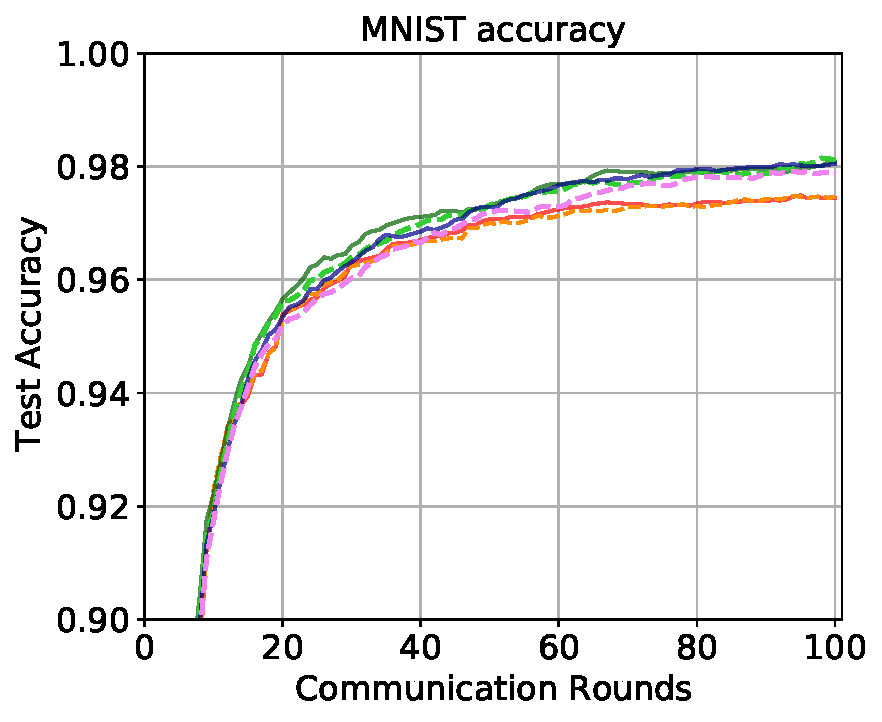
\includegraphics[width=.8\linewidth]{mnist_0.3.pdf}
  \label{fig:sub-first}
\end{subfigure}
\begin{subfigure}{.5\textwidth}
  \centering
  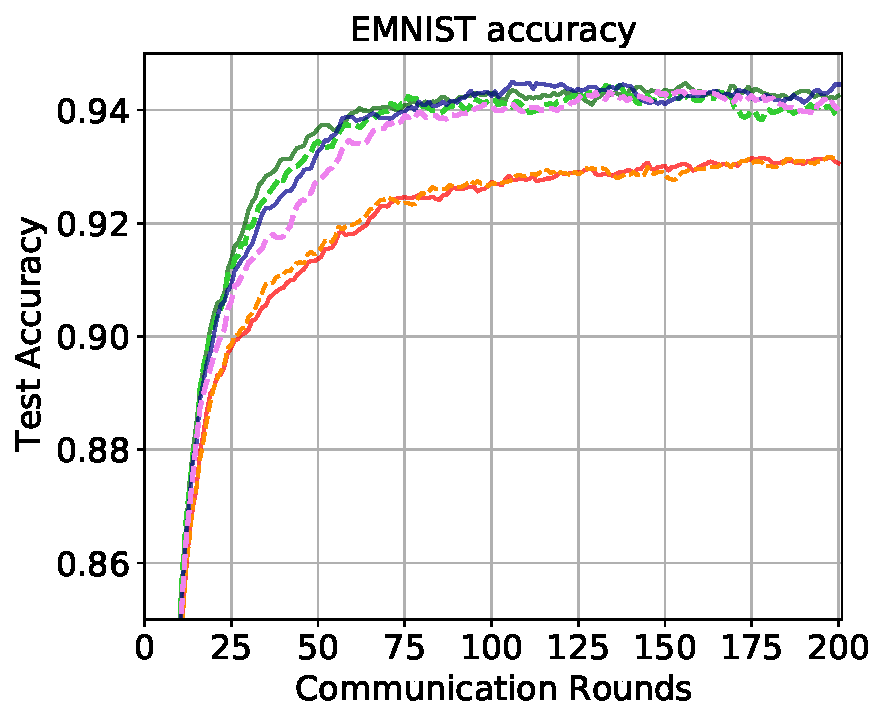
\includegraphics[width=.8\linewidth]{emnit_0.3.pdf}
  \label{fig:sub-second}
\end{subfigure}
\begin{subfigure}{.5\textwidth}
  \centering
  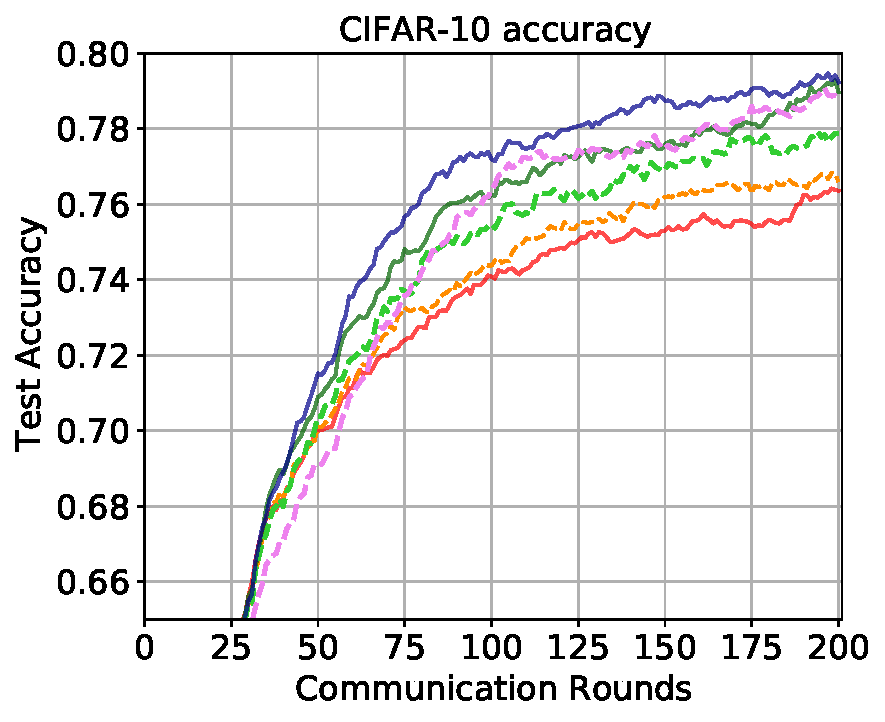
\includegraphics[width=.8\linewidth]{cifar10_0.3.pdf}
  \label{fig:sub-third}
\end{subfigure}
\begin{subfigure}{.5\textwidth}
  \centering
  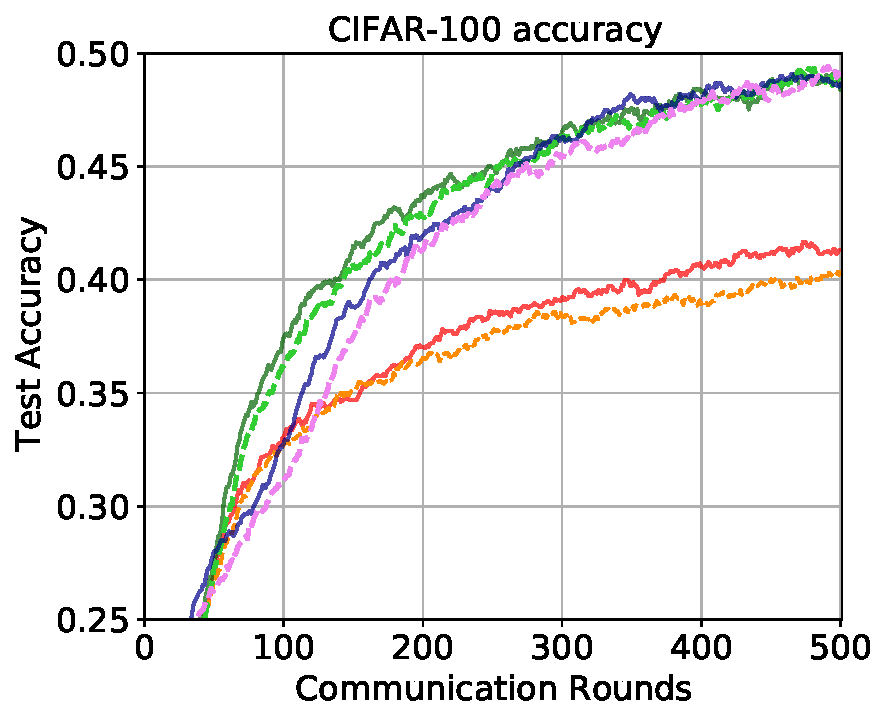
\includegraphics[width=.8\linewidth]{cifar100_0.3.pdf}
  \label{fig:sub-fourth}
\end{subfigure}
\begin{subfigure}{1\textwidth}
  \centering
  \includegraphics[width=1\linewidth]{legend.pdf}
  \label{fig:sub-Fifth}
\end{subfigure}
\caption{Classification accuracy performance evaluated in MNIST, EMNIST-L, CIFAR-10, CIFAR-100 dataset settings (10\% participation rate and Dirichlet (.3)).}
\label{fig:accuracy}
\end{figure}

\begin{figure}[ht!]
  \centering  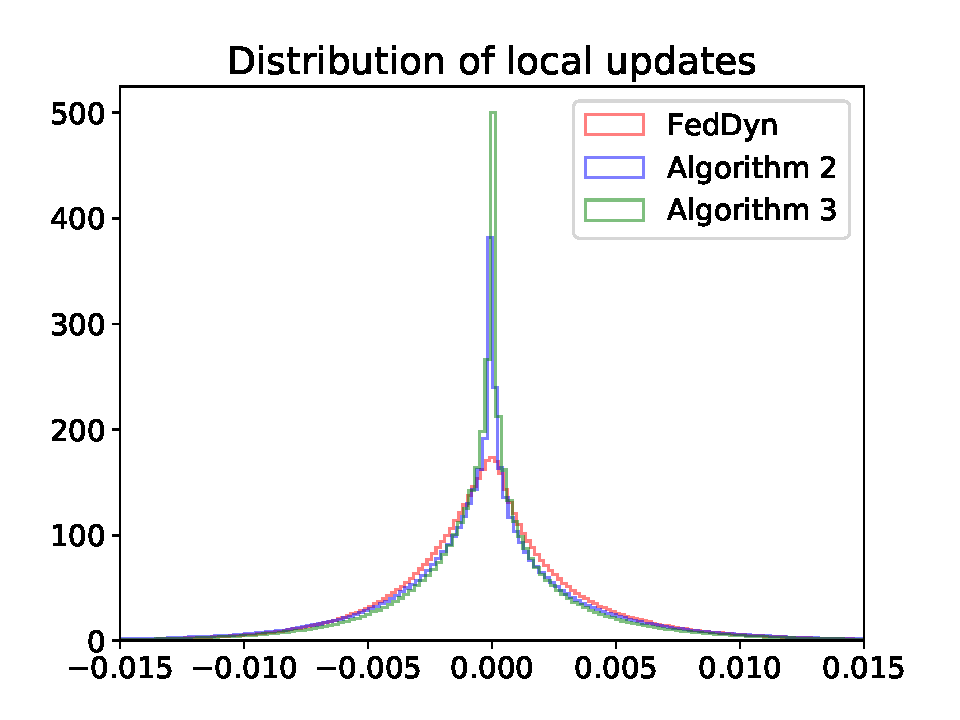
\includegraphics[width=.5\linewidth]{Distribution.pdf}  
  \caption{Comparison of distributions of transmitted local updates $\Delta_k^t = \theta_k^t - \theta^{t-1}$ (10\% participation rate and Dirichlet (.3)) for CIFAR-10.}
  \label{fig:delta_histogram}
\end{figure}

Tables~\ref{tab:entropy} and \ref{tab:100entropy} report the Shannon entropy of transmitted bits for the baseline methods with/without FedElasticNet. The communication costs of baseline methods are effectively improved by the FedElasticNet approach. Algorithms~\ref{algo:fedavg},~\ref{algo:SCAFFOLD}, and~\ref{algo:feddyn} reduce the entropy compared to the their baseline methods. We note that FedElasticNet integrated with FedDyn (Algorithm~\ref{algo:feddyn}) achieves the minimum entropy, i.e., the minimum communication cost. 

For FedDyn, we evaluate the Shannon entropy values for two cases: ({\romannumeral 1}) transmit the updated local models $\theta_k^t$ as in~\citet{Acar2021federated} and ({\romannumeral 2}) transmit the local updates $\Delta_k^t = \theta_k^t - \theta^{t-1}$ as in Algorithm~\ref{algo:feddyn}. We observe that transmitting the local updates $\Delta_k^t$ instead of the local models $\theta_k^t$ can reduce the Shannon entropy significantly. Hence, it is beneficial to transmit the local updates $\Delta_k^t$ even for FedDyn if it adopts an additional compression scheme. The numbers of nonzero elements for two cases (i.e., $\theta_k^t$ and $\Delta_k^t$) are the same for FedDyn. 

Fig.~\ref{fig:accuracy} shows that the FedElasticNet maintains the classification accuracy or incurs marginal degradation. We observe a classification gap between FedProx and Algorithm~\ref{algo:fedavg} for CIFAR-10 and CIFAR-100. However, the classification accuracies of FedDyn and Algorithm~\ref{algo:feddyn} are almost identical in the converged regime. 


In particular, Algorithm~\ref{algo:feddyn} significantly reduces the Shannon entropy, which can be explained by Fig~\ref{fig:delta_histogram}. Fig~\ref{fig:delta_histogram} compares the distributions of the transmitted local updates $\Delta_k^t$ for FedDyn, Algorithm~\ref{algo:SCAFFOLD}, and Algorithm~\ref{algo:feddyn}. Because of the $\ell_1$-norm penalty on the local updates, Algorithm~\ref{algo:feddyn} makes sparser local updates than FedDyn. The local updates of FedDyn can be modeled by the Gaussian distribution, and the local updates of FedElasticNet can be modeled by the non-Gaussian distribution (similar to the Laplacian distribution). It is well-known that the Gaussian distribution maximizes the entropy for a given variance in information theory~\cite{Cover2006elements}. Hence, FedElasticNet can reduce the entropy by transforming the Gaussian distribution into the non-Gaussian one. 




% Table~\ref{tab:nonzero} reports the number of non-zero elements of the baseline methods and FedElasticNet. Basically, the communication costs per round of FedProx and FedDyn are the same; however, FedDyn effectively resolves the client drift problem as shown in Fig.~\ref{fig:accuracy}. SCAFFOLD suffers from the highest communication cost because of the control variates. The proposed FedElasticNet integrations (Algorithms~\ref{algo:fedavg}, ~\ref{algo:SCAFFOLD}, and~\ref{algo:feddyn}) can effectively sparsify the transmitted local updates, which enhances communication efficiency. Furt Fig.~\ref{fig:accuracy} shows that FedElasticNet maintains the classification accuracy of its baseline method. 



% \paragraph{Reduced non-zero elements}
% We report the number of cumulative non-zero elements transmitted in Table\ref{tab:nonzero}. To fairly compare the communication cost reduction due to the addition of the elastic net regularization term, the SCAFFOLD and proposed 2 algorithms in Table\ref{tab:nonzero} ignore the transmission of the control variate and count only the model transmission. The proposed 1 and 2 algorithms showed the most significant reduction in communication cost in the 0.3 mnist environments. They achieved the same performance with the number of non-zero elements of 31.97\% and 71.87\% compared to the existing base algorithm.
% The proposed 3 algorithms showed the most significant reduction in communication cost in the Dirichlet(.6) EMNIST-L dataset setting with a client participation rate of 10\% and achieved the same performance with the number of non-zero elements of 11.14\% compared to the base algorithm. The cumulative number of non-zero elements in the all round are detailed in table\ref{tab:nonzero}.

% \paragraph{Reduced the differential entropy}
% We report the cumulative differential entropy in Table\ref{tab:entropy}. Our proposed 1 algorithm shows the same performance as the FedProx algorithm by transmitting only 18.23\% of the cumulative entropy of the baseline algorithm in the Dirichlet(.6) MNIST dataset setting with a client participation rate of 10\%. In the EMNIST-L dataset, only 25.26\% of the baseline algorithm cumulative entropy is transmitted at the 10\% client participation rate Dirichlet (.6) setting. In both the CIFAR-10 and CIFAR-100 datasets, the lowest cumulative entropy is transmitted at the 10\% participation rate Dirichlet (.3) setting, and 33.99\% and 25.27\% of cumulative entropy are transmitted compared to the baseline algorithm of each dataset. Only 62.450\% of the baseline algorithm cumulative entropy for the Shakespeare dataset is transmitted for the 10\% participation rate IID setting.

% Our proposed 2 algorithm shows the same performance as the SCAFFOLD algorithm by transmitting only 25.05\% of the cumulative entropy of the baseline algorithm in the Dirichlet(.3) MNIST dataset setting with a client participation rate of 10\%. In the EMNIST-L dataset, only 43.90\% of the baseline algorithm cumulative entropy is transmitted at the 10\% client participation rate Dirichlet (.3) setting. In both the CIFAR-10 and CIFAR-100 datasets, the lowest cumulative entropy is transmitted at the 10\% participation rate Dirichlet (.3) setting, and 72.74\% and 49.72\% of cumulative entropy are transmitted compared to the baseline algorithm of each dataset. Only 43.51\% of the baseline algorithm cumulative entropy for the Shakespeare dataset is transmitted for the 10\% participation rate IID setting.

% Our proposed 3 algorithm shows the same performance as the FedDyn algorithm by transmitting only 6.32\% of the cumulative entropy of the baseline algorithm in the Dirichlet(.3) MNIST dataset setting with a client participation rate of 10\%. In the EMNIST-L dataset, only 12.76\% of the baseline algorithm cumulative entropy is transmitted at the 10\% client participation rate Dirichlet (.6) setting. In both the CIFAR-10 and CIFAR-100 datasets, the lowest cumulative entropy is transmitted at the 10\% participation rate Dirichlet (.3) setting, and 18.03\% and 19.74\% of cumulative entropy are transmitted compared to the baseline algorithm of each dataset. Only 39.12\% of the baseline algorithm cumulative entropy for the Shakespeare dataset is transmitted for the 10\% participation rate IID setting. The cumulative entropy values in the all round are detailed in table\ref{tab:entropy}.

\section{Conclusion}

We proposed FedElasticNet, a general framework to improve communication efficiency and resolve the client drift problem simultaneously. We introduce two types of penalty terms on the local model updates by repurposing the classical elastic net. The $\ell_1$-norm regularizer sparsifies the local model updates, which reduces the communication cost. The $\ell_2$-norm regularizer limits the impact of variable local updates to resolve the client drift problem. Importantly, our framework can be integrated with prior FL techniques so as to simultaneously resolve the communication cost problem and the client drift problem. By integrating FedElasticNet with FedDyn, we can achieve the best communication efficiency while maintaining classification accuracy for heterogeneous datasets. 



% The feddynsd algorithm we proposed has the same global model accuracy as the feddyn algorithm, and the server and client communicate using the entropy of at least  6.32\% of the cumulative entropy of the feddyn algorithm. These results dramatically improve communication efficiency while resolving 'client drift' suggested by \citep{Karimireddy2020scaffold}.
% Although there have been many attempts to solve the problems of 'client drift' and communication efficiency respectively in previous FL studies, it was our first attempt to deal with both problems simultaneously. In addition, we propose fedproxsd, fedproxela, and scaffoldsd algorithms by applying the method used to increase communication efficiency in the feddynsd algorithm to other federated learning algorithms. These three algorithms use less entropy than the baseline algorithm to produce the same performance. The applied method can be used as a generalized algorithm to increase communication efficiency.

\clearpage


% \subsubsection*{Author Contributions}
% If you'd like to, you may include  a section for author contributions as is done
% in many journals. This is optional and at the discretion of the authors.

% \subsubsection*{Acknowledgments}
% Use unnumbered third level headings for the acknowledgments. All
% acknowledgments, including those to funding agencies, go at the end of the paper.


\bibliography{mybib}
\bibliographystyle{iclr2023_conference}
\clearpage

\appendix
\section{Appendix}
\subsection{Experiment Details}
We provide the details of our experiments. We select the datasets for our experiments, including those used in prior work on federated learning~\citep{McMahan2017communication,Li2020federated,Acar2021federated}. To fairly compare the non-IID environments, the datasets and the experimental environments are the same as those of \citet{Acar2021federated}.
\paragraph{Hyperparameters.}
We describe the hyperparameters used in our experiments in Section~\ref{section:experiments}. We perform a grid search to find the best $\lambda_{1}$ and $\epsilon$ used in the proposed algorithms. Each hyperparameter was selected to double the value as the performance improved. We use the same $\lambda_{2}$ as in \citet{Acar2021federated}. SCAFFOLD has the same local epoch and batch size as other algorithms, and SCAFFOLD is not included in Table 4 because other hyperparameters are not required. Table~\ref{tab:hyperparameter} shows the hyperparameters used in our experiments.

% lambda_1, epsilon은 optimize한 값임; lambda_2는 FedDyn 논문의 값을 그대로 사용
\begin{table}[ht!]
\centering
\resizebox{8cm}{!}{%
\begin{tabular}{|c|cccc|}
\hline
\textbf{Dataset} &
  \multicolumn{1}{c|}{\textbf{Algorithm}} &
  \multicolumn{1}{c|}{\textbf{$\lambda_{1}$}} &
  \multicolumn{1}{c|}{\textbf{$\lambda_{2}$}} &
  \textbf{$\epsilon$} \\ \hline
\multirow{5}{*}{\textbf{CIFAR-10}}    & FedProx     & -         & $10^{-4}$         & -                 \\
& Algorithm 1 & $10^{-6}$ & $10^{-4}$         & $10^{-3}$         \\
& Algorithm 2 & $10^{-4}$ & 0                 & $10^{-4}$         \\
                                      & FedDyn      & -         & $10^{-2}$         & -                 \\
                                      & Algorithm 3 & $10^{-4}$ & $10^{-2}$         & $5\times 10^{-3}$ \\ \hline
\multirow{5}{*}{\textbf{CIFAR-100}}   & FedProx     & -         & $10^{-4}$         & -     \\
                                      & Algorithm 1 & $10^{-6}$ & $10^{-4}$         & $10^{-3}$                 \\
                                      & Algorithm 2 & $10^{-4}$ & 0                 & $10^{-4}$         \\
                                      & FedDyn      & -         & $10^{-2}$         & -        \\
                                      & Algorithm 3 & $10^{-4}$ & $10^{-2}$         & $10^{-3}$                  \\ \hline
\multirow{5}{*}{\textbf{MNIST}}       & FedProx     & -         & $10^{-4}$         & -         \\
                                      & Algorithm 1 & $10^{-6}$ & $10^{-6}$         & $10^{-3}$         \\
                                      & Algorithm 2 & $10^{-4}$ & 0                 & $10^{-4}$         \\
                                      & FedDyn      & -         & $5\times 10^{-2}$ & -                 \\
                                      & Algorithm 3 & $10^{-4}$ & $5\times 10^{-2}$ & $5\times 10^{-3}$ \\ \hline
\multirow{5}{*}{\textbf{EMNIST-L}}   & FedProx     & -         & $10^{-4}$         & -                 \\
                                      & Algorithm 1 & $10^{-6}$ & $10^{-6}$         & $10^{-3}$         \\
                                      & Algorithm 2 & $10^{-4}$ & 0                 & $10^{-4}$         \\
                                      & FedDyn      & -         & $4\times 10^{-2}$ & -                 \\
                                      & Algorithm 3 & $10^{-4}$ & $4\times 10^{-2}$ & $2\times 10^{-3}$ \\ \hline
\multirow{5}{*}{\textbf{Shakespeare}} & FedProx     & -         & $10^{-4}$         & -                 \\
                                      & Algorithm 1 & $10^{-6}$ & $10^{-6}$         & $9\times 10^{-3}$ \\
                                      & Algorithm 2 & $10^{-6}$ & 0                 & $9\times 10^{-4}$ \\
                                      & FedDyn      & -         & $10^{-2}$         & -                 \\
                                      & Algorithm 3 & $10^{-6}$ & $10^{-2}$         & $10^{-2}$         \\ \hline
\end{tabular}%
}
\caption{Hyperparameters.}
\label{tab:hyperparameter}
\end{table}

% \subsection{Comparison with Full Participation and 10\% Participation }
% In Section~\ref{section:experiments}, Tables~\ref{tab:entropy} and \ref{tab:100entropy} report the Shannon entropy of transmitted bits for the baseline methods with/without FedElasticNet.
% Table~\ref{tab:entropy} is the experimental results with 10\% participation of clients, and Table~\ref{tab:100entropy} is with 100\% participation. These results show that FedElasticNet is more effective at a 100\% participation rate. In the full participation setting, FedElasticNet influence faster model convergence, significantly reducing communication costs. In~\citet{Acar2021federated} reported that FedDyn is robust in the full participation rate environment. FedElasticNet (Algorithm~\ref{algo:feddyn}) is also robust in the full participation rate environment more than others (see Fig.~\ref{fig:100peracc1} and Fig.~\ref{fig:100peracc2}). Feddyn and Algorithm~\ref{algo:feddyn}, which have a more robust convergence rate in the overall participation rate environment, can see more communication cost reduction.


\subsection{Regularizer Coefficients}

We selected $\lambda_{1}$ over $\{10^{-2}, 10^{-4}, 10^{-6}, 10^{-8} \}$ to observe the impact of $\lambda_1$ on the classification accuracy. We prefer a larger $\lambda_1$ to enhance communication efficiency unless the $\ell_1$-norm regularizer does not degrade the classification accuracy. Figures~\ref{fig:algo1 lambda1}, \ref{fig:algo2 lambda1}, and \ref{fig:algo3 lambda1} show the classification accuracy depending on $\lambda_{1}$ in the CIFAR-10 dataset with 10\% participation rate and Dirichlet (.3). The unit of the cumulative number of elements is $10^{7}$.

In Algorithm~\ref{algo:fedavg}, we selected $\lambda_1 = 10^{-6}$ to avoid a degradation of classification accuracy (see Fig.~\ref{fig:algo1 lambda1}) and maximize the sparsity of local updates. In this way, we selected the coefficient values $\lambda_1$ (See Fig.\ref{fig:algo2 lambda1} for Algorithm~\ref{algo:SCAFFOLD} and \ref{fig:algo3 lambda1} and Algorithm~\ref{algo:feddyn}).

\begin{figure}[ht!]
\begin{subfigure}{.5\textwidth}
  \centering
  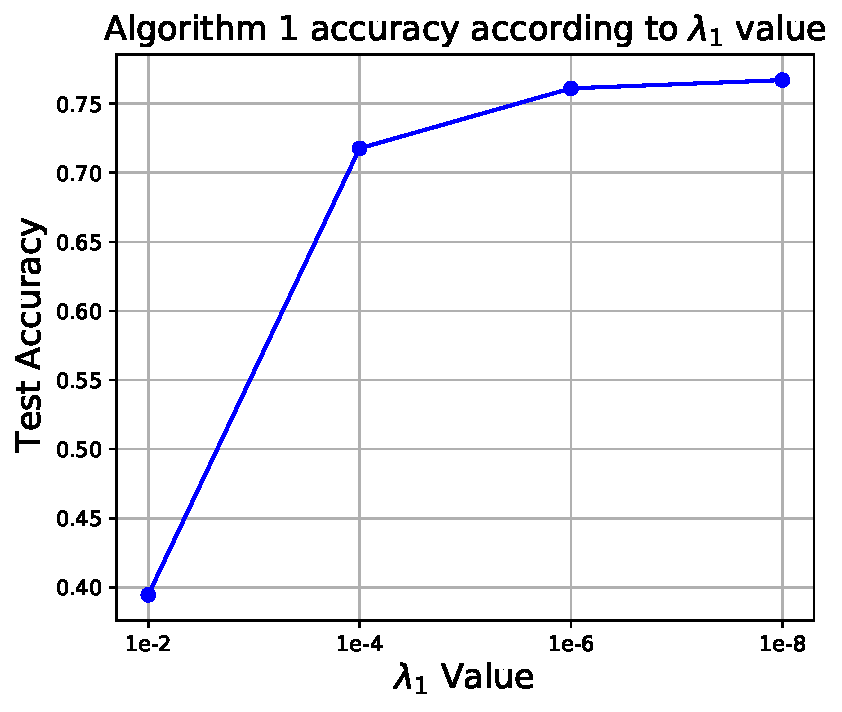
\includegraphics[width=.8\linewidth]{textfigure/algo1acc.pdf}
  \label{fig:sub31}
\end{subfigure}
\begin{subfigure}{.5\textwidth}
  \centering
  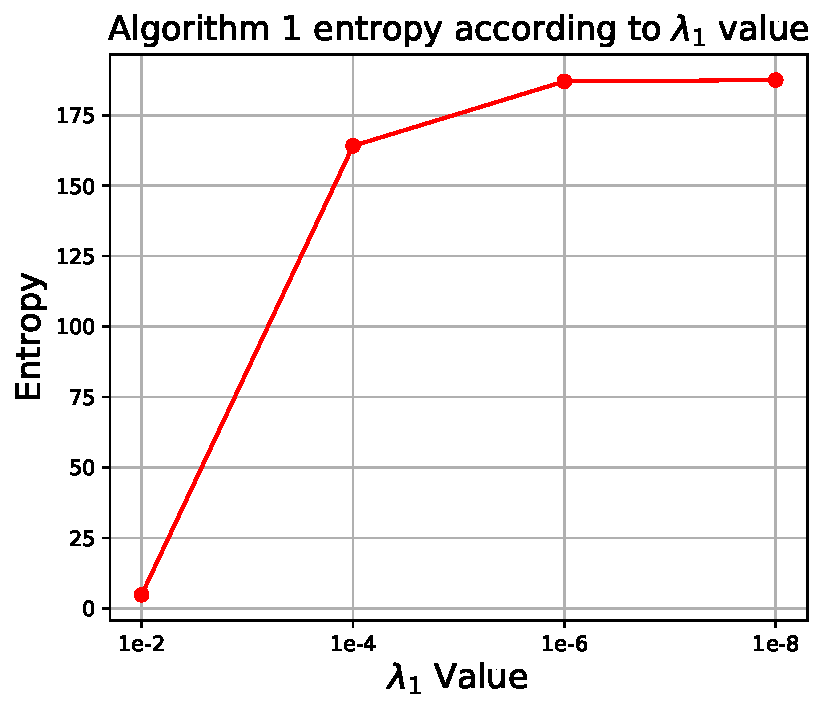
\includegraphics[width=.8\linewidth]{textfigure/algo1entropy.pdf}
  \label{fig:sub32}
\end{subfigure}
\begin{subfigure}{1\textwidth}
  \centering
  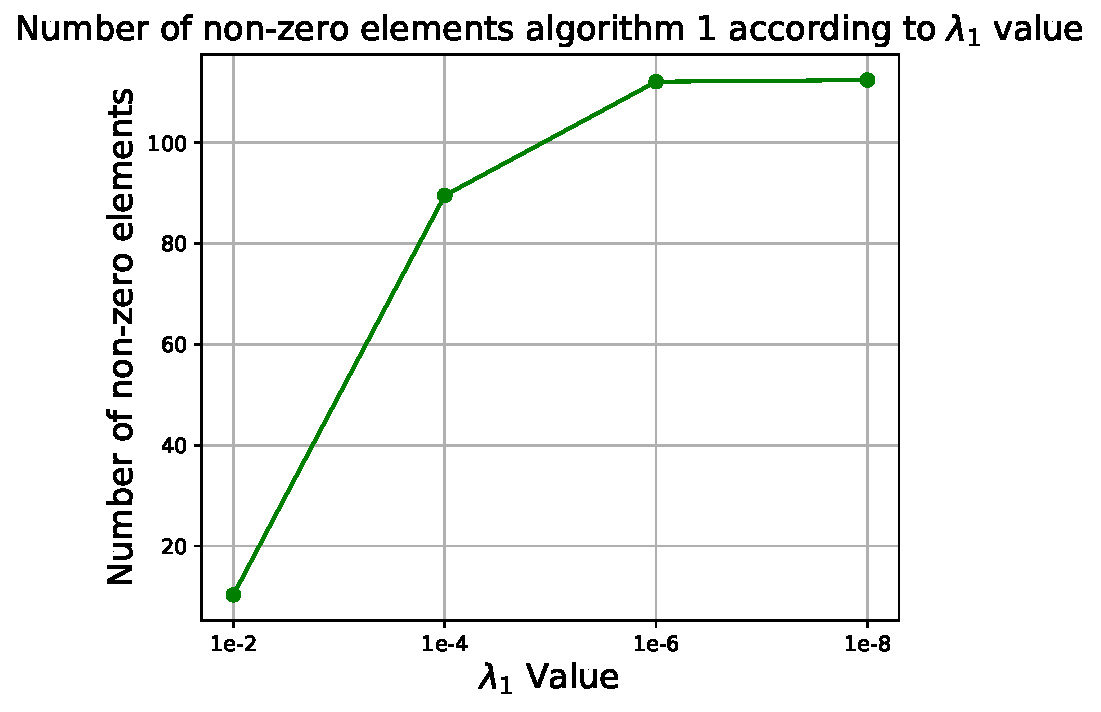
\includegraphics[width=.6\linewidth]{textfigure/algo1nonzero.pdf}
  \label{fig:sub33}
\end{subfigure}
\caption{Classification accuracy and sparsity of local updates depending on $\lambda_{1}$ (Algorithm~\ref{algo:fedavg}).}
\label{fig:algo1 lambda1}
\end{figure}


\begin{figure}[ht!]
\begin{subfigure}{.5\textwidth}
  \centering
  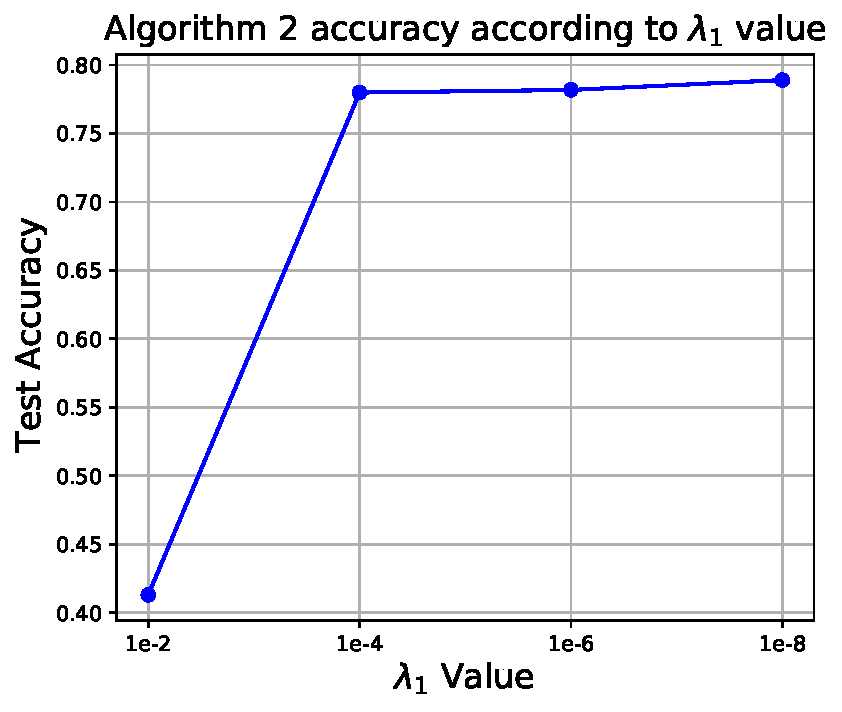
\includegraphics[width=.8\linewidth]{textfigure/algo2acc.pdf}
  \label{fig:sub41}
\end{subfigure}
\begin{subfigure}{.5\textwidth}
  \centering
  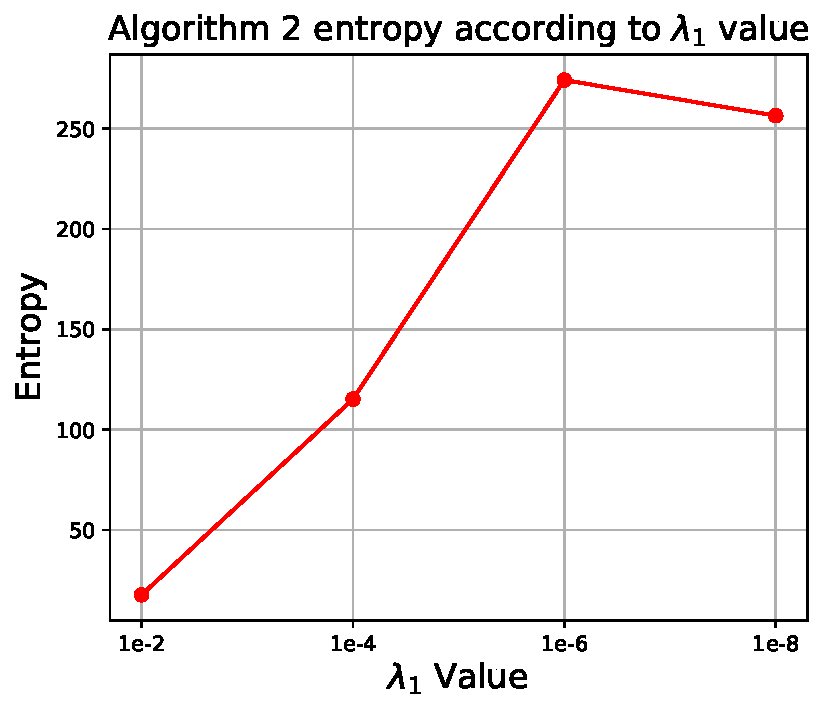
\includegraphics[width=.8\linewidth]{textfigure/algo2entropy.pdf}
  \label{fig:sub42}
\end{subfigure}
\begin{subfigure}{1\textwidth}
  \centering
  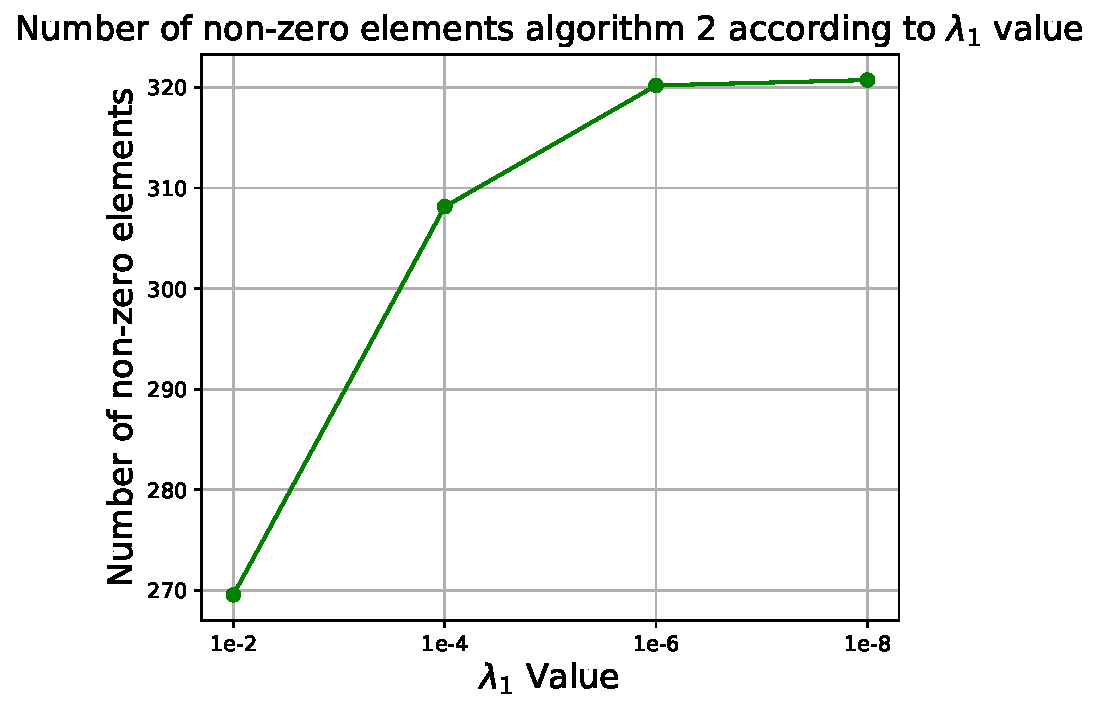
\includegraphics[width=.6\linewidth]{textfigure/algo2nonzero.pdf}
  \label{fig:sub43}
\end{subfigure}
\caption{Classification accuracy and sparsity of local updates depending on $\lambda_{1}$ (Algorithm~\ref{algo:SCAFFOLD}).}
\label{fig:algo2 lambda1}
\end{figure}

\begin{figure}[ht!]
\begin{subfigure}{.5\textwidth}
  \centering
  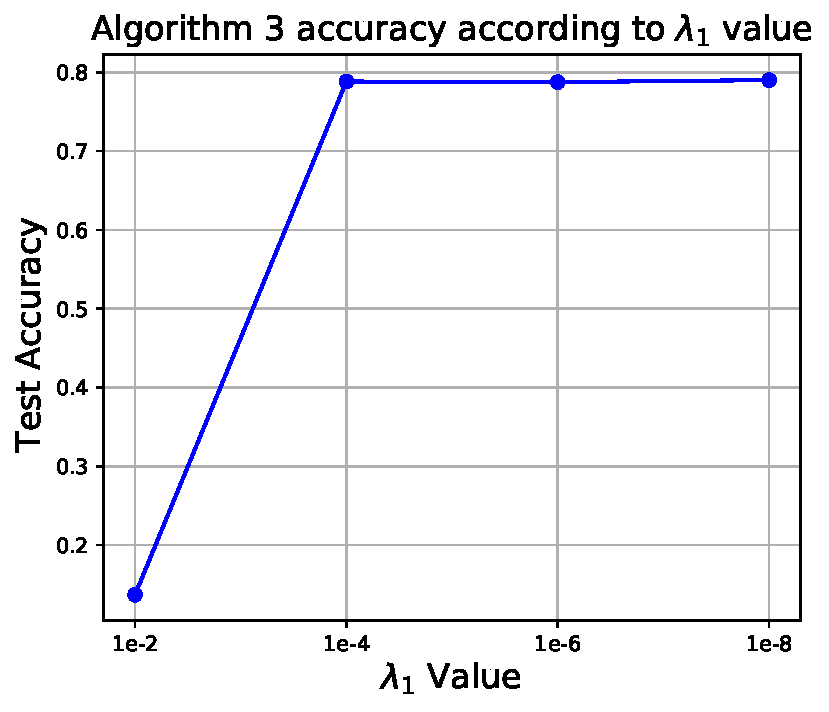
\includegraphics[width=.8\linewidth]{textfigure/algo3acc.pdf}
  \label{fig:sub51}
\end{subfigure}
\begin{subfigure}{.5\textwidth}
  \centering
  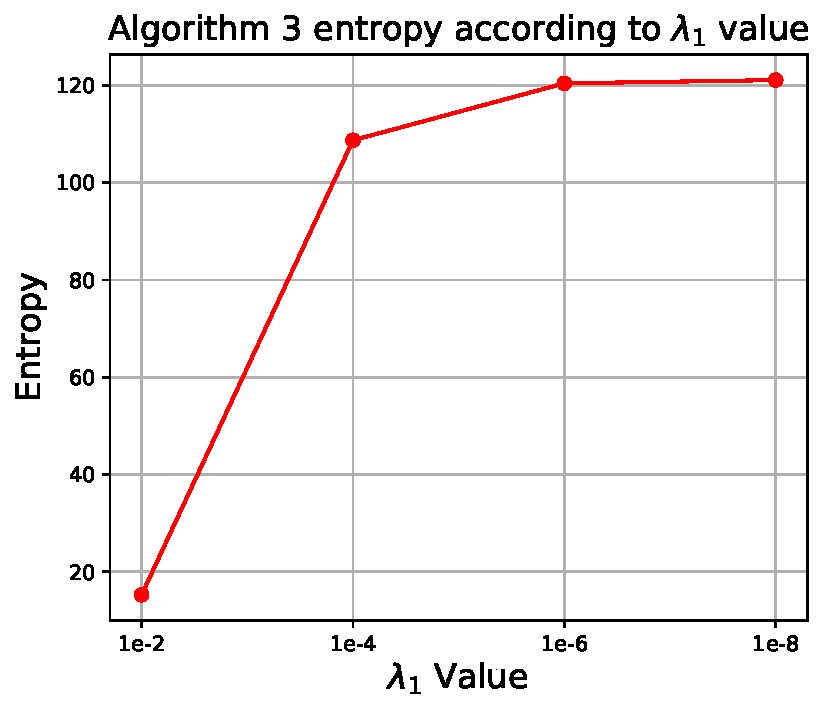
\includegraphics[width=.8\linewidth]{textfigure/algo3entropy.pdf}
  \label{fig:sub52}
\end{subfigure}
\begin{subfigure}{1\textwidth}
  \centering
  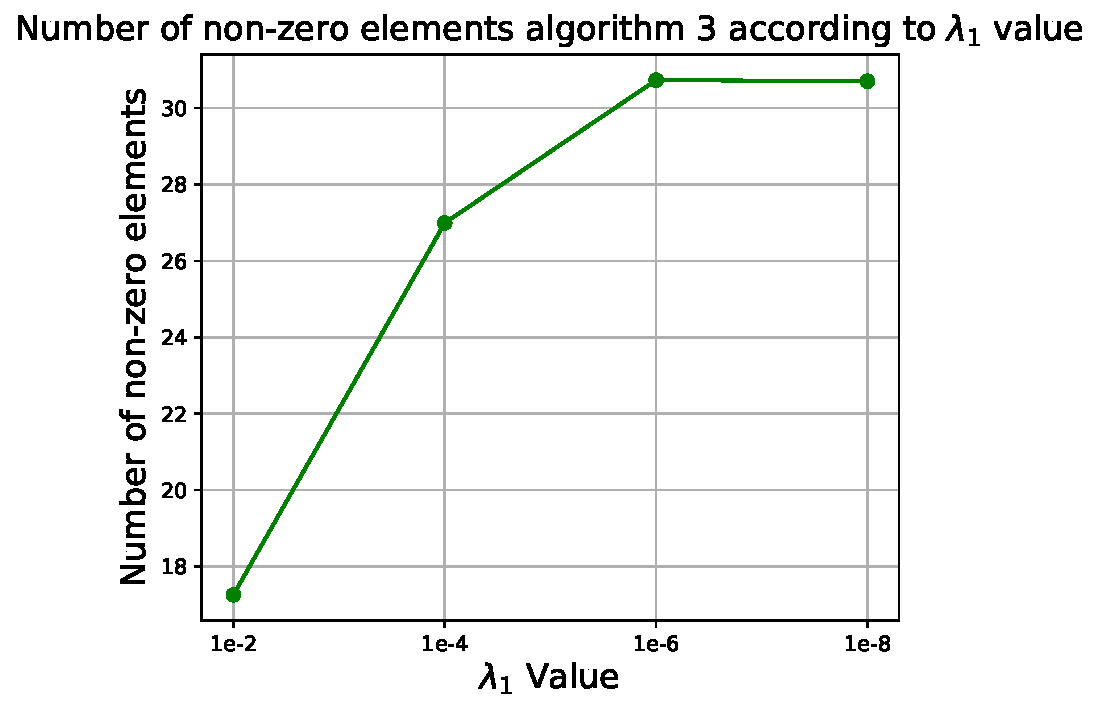
\includegraphics[width=.6\linewidth]{textfigure/algo3nonzero.pdf}
  \label{fig:sub53}
\end{subfigure}
\caption{Classification accuracy and sparsity of local updates depending on $\lambda_{1}$ (Algorithm~\ref{algo:feddyn}).}
\label{fig:algo3 lambda1}
\end{figure}

\clearpage

\subsection{Empirical Results of Classification Accuracy}

\begin{figure}[ht!]
\begin{subfigure}{.5\textwidth}
  \centering
  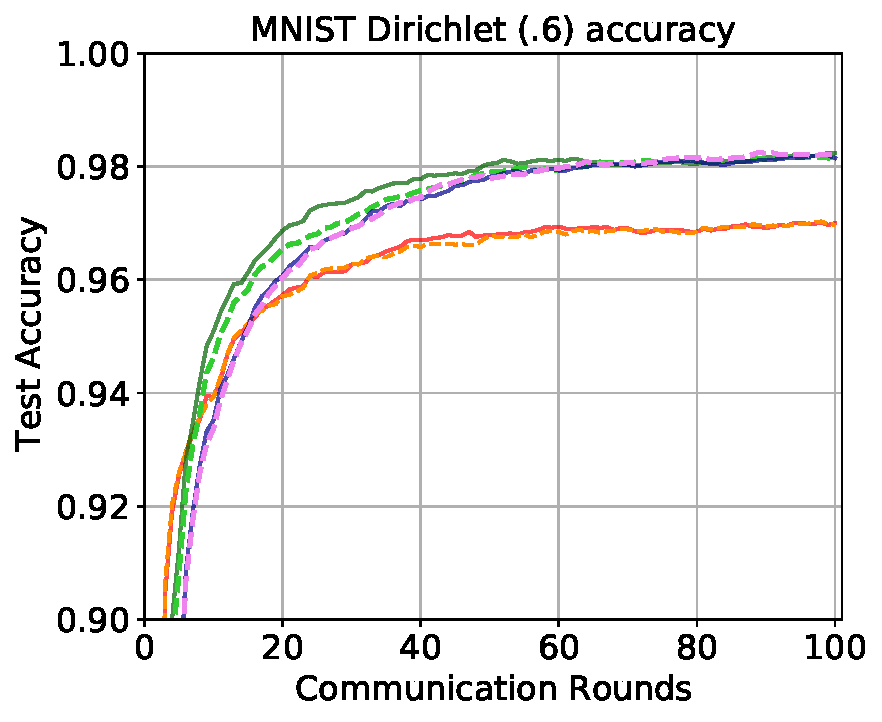
\includegraphics[width=.8\linewidth]{textfigure/mnist_0.6.pdf}
  \label{fig:sub1-first}
\end{subfigure}
\begin{subfigure}{.5\textwidth}
  \centering
  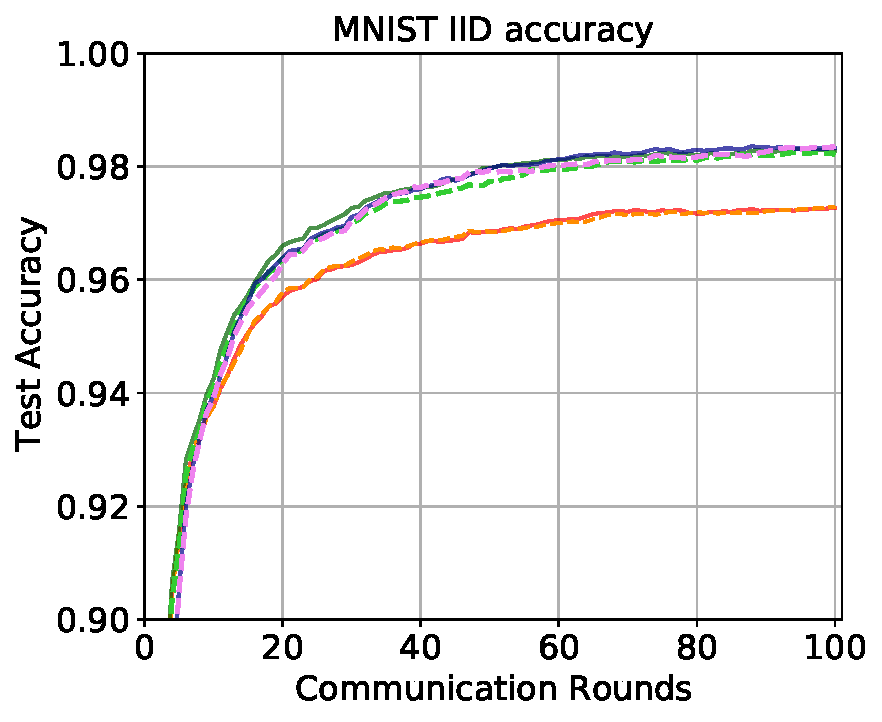
\includegraphics[width=.8\linewidth]{textfigure/mnist_iid.pdf}
  \label{fig:sub1-second}
\end{subfigure}
\begin{subfigure}{.5\textwidth}
  \centering
  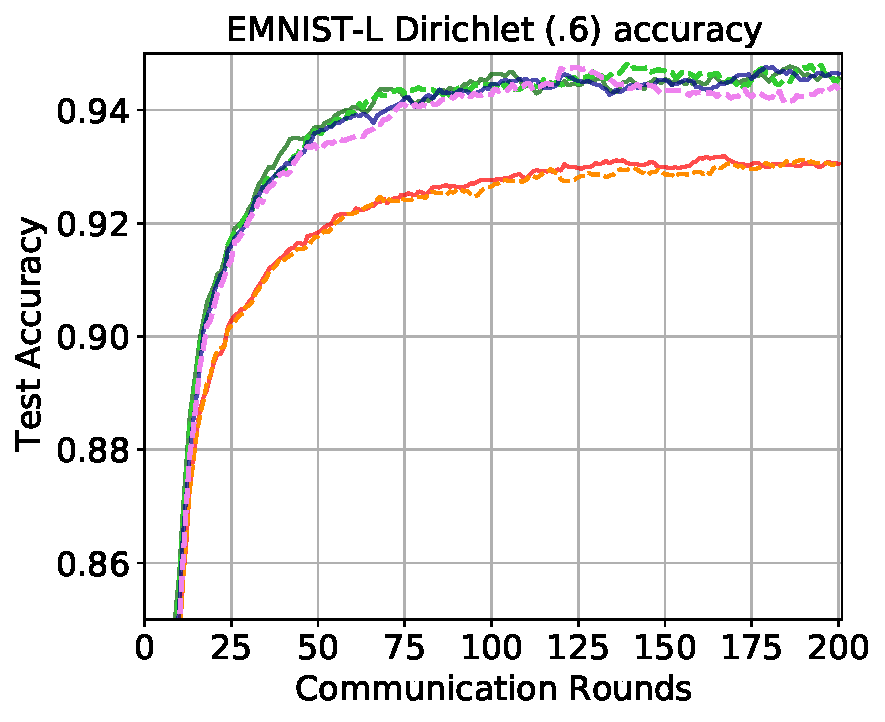
\includegraphics[width=.8\linewidth]{textfigure/emnist_0.6.pdf}
  \label{fig:sub1-third}
\end{subfigure}
\begin{subfigure}{.5\textwidth}
  \centering
  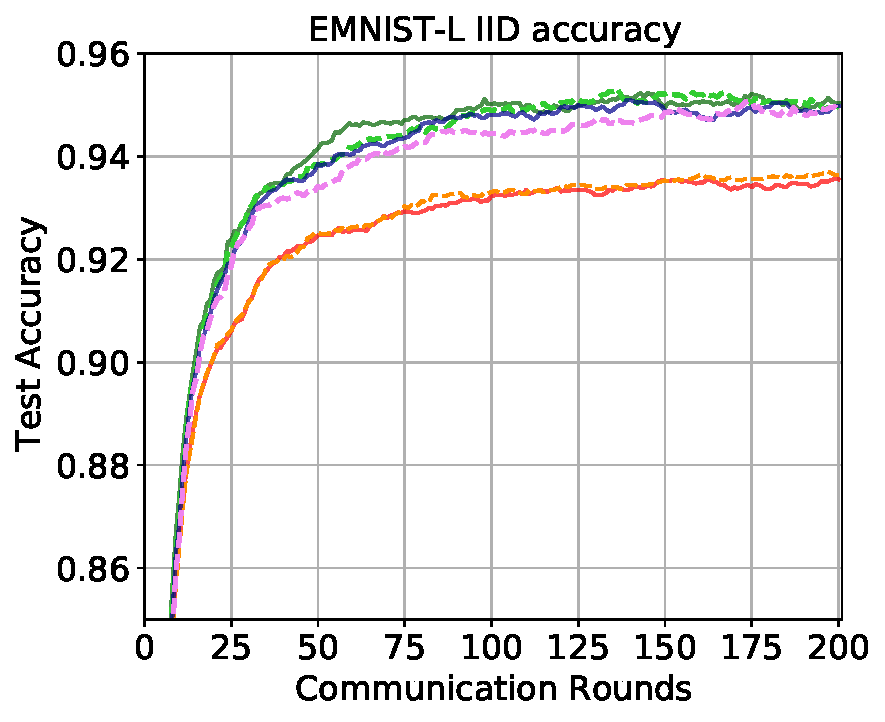
\includegraphics[width=.8\linewidth]{textfigure/emnist_iid.pdf}
  \label{fig:sub1-fourth}
\end{subfigure}
\begin{subfigure}{.5\textwidth}
  \centering
  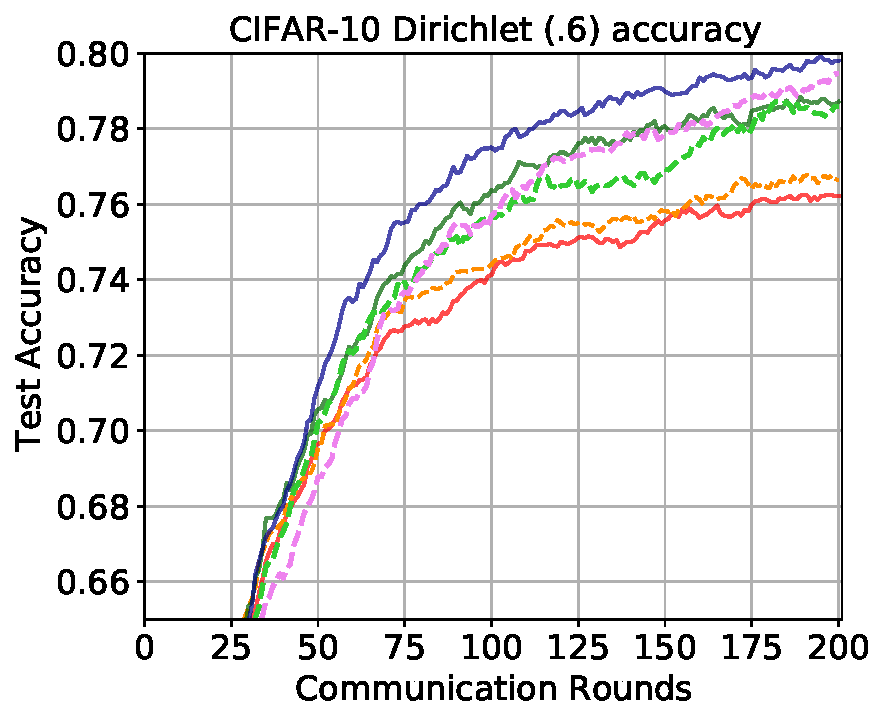
\includegraphics[width=.8\linewidth]{textfigure/cifar10_0.6.pdf}
  \label{fig:sub1-Fifth}
\end{subfigure}
\begin{subfigure}{.5\textwidth}
  \centering
  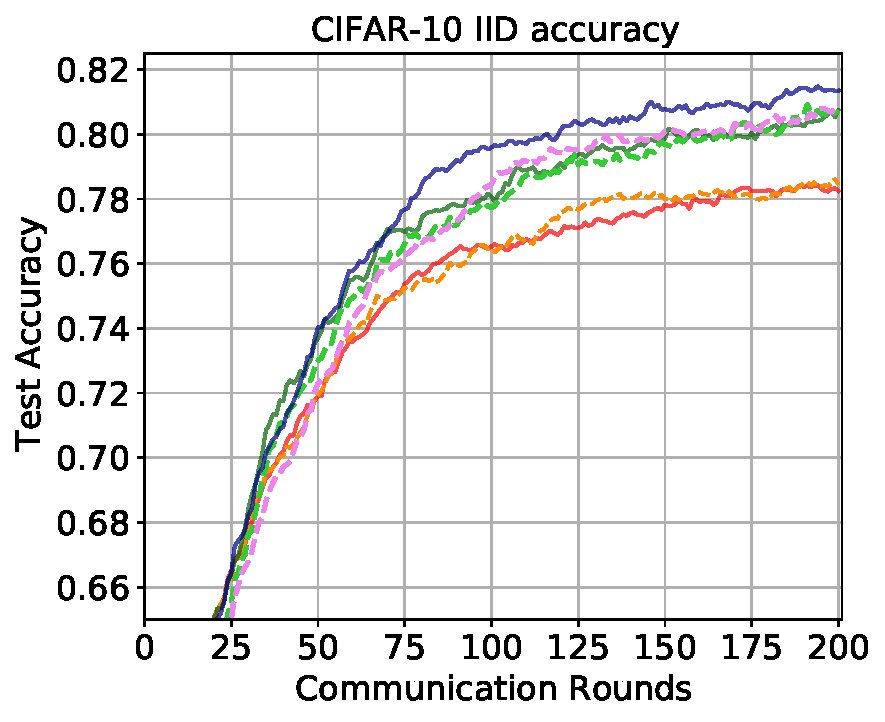
\includegraphics[width=.8\linewidth]{textfigure/cifar10_iid.pdf}
  \label{fig:sub1-sixth}
\end{subfigure}
\begin{subfigure}{.5\textwidth}
  \centering
  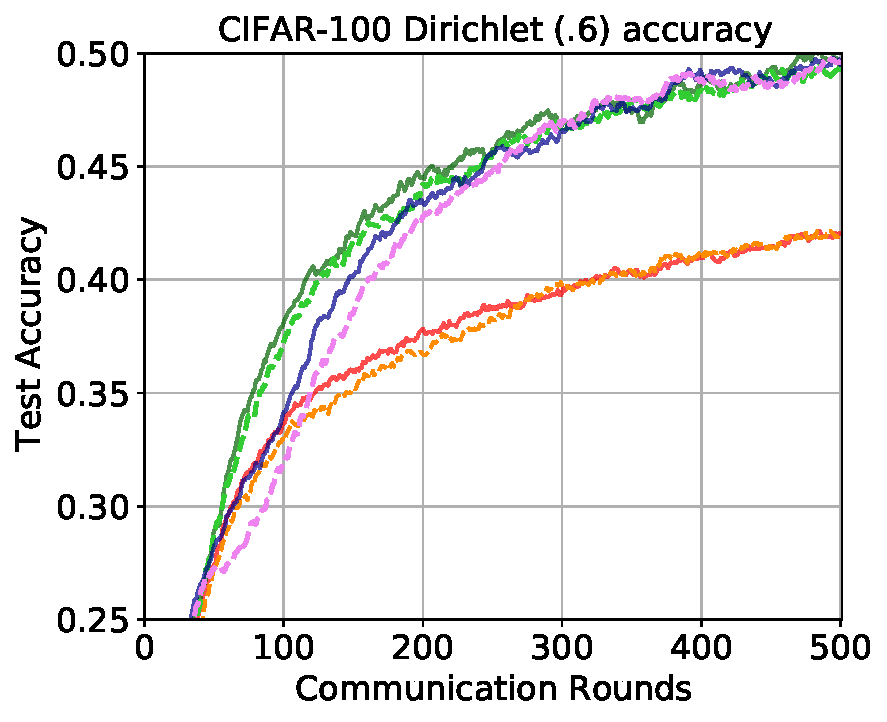
\includegraphics[width=.8\linewidth]{textfigure/cifar100_0.6.pdf}
  \label{fig:sub1-seventh}
\end{subfigure}
\begin{subfigure}{.5\textwidth}
  \centering
  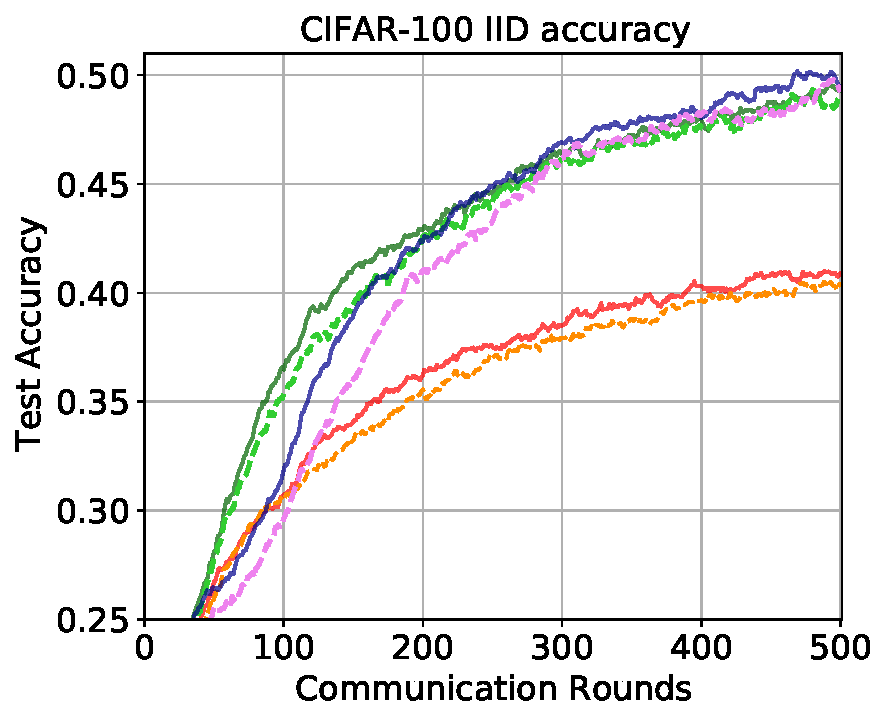
\includegraphics[width=.8\linewidth]{textfigure/cifar100_iid.pdf}
  \label{fig:sub1-eighth}
\end{subfigure}
\begin{subfigure}{1\textwidth}
  \centering
  \includegraphics[width=1\linewidth]{textfigure/legend.pdf}
  \label{fig:sub1-11}
\end{subfigure}
\caption{Classification accuracy performance evaluated in MNIST, EMNIST-L, CIFAR-10, and CIFAR-100 datasets (10\% participation rate). }
\label{fig:maintextacc}
\end{figure}

\begin{figure}[ht!]
\begin{subfigure}{.5\textwidth}
  \centering
  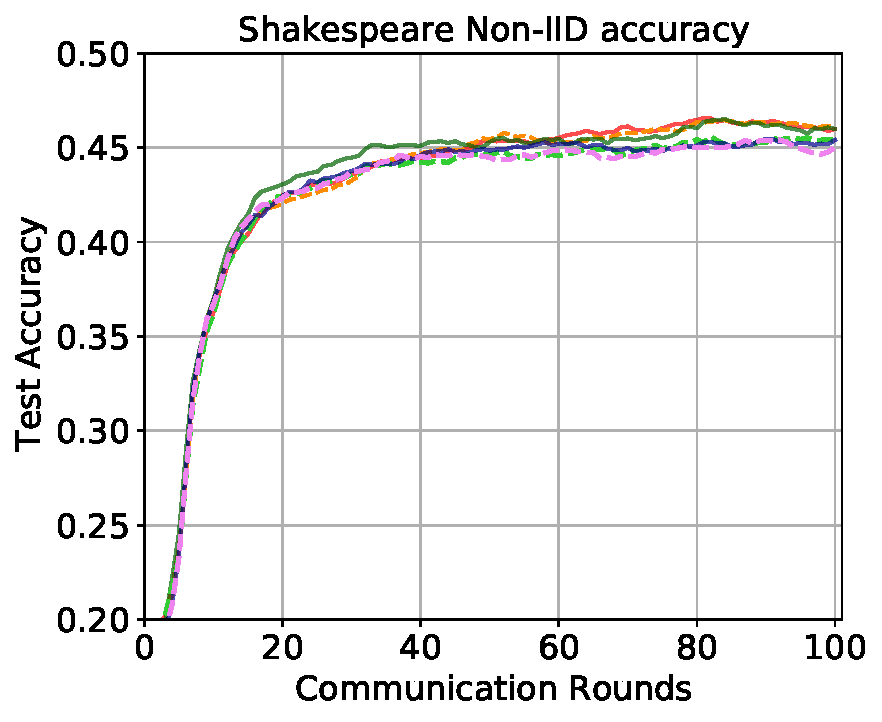
\includegraphics[width=.8\linewidth]{textfigure/Shakespeare_noniid.pdf}
  \label{fig:sub-1}
  \caption{10\% participation rate}
\end{subfigure}
\begin{subfigure}{.5\textwidth}
  \centering
  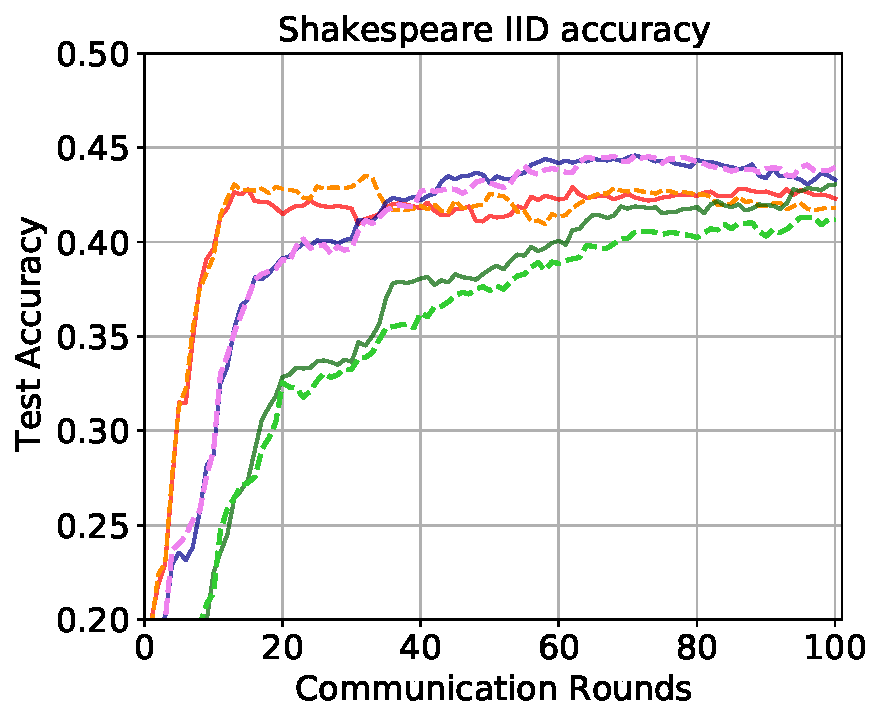
\includegraphics[width=.8\linewidth]{textfigure/Shakespeare_iid.pdf}
  \label{fig:sub-2}
  \caption{10\% participation rate}
\end{subfigure}
\begin{subfigure}{.5\textwidth}
  \centering
  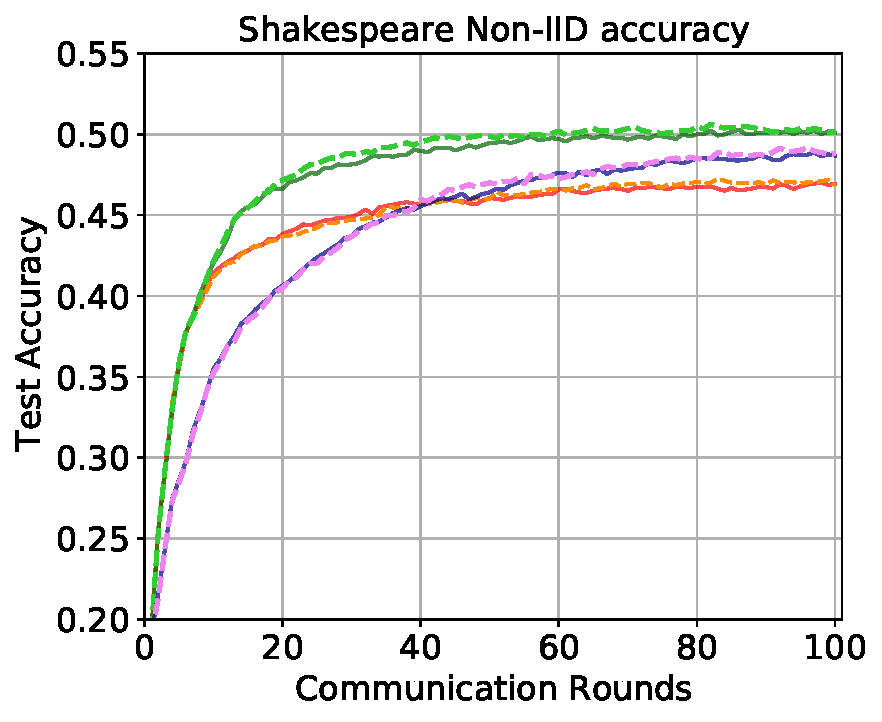
\includegraphics[width=.8\linewidth]{100perfig/Shakespeare_noniid.pdf}
  \label{fig:sub-4}
  \caption{100\% participation rate}
\end{subfigure}
\begin{subfigure}{.5\textwidth}
  \centering
  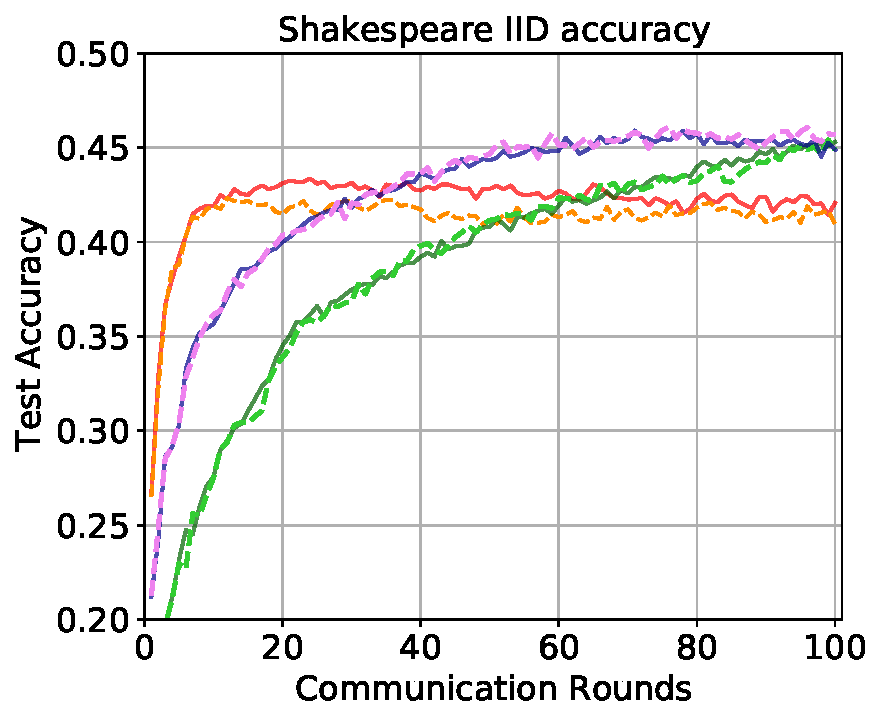
\includegraphics[width=.8\linewidth]{100perfig/Shakespeare_iid.pdf}
  \label{fig:sub-5}
  \caption{100\% participation rate}
\end{subfigure}
\begin{subfigure}{1\textwidth}
  \centering
  \includegraphics[width=1\linewidth]{textfigure/legend.pdf}
  \label{fig:sub-3}
\end{subfigure}
\caption{Classification accuracy performance evaluated in IID Shakespeare and Non-IID Shakespeare datasets.}
\label{fig:Shakespeare 10 accuracy}
\end{figure}

\begin{figure}[ht!]
\begin{subfigure}{.5\textwidth}
  \centering
  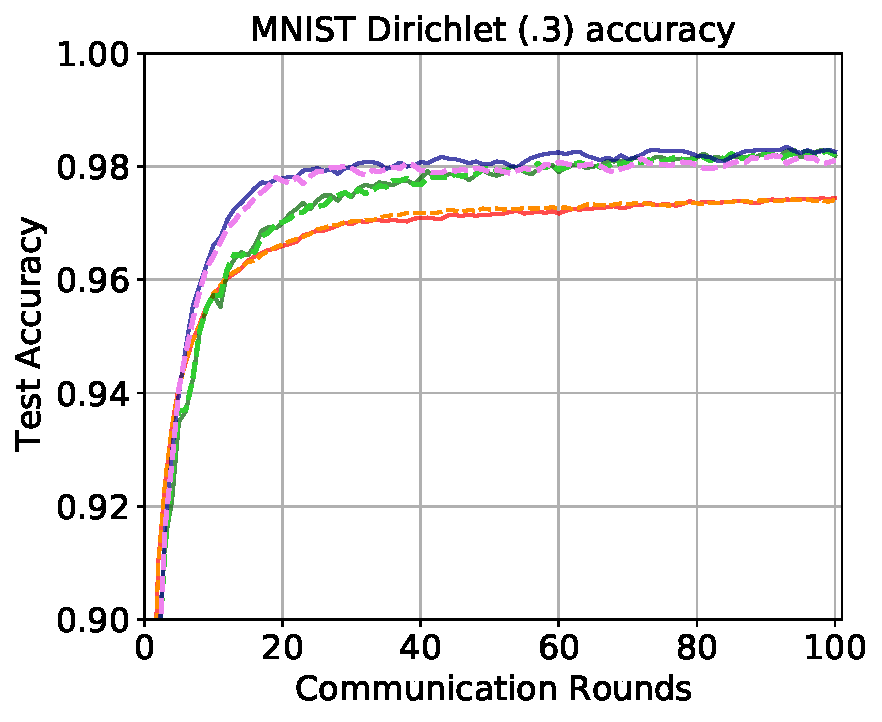
\includegraphics[width=.8\linewidth]{100perfig/mnist_0.3.pdf}
  \label{fig:sub11}
\end{subfigure}
\begin{subfigure}{.5\textwidth}
  \centering
  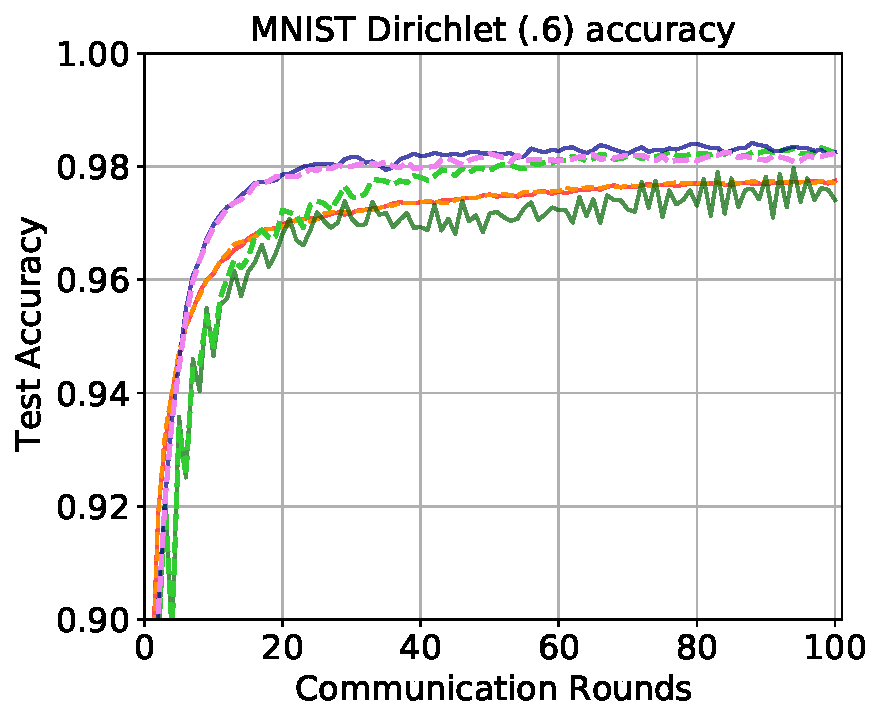
\includegraphics[width=.8\linewidth]{100perfig/mnist_0.6.pdf}
  \label{fig:sub12}
\end{subfigure}
\begin{subfigure}{.5\textwidth}
  \centering
  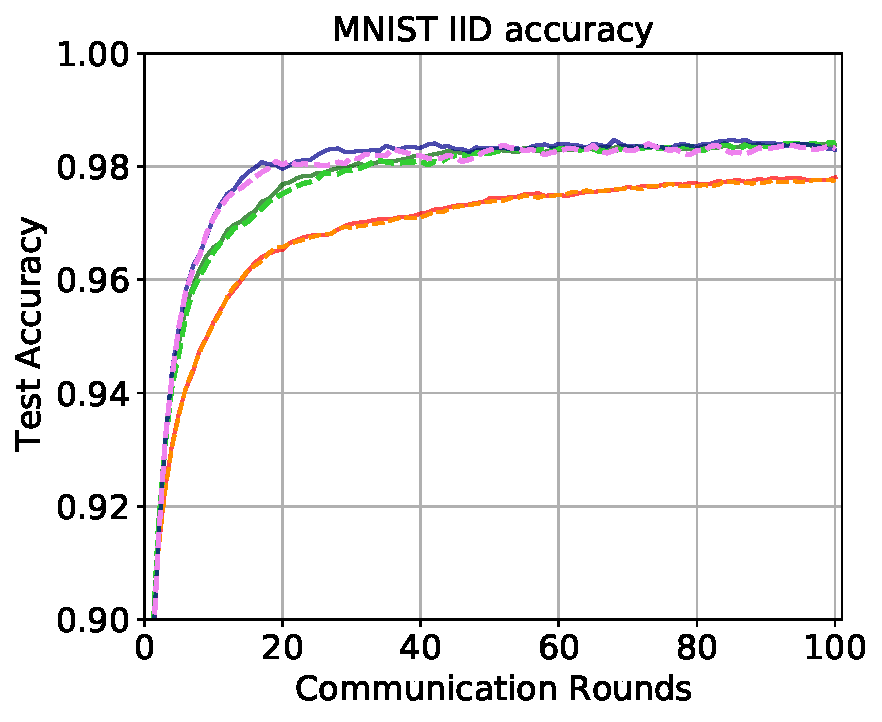
\includegraphics[width=.8\linewidth]{100perfig/mnist_iid.pdf}
  \label{fig:sub13}
\end{subfigure}
\begin{subfigure}{.5\textwidth}
  \centering
  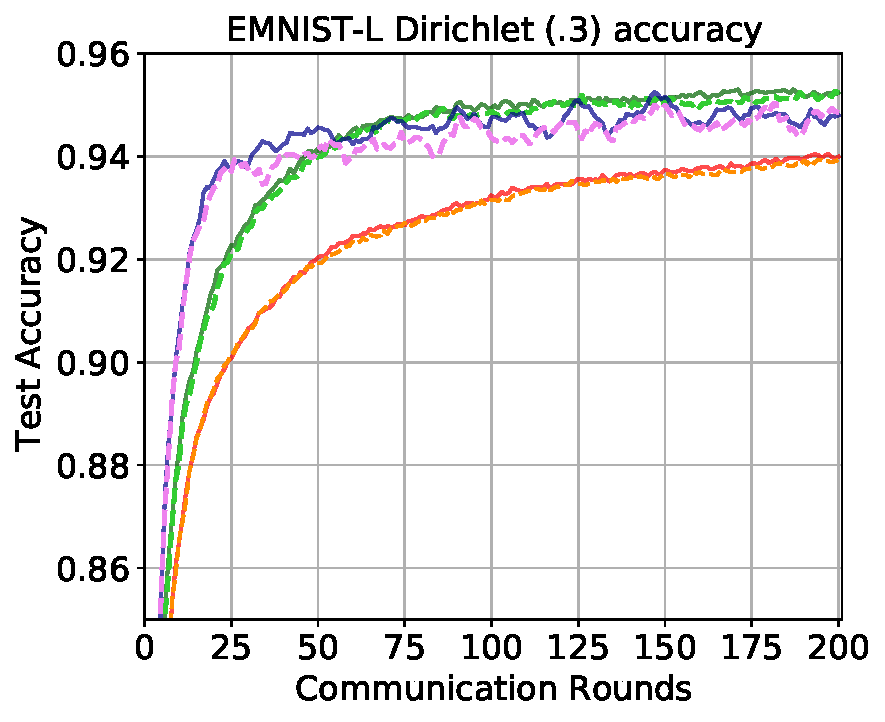
\includegraphics[width=.8\linewidth]{100perfig/emnist_0.3.pdf}
  \label{fig:sub14}
\end{subfigure}
\begin{subfigure}{.5\textwidth}
  \centering
  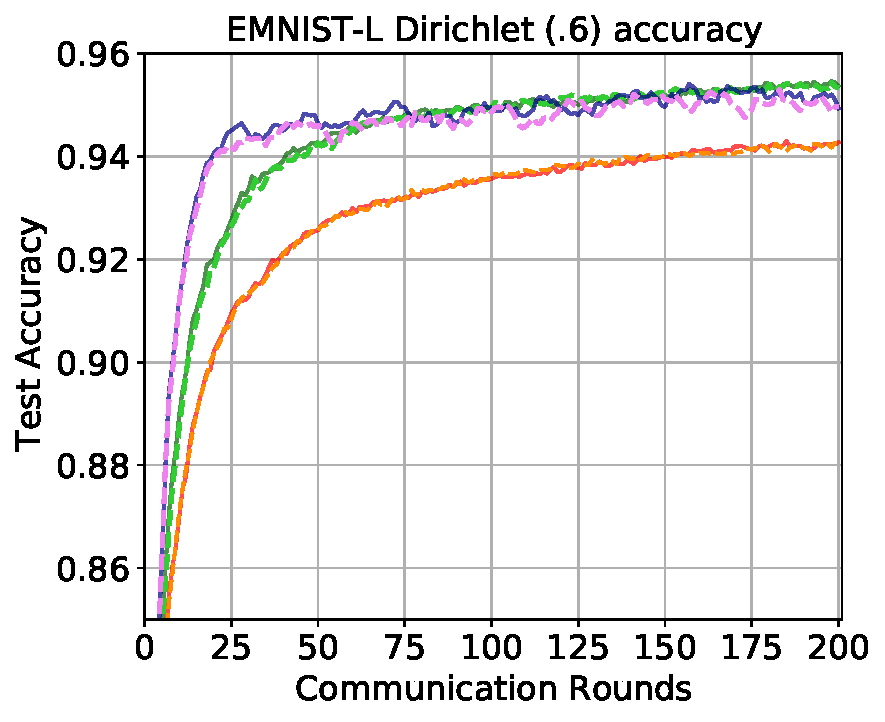
\includegraphics[width=.8\linewidth]{100perfig/emnist_0.6.pdf}
  \label{fig:sub15}
\end{subfigure}
\begin{subfigure}{.5\textwidth}
  \centering
  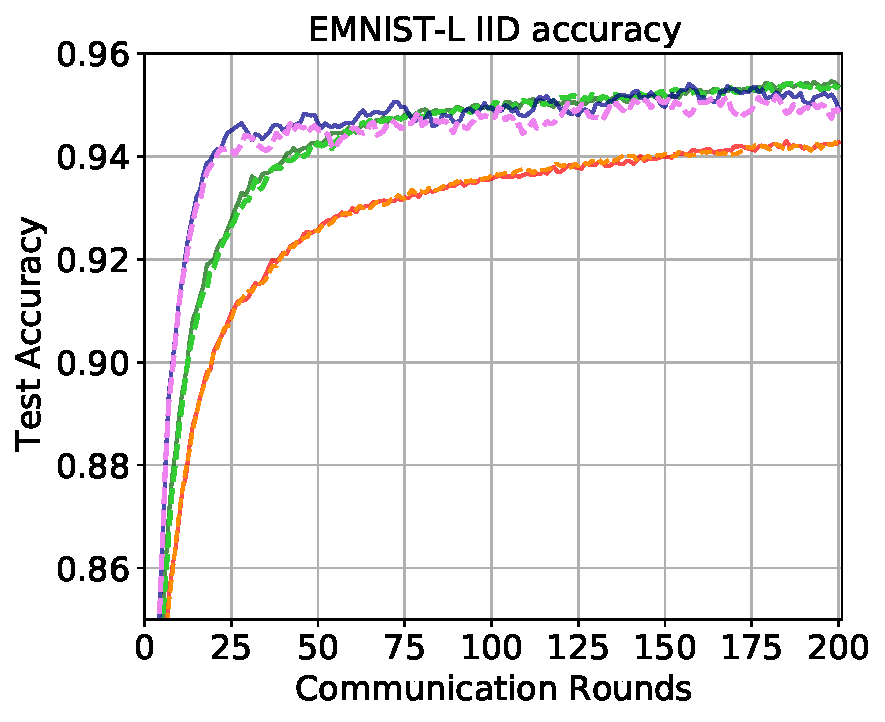
\includegraphics[width=.8\linewidth]{100perfig/emnist_iid.pdf}
  \label{fig:sub16}
\end{subfigure}
\begin{subfigure}{1\textwidth}
  \centering
  \includegraphics[width=1\linewidth]{textfigure/legend.pdf}
  \label{fig:sub17}
\end{subfigure}
\caption{Classification accuracy performance evaluated in MNIST, EMNIST-L datasets (100\% participation rate).}
\label{fig:100peracc1}
\end{figure}

\begin{figure}[ht!]
\begin{subfigure}{.5\textwidth}
  \centering
  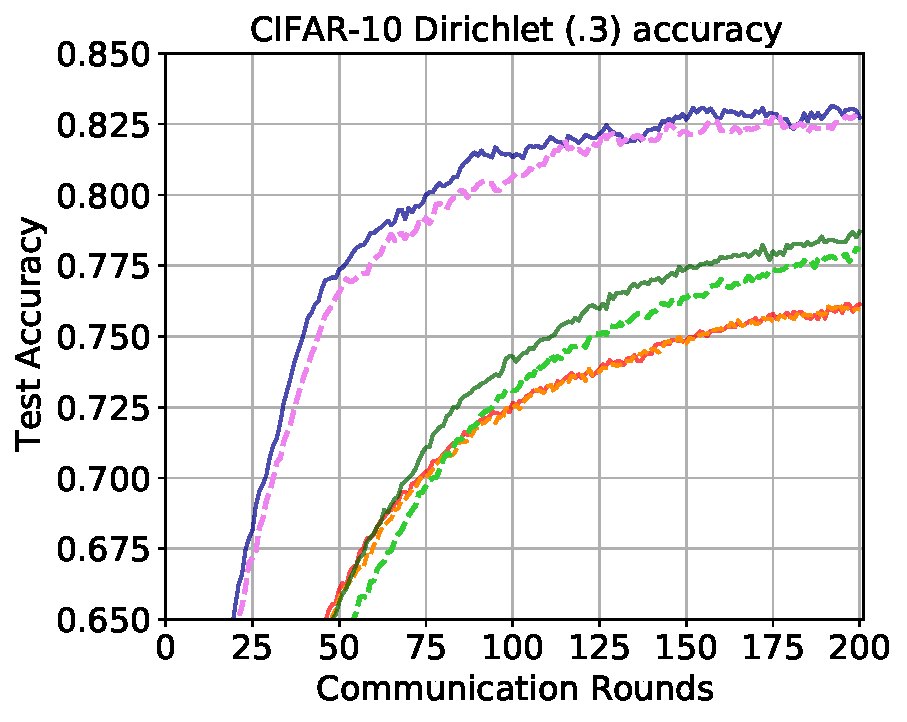
\includegraphics[width=.8\linewidth]{100perfig/cifar10_0.3.pdf}
  \label{fig:sub21}
\end{subfigure}
\begin{subfigure}{.5\textwidth}
  \centering
  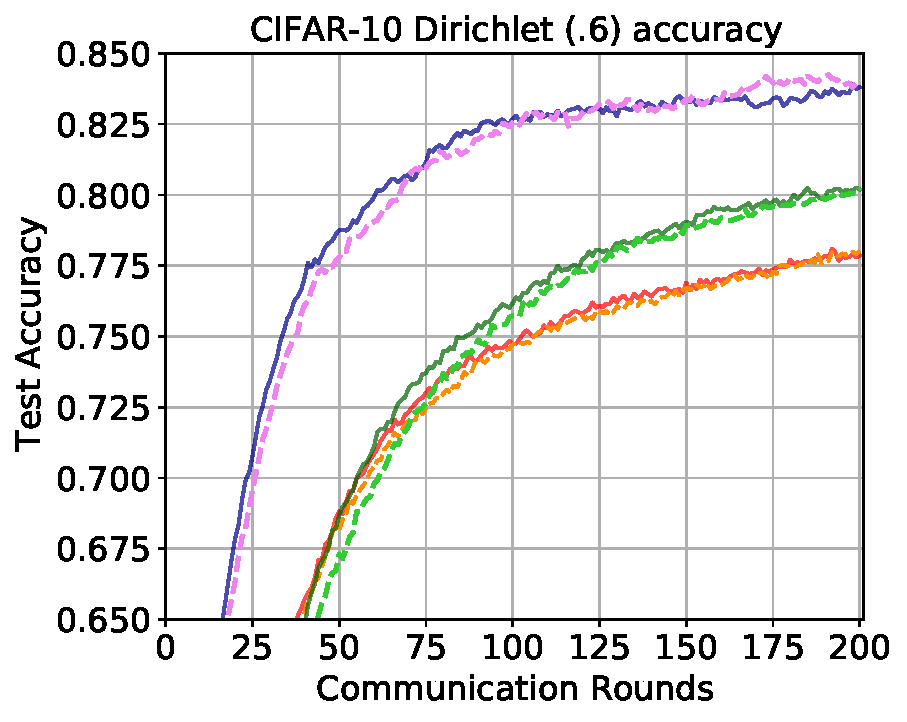
\includegraphics[width=.8\linewidth]{100perfig/cifar10_0.6.pdf}
  \label{fig:sub22}
\end{subfigure}
\begin{subfigure}{.5\textwidth}
  \centering
  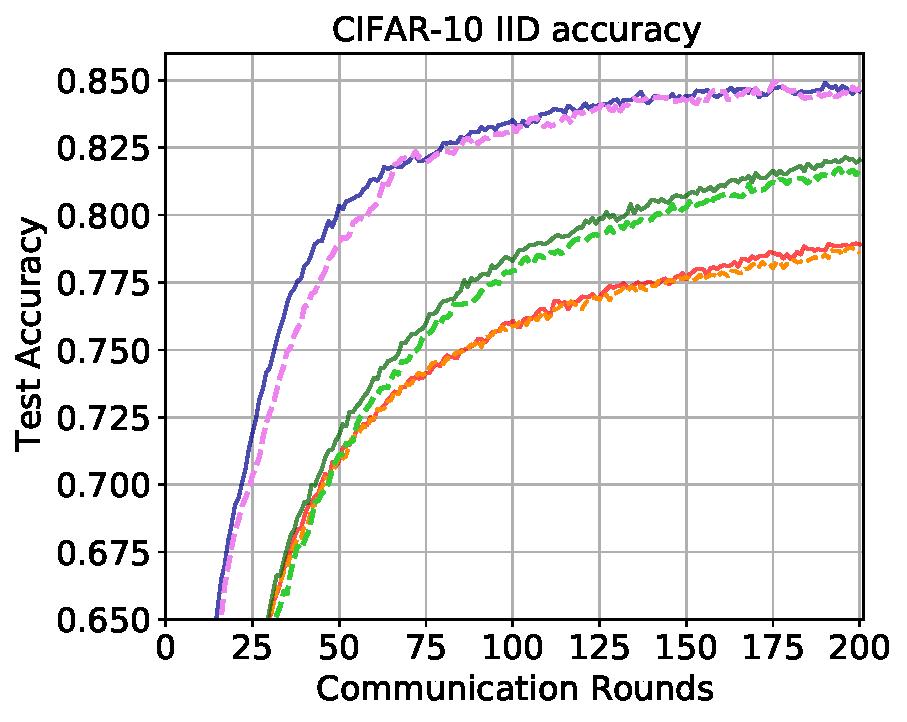
\includegraphics[width=.8\linewidth]{100perfig/cifar10_iid.pdf}
  \label{fig:sub23}
\end{subfigure}
\begin{subfigure}{.5\textwidth}
  \centering
  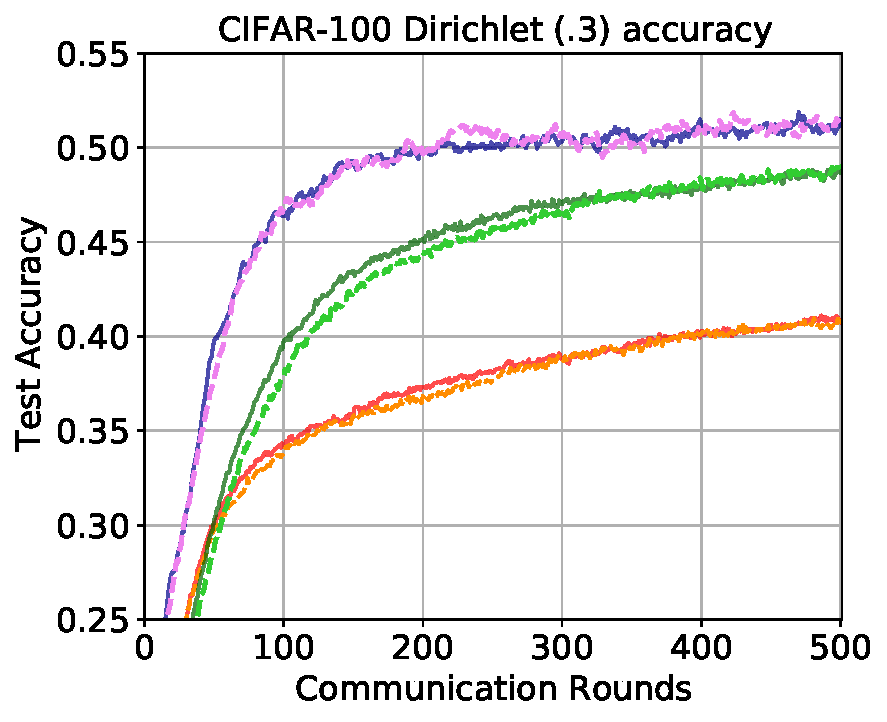
\includegraphics[width=.8\linewidth]{100perfig/cifar100_0.3.pdf}
  \label{fig:sub24}
\end{subfigure}
\begin{subfigure}{.5\textwidth}
  \centering
  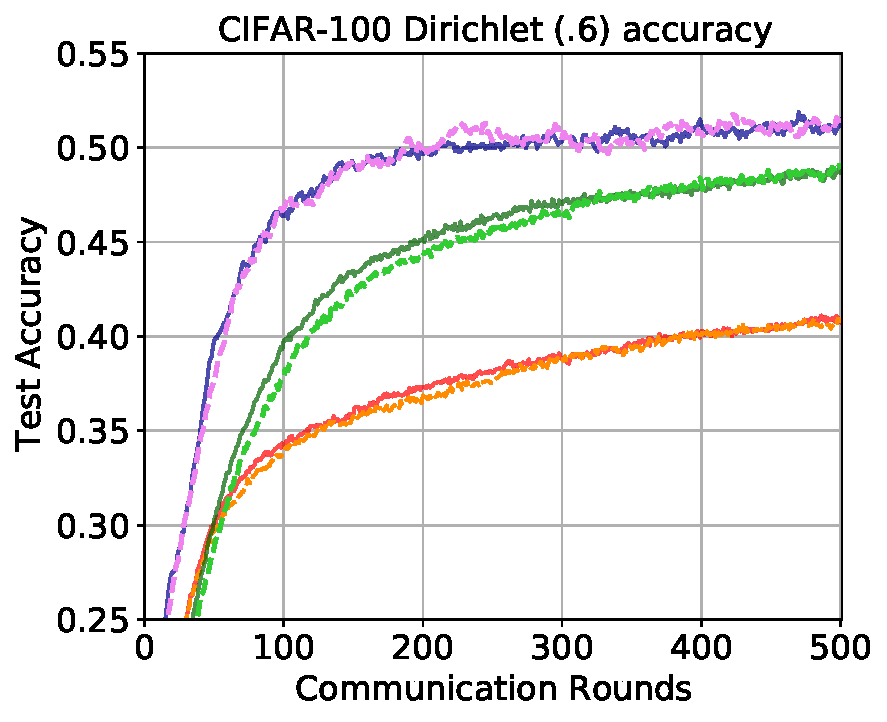
\includegraphics[width=.8\linewidth]{100perfig/cifar100_0.6.pdf}
  \label{fig:sub25}
\end{subfigure}
\begin{subfigure}{.5\textwidth}
  \centering
  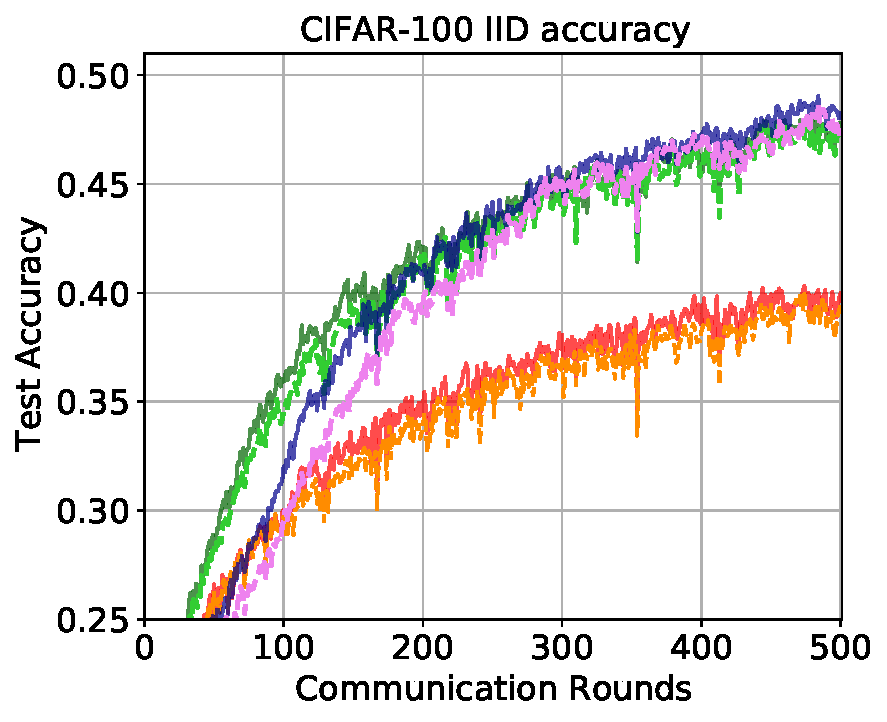
\includegraphics[width=.8\linewidth]{100perfig/cifar100_iid.pdf}
  \label{fig:sub26}
\end{subfigure}
\begin{subfigure}{1\textwidth}
  \centering
  \includegraphics[width=1\linewidth]{textfigure/legend.pdf}
  \label{fig:sub27}
\end{subfigure}
\caption{Classification accuracy performance evaluated in CIFAR-10 and CIFAR-100 datasets (100\% participation rate).}
\label{fig:100peracc2}
\end{figure}


\clearpage
\section{Proof}
%기존의 FedDyn과는 다른 부분만 남기고 제거
We utilize some techniques in FedDyn~\citep{Acar2021federated}. 
\subsection{Definition} \label{append_def}
We introduce a formal definition and properties that we will use.
\begin{definition}
A function $L_k$ is $\beta$-smooth if it satisfies
\begin{equation}\label{smooth1}
    \lVert \nabla L_k(x)- \nabla L_k(y) \rVert \le \beta \lVert x - y \rVert \ \  ~~~  \forall x,y.
\end{equation}
\end{definition}
If function $L_k$ is convex and $\beta$-smooth, it satisfies
\begin{equation}\label{smooth2}
   -\langle\nabla L_k(x), z-y\rangle\le -L_k(z) + L_k(y) + \frac{\beta}{2} \lVert z-x \rVert ^2 \ \    \forall x,y,z.
\end{equation}


As a consequence of the convexity and smoothness, the following property holds \citep[Theorem 2.1.5]{Nesterove2018}:
\begin{equation}\label{convex1}
    \frac{1}{2\beta m} \sum_{k\in [m]} \lVert \nabla L_k(x)-\nabla L_k(x_*) \rVert^2 \le \mathcal{R}(x)-\mathcal{R}(x_*) \ \   \forall x
\end{equation}
where $\mathcal{R}(x)=\frac{1}{m}\sum_{k=1}^m L_k(x)$ and $\nabla \mathcal{R}(x_*)=0$.

We will also use the relaxed triangle inequality \citep[Lemma 3]{Karimireddy2020scaffold}:
\begin{equation}\label{triangle}
    \left \lVert\sum_{j=1}^n v_j \right\rVert^2 \le n\sum_{j=1}^n \lVert v_j \rVert^2.
\end{equation}
%Third, norm inequality.
%\begin{equation}
%    \lVert a \rVert_1 \le \sqrt{n}\lVert %a\rVert _2
%\end{equation}
%, where $a$ is any vector and $n$, is a number of elements of the vector
\subsection{Proof of Theorem 3.1} \label{append_theorem}
%Some equations in Algorithm~\ref{algo:feddyn}
% \begin{align}
%     & \label{thetakt}\cdot\theta_{k}^{t} = \arg\underset{\theta}\min \: L_{k}\left ( \theta \right ) - \left< \nabla L_{k} (\theta_k^{t-1}), \theta\right> + \frac{\lambda_2}{2} \left\| \theta - \theta^{t-1}\right\|^{2}_{2}+ \lambda_1\left\|\theta - \theta^{t-1} \right\|_{1} \ \ \forall k \in [\mathcal{P}_t]\\
%     &\label{greadientLk}\cdot\nabla L_{k}\left ( \theta_{k}^{t} \right ) = \nabla L_{k}\left ( \theta_{k}^{t-1} \right ) - \lambda_2\left (\theta_{k}^{t} - \theta^{t-1} \right ) - \lambda_1  \cdot  \text{sign} \left (\theta_{k}^{t} - \theta^{t-1}  \right )\\
%     &\label{ht}\cdot h^{t} = h^{t-1} - \frac{\lambda_2}{m} \sum_{k\in \mathcal{P}_{t}}\left (\theta_{k}^{t} - \theta^{t-1} \right ) - \frac{\lambda_1}{m} \sum_{k \in \mathcal{P}_t}{\text{sign}(\theta_{k}^{t}-\theta^{t-1})}\\
%     &\label{thetat}\cdot \theta^{t} = \left ( \frac{1}{\left| \mathcal{P}_{t}\right|}\sum_{k \in \mathcal{P}_{t}} \theta_{k}^{t}\right ) - \frac{1}{\lambda_2}h^{t}
% \end{align}

The theorem that we will prove is as follows.
\begin{theorem}[Full statement of Theorem 3.1]\label{convergence_theorem}
Assume that the clients are uniformly randomly selected at each round and the individual loss functions $\{L_k\}_{k=1}^m$ are convex and $\beta$-smooth. Also assume that $\lambda_2>27\beta$. Then Algorithm~\ref{algo:feddyn} satisfies the following inequality: Letting $\mathcal{R}(\theta) = \frac{1}{m} \sum_{k \in [m]} L_k(\theta)$ and $    \theta_* =\underset{\theta}{\arg\min}\mathcal{R}(\theta)$,
\begin{align}
    \mathbb{E}\left[ \mathcal{R}\left( \frac{1}{T}\sum_{t=0}^{T-1}\gamma^t \right)-\mathcal{R}(\theta_*) \right]&\nonumber\le \frac{1}{T}\frac{1}{\kappa_0}(\mathbb{E}\lVert  \gamma^{0}-\theta_* \rVert^2+\kappa C_{0})+\frac{\kappa'}{\kappa_0} \cdot \lambda_1^2d\\
    &-\frac{1}{T}\frac{2\lambda_1}{\lambda_2 }\sum_{t=1}^T \left\langle({\gamma^{t-1}-\theta_*}),\frac{1}{m}\sum_{k\in [m]}\mathbb{E}[\mathrm{sign}(\tilde{\theta}_k^t-\theta^{t-1})]\right\rangle,
    %\sqrt{\frac{m}{P}}(\beta \lVert \theta^0-\theta_* \rVert+\frac{1}{\beta}\frac{1}{m}\sum_{k\in [m]}\lVert \nabla L_k (\theta_*) \rVert^2 ))
\end{align}

where
\begin{align*}
    \gamma^t &=\frac{1}{P}\sum_{k\in \mathcal{P}_t}\theta_k^t=\theta^t+\frac{1}{\lambda_2}h^t ~~~ \textrm{with } P = |\mathcal{P}_t|, \\
    \kappa &= \frac{10m}{P}\frac{1}{\lambda_2}\frac{\lambda_2+\beta}{\lambda_2^2-25\beta^2}, \\
    \kappa_0 &= \frac{2}{\lambda_2}\frac{\lambda_2^2-25\lambda_2\beta-50\beta^2}{\lambda_2^2-25\beta^2}, \\
    \kappa' &= \frac{5}{\lambda_2}\frac{\lambda_2+\beta}{\lambda_2^2-25\beta^2} = \kappa \cdot \frac{P}{2m}, \\
    C_0 &= \frac{1}{m}\sum_{k\in[m]}\mathbb{E}\lVert\nabla L_k(\theta_k^0)-\nabla L_k(\theta_*)\rVert, \\
    d &= \textrm{dim}(\theta).
\end{align*}
% $\mathcal{R}(\theta) = \frac{1}{m} \sum_{k \in [m]} L_k(\theta)$, 
% $\gamma^t=\frac{1}{P}\sum_{k\in \mathcal{P}_t}\theta_k^t=\theta^t+\frac{1}{\lambda_2}h^t$,and $\theta_*=\underset{\theta}{\arg\min}\mathcal{R}(\theta)$ and $d=\dim(\theta)$, $\kappa=\frac{10m}{P}\frac{1}{\lambda_2}\frac{\lambda_2+\beta}{\lambda_2^2-25\beta^2}, \kappa_0=\frac{2}{\lambda_2}\frac{\lambda_2^2-25\lambda_2\beta-50\beta^2}{\lambda_2^2-25\beta^2}$, $\kappa' = \frac{1}{5\lambda_2}\frac{\lambda_2+\beta}{\lambda_2^2-25\beta^2} = \kappa \cdot \frac{P}{2m}$, and $C_0=\frac{1}{m}\sum_{k\in[m]}\mathbb{E}\lVert\nabla L_k(\theta_k^0)-\nabla L_k(\theta_*)\rVert$.
\end{theorem}



To prove the theorem, define variables that will be used throughout the proof.
\begin{align}\label{tildetheta}
    \Tilde{\theta}_k^t &= \arg\underset{\theta}\min \: L_{k}\left ( \theta \right ) - \left< \nabla L_{k} (\theta_k^{t-1}), \theta\right> + \frac{\lambda_2}{2} \left\| \theta - \theta^{t-1}\right\|^{2}_{2}+ \lambda_1\left\|\theta - \theta^{t-1} \right\|_{1}\ \ \forall k \in [m] \\
\label{controlepsilon}
    C_t&=\frac{1}{m}\sum_{k\in [m]}\mathbb{E}\lVert \nabla L_k(\theta_k^t)-\nabla L_k(\theta_*) \rVert^2, \\
    \epsilon_t&=\frac{1}{m}\sum_{k\in[m]}\mathbb{E}\lVert \Tilde{\theta_k^t}-\gamma^{t-1} \rVert^2.
\end{align}
Note that $\Tilde{\theta}_k^t$ optimizes the $k$th loss function by assuming that the $k$th client ($k\in [m]$) is selected at round $t$. It is obvious that $\Tilde{\theta}_k^t = \theta_k^t$ if $k\in \mathcal{P}_t$. 
$C_t$ refers to the average of the expected differences between gradients of each individual model and the globally optimal model. Lastly, $\epsilon_t$ refers to the deviation of each client model from the average of local models. Remark that $C_t$ and $\epsilon_t$ approach zero if all clients' models converge to the globally optimal model, i.e., $\theta_k^t\rightarrow \theta_*$.
%\begin{theorem}
%The penalty norm such as $\ell_1$, $\ell_2$ norm does not asymptotically convergence rate. 
%\end{theorem}
%\begin{proof}

%x\end{proof}
















The following lemma expresses $h^t$, how much the averaged active devices' model deviates from the global model.
\begin{lemma}\label{linear h}
Algorithm \ref{algo:feddyn} satisfies 
\begin{equation}\label{htlinear}
    h^t= \frac{1}{m}\sum_{k\in [m]}\nabla L_k(\theta_k^t) 
\end{equation}
\end{lemma}
\begin{proof}
Starting from the update of $h^t$ in Algorithm \ref{algo:feddyn},
\begin{align*}
    h^t &= h^{t-1} - \frac{\lambda_2}{m}\sum_{k\in [m]}(\theta_k^t-\theta^{t-1})-\frac{\lambda_1}{m}\sum_{k\in [m]} \mathrm{sign}(\theta_k^t-\theta^{t-1})\\
    &= h^{t-1} - \frac{1}{m}\sum_{k\in [m]}(\nabla L_k(\theta_k^{t-1})-\nabla L_k(\theta_k^t)-\lambda_1\mathrm{sign}(\theta_k^t-\theta^{t-1})) -\frac{\lambda_1}{m}\sum_{k\in [m]}\mathrm{sign}(\theta_k^t-\theta^{t-1}) \\
    &=h^{t-1}-\frac{1}{m}\sum_{k\in [m]}(\nabla L_k (\theta_k^{t-1})-\nabla L_k(\theta_k^{t})),
\end{align*}
where the second equality follows from (\ref{eq:feddyn_first_l1}). By summing $h^t$ recursively, we have
\begin{equation*}
    h^t = h^0 + \frac{1}{m}\sum_{k\in [m]}\nabla L_k(\theta_k^t) - \frac{1}{m}\sum_{k\in [m]}\nabla L_k(\theta_k^0) = \frac{1}{m}\sum_{k\in [m]}\nabla L_k(\theta_k^t).
\end{equation*}
\end{proof}

The next lemma provides how much the average of local models changes by using only $t$ round parameters.
\begin{lemma}\label{differencegamma}
Algorithm~\ref{algo:feddyn} satisfies 
\begin{equation*}
    \mathbb{E}[\gamma^t-\gamma^{t-1}] = \frac{1}{\lambda_2 m}\sum_{k\in [m]}\mathbb{E}[-\nabla L_k(\Tilde{\theta_k^t})] -\frac{\lambda_1}{\lambda_2 m}\sum_{k\in [m]}\mathbb{E}[\mathrm{sign}(\Tilde{\theta_k^t}-\theta^{t-1})].
\end{equation*}
\end{lemma}
\begin{proof}
Starting from the definition of $\gamma^t$,
\begin{align}
    \mathbb{E} \left[\gamma^t-\gamma^{t-1} \right] &= \mathbb{E}\left[ \left(\frac{1}{P}\sum_{k\in \mathcal{P}_t}\theta_k^t \right)-\theta^{t-1}-\frac{1}{\lambda_2}h^{t-1} \right] \nonumber \\
    &= \mathbb{E}\left[\frac{1}{P}\sum_{k\in \mathcal{P}_t}(\theta_k^t-\theta^{t-1})-\frac{1}{\lambda_2}h^{t-1} \right] \nonumber \\
    &\label{differencegamma3} = \mathbb{E}\left[\frac{1}{\lambda_2 P}\sum_{k\in \mathcal{P}_t}(\nabla L_k(\theta_k^{t-1})-\nabla L_k(\theta_k^t)-\lambda_1 \mathrm{sign}(\theta_k^t-\theta^{t-1}))-\frac{1}{\lambda_2}h^{t-1} \right] \\
    &\label{differencegamma4} = \mathbb{E}\left[\frac{1}{\lambda_2 P}\sum_{k\in \mathcal{P}_t}(\nabla L_k(\theta_k^{t-1})-\nabla L_k(\Tilde{\theta_k^t})-\lambda_1 \mathrm{sign}(\Tilde{\theta_k^t}-\theta^{t-1}))-\frac{1}{\lambda_2}h^{t-1}\right]\\
    &\label{differencegamma5} = \mathbb{E}\left[\frac{1}{\lambda_2 m}\sum_{k\in [m]}(\nabla L_k(\theta_k^{t-1})-\nabla L_k(\Tilde{\theta_k^t})-\lambda_1 \mathrm{sign}(\Tilde{\theta_k^t}-\theta^{t-1}))-\frac{1}{\lambda_2}h^{t-1} \right]\\
    &\label{differencegamma6} = \frac{1}{\lambda_2 m}\sum_{k\in [m]}\mathbb{E}[-\nabla L_k(\Tilde{\theta_k^t})]-\frac{\lambda_1}{\lambda_2 m}\sum_{k\in [m]}\mathbb{E}[\mathrm{sign}(\Tilde{\theta_k^t}-\theta^{t-1})],
    %&\label{differencegamma7}\approx \frac{1}{\lambda_2 m}\sum_{k\in [m]}\mathbb{E}[-\nabla L_k(\Tilde{\theta_k^t})],
\end{align}
%where (\ref{differencegamma1}) follows from definition of $\gamma_t$ and
where (\ref{differencegamma3}) follows from (\ref{eq:feddyn_first_l1}), (\ref{differencegamma4}) follows since $\tilde{\theta}_k^t=\theta_k^t$ if $k\in\mathcal{P}_t$, and (\ref{differencegamma5}) follows since clients are randomly chosen. The last equality is due to Lemma \ref{linear h}.
\end{proof}
%(\ref{differencegamma6}) follows from (\ref{htlinear}) and (\ref{differencegamma7}) follows from following Lemma.  (\ref{htlinear}) and (\ref{differencegamma7}) are consistent with the equation of FedDyn~\citep{Acar2021federated}.




%$\mu$ is equal to 0, $\mathbb{E}[\mathrm{sign}(\Tilde{\theta_k^t}-\theta^{t-1})]$ will be 0. 
%sign을 cumulative distribution function으로 바꾸었고, 이는 theta_k^t의 평균과 theta^t-1의 차이가 작을수록 mu가 0에 수렴하여 phi함수가 1/2이 되고 곧 0으로 수렴함. 그리고, mu가 0이 아니더라도 1에서 양수를 뺀 값이므로 굉장히 작은 수이고, lambda_1와 곱했으므로 무시할 수 있는 숫자가 됨.

Next, note that Algorithm~\ref{algo:feddyn} is the same as that of FedDyn except for the $\ell_1$-norm penalty. As this new penalty does not affect derivations of $C_t$, $\epsilon_t$, and $\mathbb{E}\lVert \gamma^t-\gamma^{t-1} \rVert^2$ in FedDyn~\citep{Acar2021federated}, we can obtain the following bounds on them. Proofs are omitted for brevity.% $\mathbb{E}\lVert \gamma^t-\theta_* \rVert^2$ terms can be found as in FedDyn~\citep{Acar2021federated}:
% we have to find bound of $C_t$, $\epsilon_t$ and $\mathbb{E}\lVert \gamma^t-\gamma^{t-1} \rVert^2$, $\mathbb{E}\lVert \gamma^t-\theta_* \rVert^2$ term. we use the following inequalities which are in line with FedDyn~\citep{Acar2021federated}:
\begin{align}
    &\mathbb{E}\lVert h^t \rVert^2 \le C_t\label{boundh}\\
    &C_t\label{boundC}\le \left(1-\frac{P}{m}\right) C_{t-1}+\frac{2\beta^2P}{m}\epsilon_t+\frac{4\beta P}{m}\mathbb{E}[\mathcal{R}(\gamma^{t-1})-\mathcal{R}(\theta_*)]\\
    &\mathbb{E}\lVert \gamma^t-\gamma^{t-1} \rVert^2 \label{MSEgamma}\le \frac{1}{m} \sum_{k\in [m]}\mathbb{E} [\lVert \Tilde{\theta_k^t}-\gamma^{t-1}\rVert ^2]=\epsilon_t
\end{align}
\begin{lemma}\label{msegammatheta}
Given model parameters at the round $(t-1)$, Algorithm ~\ref{algo:feddyn} satisfies
\begin{align}
    \mathbb{E}\lVert \gamma^t-\theta_* \rVert^2\le& 
    \mathbb{E}\lVert \gamma^{t-1}-\theta_* \rVert^2-\frac{2}{\lambda_2}\mathbb{E}[\mathcal{R}(\gamma^{t-1})-\mathcal{R}(\theta_*)]+\frac{\beta}{\lambda_2}\epsilon_t+\mathbb{E}\lVert \gamma^t-\gamma^{t-1} \rVert^2\\
    &-\frac{2\lambda_1}{\lambda_2 m}(\gamma^{t-1}-\theta_*)\sum_{k\in [m]}\mathbb{E}[\textrm{sign}(\tilde{\theta}_k^t-\theta^{t-1})],
\end{align}
where the expectations are taken assuming parameters at the round $(t-1)$ are given.
\end{lemma}
\begin{proof}
\begin{align}
    \mathbb{E}\lVert \gamma^t-\theta_* \rVert^2 
    &\nonumber=\mathbb{E}\lVert \gamma^{t-1}-\theta_*+\gamma^t-\gamma^{t-1} \rVert^2\\ 
    &\nonumber=\mathbb{E}\lVert \gamma^{t-1}-\theta_* \rVert^2+2\mathbb{E}[ \left\langle \gamma^{t-1}-\theta_*,\gamma^t-\gamma^{t-1} \right\rangle]+\mathbb{E}\lVert \gamma^t-\gamma^{t-1} \rVert^2\\
    &\nonumber\label{gammatheta1}=\mathbb{E}\lVert \gamma^{t-1}-\theta_* \rVert^2+\mathbb{E}\lVert \gamma^t-\gamma^{t-1} \rVert^2\\ 
    &+\frac{2}{\lambda_2 m}\sum_{k\in [m]}\mathbb{E}\left[ \left\langle \gamma^{t-1}-\theta_*,-\nabla L_k(\Tilde{\theta}_k^t)-\lambda_1(\mathrm{sign}(\tilde{\theta}_k^t-\theta^{t-1})) \right\rangle\right]
    \\
    &\le \label{gammatheta2} \nonumber\mathbb{E}\lVert \gamma^{t-1}-\theta_* \rVert^2+\mathbb{E}\lVert \gamma^t-\gamma^{t-1} \rVert^2\\ 
    &\nonumber+\frac{2}{\lambda_2 m}\sum_{k\in [m]}\mathbb{E}[L_k(\theta_*)-L_k(\gamma^{t-1})+\frac{\beta}{2}\lVert \Tilde{\theta}_k^t-\gamma^{t-1} \rVert^2]\\ 
    &+\frac{2}{\lambda_2 m}\sum_{k\in [m]}\mathbb{E}\left[ \left\langle \gamma^{t-1}-\theta_*,-\lambda_1\mathrm{sign}(\tilde{\theta}_k^t-\theta^{t-1}) \right\rangle\right]\\
    &= \label{gammatheta3}\nonumber\mathbb{E}\lVert \gamma^{t-1}-\theta_* \rVert^2+\mathbb{E}\lVert \gamma^t-\gamma^{t-1} \rVert^2-\frac{2}{\lambda_2}\mathbb{E}[\mathcal{R}(\gamma^{t-1})-\mathcal{R}(\theta_*)]+\frac{\beta}{\lambda_2}\epsilon_t\\ 
    &-\frac{2\lambda_1}{\lambda_2 m}\sum_{k\in [m]}\mathbb{E}\left[\left\langle \gamma^{t-1}-\theta_*,\mathrm{sign}(\tilde{\theta}_k^t-\theta^{t-1})\right\rangle \right]\\ 
    &\nonumber\label{gammatheta4}=\mathbb{E}\lVert \gamma^{t-1}-\theta_* \rVert^2+\mathbb{E}\lVert \gamma^t-\gamma^{t-1} \rVert^2-\frac{2}{\lambda_2}\mathbb{E}[\mathcal{R}(\gamma^{t-1})-\mathcal{R}(\theta_*)]+\frac{\beta}{\lambda_2}\epsilon_t\\
    &-\frac{2\lambda_1}{\lambda_2 }\left\langle {\gamma^{t-1}-\theta_*}, \frac{1}{m}\sum_{k\in [m]}\mathbb{E}[\mathrm{sign}(\tilde{\theta}_k^t-\theta^{t-1})]\right\rangle
    %&\label{gammatheta5}\le\mathbb{E}\lVert \gamma^{t-1}-\theta_* \rVert^2-\frac{2}{\lambda_2}\mathbb{E}[\mathcal{R}(\gamma^{t-1})-\mathcal{R}(\theta_*)]+\frac{\beta}{\lambda_2}\epsilon_t+\mathbb{E}\lVert \gamma^t-\gamma^{t-1} \rVert^2,
\end{align}
where (\ref{gammatheta1}) follows from Lemma~\ref{differencegamma}, (\ref{gammatheta2}) follows from (\ref{smooth2}), and (\ref{gammatheta3}) follows from the definitions of $\mathcal{R}(\cdot)$ and $\epsilon_t$.% (\ref{smooth2}), and (\ref{gammatheta3}) follows from (\ref{smooth1}). 
\end{proof}
\begin{lemma}\label{boundepsilon}
Algorithm \ref{algo:feddyn} satisfies 
\begin{equation*}
    (1-5\frac{\beta^2}{\lambda_2^2})\epsilon_t\le10\frac{1}{\lambda_2^2}C_{t-1}+10\beta\frac{1}{\lambda_2^2}\mathbb{E}[\mathcal{R}(\gamma^{t-1})-\mathcal{R}(\theta_*)]+\frac{5\lambda_1^2}{\lambda_2^2}d
\end{equation*}
\end{lemma}
\begin{proof}
Starting from the definitions of $\epsilon_t$ and $\gamma^t$,
\begin{align}
    \epsilon_t &=\frac{1}{m}\sum_{k\in[m]}\mathbb{E}\lVert \Tilde{\theta_k^t}-\gamma^{t-1} \rVert^2 \nonumber \\
    &= \frac{1}{m}\sum_{k\in[m]}\mathbb{E}\lVert \Tilde{\theta_k^t}-\theta^{t-1}-\frac{1}{\lambda_2}h^{t-1}\rVert^2 \nonumber \\
    &\label{epsilon3}= \frac{1}{\lambda_2^2}\frac{1}{m}\sum_{k\in [m]}\mathbb{E}\lVert \nabla L_k(\theta_k^{t-1}) -\nabla L_k(\Tilde{\theta}_k^t)-\lambda_1\mathrm{sign}(\theta_k^t-\theta^{t-1}) -h^{t-1} \rVert^2\\
    &= \frac{1}{\lambda_2^2}\frac{1}{m}\sum_{k\in [m]}\mathbb{E}\lVert \nabla L_k(\theta_k^{t-1}) -\nabla L_k(\theta_*) + \nabla L_k(\theta_*) -\nabla L_k(\gamma^{t-1}) \nonumber \\
    & +\nabla L_k(\gamma^{t-1}) -\nabla  L_k(\Tilde{\theta}_k^t) - \lambda_1\mathrm{sign}(\theta_k^t-\theta^{t-1}) -h^{t-1} \rVert^2 \nonumber \\
    &\le \nonumber\frac{5}{\lambda_2^2}\frac{1}{m}\sum_{k\in[m]}\mathbb{E}\lVert \nabla L_k(\theta_k^{t-1})-\nabla L_k(\theta_*) \rVert^2 
    + \frac{5}{\lambda_2^2}\frac{1}{m}\sum_{k\in[m]}\mathbb{E}\lVert \nabla L_k(\gamma_k^{t-1})-\nabla L_k(\theta_*) \rVert^2 \nonumber \\
    &\ \ \ \ \ + \frac{5}{\lambda_2^2}\frac{1}{m}\sum_{k\in[m]}\mathbb{E}\lVert \nabla L_k(\Tilde{\theta}_k^t)-\nabla L_k(\gamma^{t-1}) \rVert^2
    +\frac{5}{\lambda_2^2}\mathbb{E}\lVert \lambda_1\mathrm{sign}(\theta_k^t-\theta^{t-1}) \rVert^2+\frac{5}{\lambda_2^2}\mathbb{E}\lVert h^{t-1} \rVert^2 \label{epsilon5} \\
    &\label{epsilon6}\le \nonumber\frac{5}{\lambda_2^2}\frac{1}{m}\sum_{k\in[m]}\mathbb{E}\lVert \nabla L_k(\theta_k^{t-1})-\nabla L_k(\theta_*) \rVert^2 
    + \frac{5}{\lambda_2^2}\frac{1}{m}\sum_{k\in[m]}\mathbb{E}\lVert \nabla L_k(\gamma_k^{t-1})-\nabla L_k(\theta_*) \rVert^2 \\
    & + \frac{5}{\lambda_2^2}\frac{1}{m}\sum_{k\in[m]}\mathbb{E}\lVert \nabla L_k(\Tilde{\theta}_k^t)-\nabla L_k(\gamma^{t-1}) \rVert^2
    +\frac{5\lambda_1^2}{\lambda_2^2}d+\frac{5}{\lambda_2^2}C_{t-1}\\
    &\label{epsilon7}\le \frac{5}{\lambda_2^2}C_{t-1}
    + \frac{5}{\lambda_2^2}2\beta\ \mathbb{E}[\mathcal{R}(\gamma^{t-1})-\mathcal{R}(\theta_*)] 
    + \frac{5\beta^2}{\lambda_2^2}\frac{1}{m}\sum_{k\in[m]}\mathbb{E}\lVert \Tilde{\theta}_k^t -\gamma^{t-1}\rVert^2
    +\frac{5\lambda_1^2}{\lambda_2^2}d+\frac{5}{\lambda_2^2}C_{t-1}\\
    &= \frac{10}{\lambda_2^2}C_{t-1}+\frac{10\beta}{\lambda_2^2}\mathbb{E}[\mathcal{R}(\gamma^{t-1})-\mathcal{R}(\theta_*)]+\frac{5\beta^2}{\lambda_2^2}\epsilon_t+\frac{5\lambda_1^2}{\lambda_2^2}d, \nonumber
\end{align}
where (\ref{epsilon3}) follows from (\ref{eq:feddyn_first_l1}), (\ref{epsilon5}) follows from the relaxed triangle inequality (\ref{triangle}), (\ref{epsilon6}) follows from (\ref{boundh}), and (\ref{epsilon7}) follows from the definition of $C_t$, the smoothness, and (\ref{convex1}). The last equality follows from the definition of $\epsilon_t$.  
% where $d$ is dimension of $\theta_k^t$. (\ref{epsilon2}) follows from definition of $\gamma^t$ and (\ref{epsilon3}) follows from (\ref{eq:feddyn_first_l1_noise}) and (\ref{epsilon5}) follows from relaxed triangle inequality(\ref{triangle}) and
% (\ref{epsilon6}) follows from (\ref{boundh}) and (\ref{epsilon7}) follows from (\ref{smooth1}) and (\ref{convex1}) and (\ref{epsilon8}) follows from (\ref{MSEgamma}). 
\end{proof}

After multiplying (\ref{boundC}) by $\kappa(=10\frac{m}{P}\frac{1}{\lambda_2}\frac{\lambda_2+\beta}{\lambda_2^2-25\beta^2})$, we obtain the following theorem by summing (\ref{msegammatheta}) and scaled version of (\ref{MSEgamma}).


%\begin{align}
%    &\kappa C_t\le \kappa(1-\frac{P}{m})C_{t-1}+\kappa\frac{2\beta^2P}{m}\epsilon_t+\kappa\frac{4\beta P}{m}\mathbb{E}[\mathcal{R}(\gamma^{t-1})-\mathcal{R}(\theta_*)]\\
%    &\mathbb{E}\lVert \gamma^t-\theta_* \rVert^2\le 
%    \mathbb{E}\lVert \gamma^{t-1}-\theta_*\rVert^2-\frac{2}{\lambda_2}\mathbb{E}[\mathcal{R}(\gamma^{t-1})-\mathcal{R}(\theta_*)]+\frac{\beta}{\lambda_2}\epsilon_t+\mathbb{E}\lVert \gamma^t-\gamma^{t-1} \rVert^2
%\end{align}

















\begin{theorem}\label{convergence_lemma}
Given model parameters at the round $(t-1)$, Algorithm~\ref{algo:feddyn} satisfies 
\begin{align*}
    \kappa_0\mathbb{E}[\mathcal{R}(\gamma^{t-1})-\mathcal{R}(\theta_*)]&\le (\mathbb{E}\lVert  \gamma^{t-1}-\theta_* \rVert^2+\kappa C_{t-1})-(\mathbb{E}\lVert \gamma^t -\theta_*\rVert^2+\kappa C_t)+\kappa\frac{P}{2m}\lambda_1^2\\
    &-\frac{2\lambda_1}{\lambda_2 }\left\langle \gamma^{t-1}-\theta_*,\frac{1}{m}\sum_{k\in [m]}\mathbb{E}[\mathrm{sign}(\tilde{\theta}_k^t-\theta^{t-1})]\right\rangle.
\end{align*}
% \begin{align*}
%     \mathbb{E}\lVert \gamma^t -\theta_*\rVert^2+\kappa C_t
%     &\le \mathbb{E}\lVert  \gamma^{t-1}-\theta_* \rVert^2+\kappa C_{t-1}-\kappa_0\mathbb{E}[\mathcal{R}(\gamma^{t-1})-\mathcal{R}(\theta_*)] \\
%     &~~~~~~~~~~~~~~~ +\kappa\frac{P}{2m}\lambda_1^2 d -\frac{2\lambda_1}{\lambda_2 m}({\gamma^{t-1}-\theta_*})\sum_{k\in [m]}\mathbb{E}[\mathrm{sign}(\tilde{\theta}_k^t-\theta^{t-1})],
% \end{align*}
where $\kappa=10\frac{m}{P}\frac{1}{\lambda_2}\frac{\lambda_2+\beta}{\lambda_2^2-25\beta^2},\kappa_0=\frac{2}{\lambda_2}\frac{\lambda_2^2-25\lambda_2\beta-50\beta^2}{\lambda_2^2-25\beta^2}$. Note that the expectations taken above are conditional expectations given model parameters at time $(t-1)$.
\end{theorem}
\begin{proof}
Summing Lemma~$\ref{msegammatheta}$ and $\kappa$-scaled version of (\ref{boundC}), we have
\begin{align}
    &\mathbb{E}\lVert \gamma^t-\theta_* \rVert^2+\kappa C_t \nonumber \\
    &\le\nonumber \mathbb{E}\lVert \gamma^{t-1}-\theta_*\rVert^2 + \kappa C_{t-1}  -\kappa\frac{P}{m}C_{t-1}+\kappa\frac{2\beta^2P}{m}\epsilon_t+\kappa\frac{4\beta P}{m}\mathbb{E}[\mathcal{R}(\gamma^{t-1})-\mathcal{R}(\theta_*)] \\
    &~ - \frac{2}{\lambda_2}\mathbb{E}[\mathcal{R}(\gamma^{t-1})-\mathcal{R}(\theta_*)]+\frac{\beta}{\lambda_2}\epsilon_t+\mathbb{E}\lVert \gamma^t-\gamma^{t-1} \rVert^2 -\frac{2\lambda_1}{\lambda_2 m}({\gamma^{t-1}-\theta_*})\sum_{k\in [m]}\mathbb{E}[\mathrm{sign}(\tilde{\theta}_k^t-\theta^{t-1})]. \label{confuse} 
\end{align}
As $\mathbb{E}\lVert \gamma^t-\gamma^{t-1} \rVert^2 \le \epsilon_t$ by ($\ref{MSEgamma}$), we have
%We telescope $\epsilon_t$ term and  $\mathbb{E}\lVert \gamma^t-\gamma^{t-1} \rVert^2$ term of (\ref{confuse}).
\begin{align}\label{confuseepsilon}
    \kappa\frac{2\beta^2P}{m}\epsilon_t+\frac{\beta}{\lambda_2}\epsilon_t+\mathbb{E}\lVert \gamma^t-\gamma^{t-1} \rVert^2
    &\le \kappa\frac{2\beta^2P}{m}\epsilon_t+\frac{\beta}{\lambda_2}\epsilon_t+\epsilon_t.
\end{align}
This can be further bounded as follows.%Then we rewrite (\ref{confuseepsilon}) by using Theorem~\ref{boundepsilon}.
\begin{align*}
    (\ref{confuseepsilon})
    &= \left( 10\frac{m}{P}\frac{1}{\lambda_2}\frac{\lambda_2+\beta}{\lambda_2^2-25\beta^2}\cdot\frac{2\beta^2P}{m} + \frac{\beta}{\lambda_2}+1  \right) \epsilon_t\\
    &=\frac{1}{\lambda_2 (\lambda_2^2-25\beta^2)} \left( 20(\lambda_2+\beta)\beta^2+\beta(\lambda_2^2-25\beta^2)+\lambda_2(\lambda_2^2-25\beta^2) \right) \epsilon_t\\
    &=\frac{\lambda_2(\lambda_2+\beta)}{\lambda_2^2-25\beta^2} \left(1-5\frac{\beta^2}{\lambda_2^2}\right) \epsilon_t\\
    &\le \frac{\lambda_2(\lambda_2+\beta)}{\lambda_2^2-25\beta^2} \left( \frac{10}{\lambda_2^2}C_{t-1} + \frac{10\beta}{\lambda_2^2}\mathbb{E}[\mathcal{R}(\gamma^{t-1})-\mathcal{R}(\theta_*)]+\frac{5\lambda_1^2}{\lambda_2^2}d \right) \\
    &=\kappa\frac{P}{m} C_{t-1}+\kappa\frac{\beta P}{m}\mathbb{E}[\mathcal{R}(\gamma^{t-1})-\mathcal{R}(\theta_*)]+\kappa\frac{P}{2m}\lambda_1^2d,
\end{align*}
where the inequality follows from Lemma~\ref{boundepsilon}. Then, (\ref{confuse}) term will be 
\begin{align*}
    \mathbb{E}\lVert \gamma^t-\theta_* \rVert^2+\kappa C_t &\le 
    %\mathbb{E}\lVert \gamma^{t-1}-\theta_*\rVert^2 + \kappa C_{t-1}+\{\frac{5\kappa\beta P}{m}-\frac{2}{\lambda_2}\}\mathbb{E}[\mathcal{R}(\gamma^{t-1})-\mathcal{R}(\theta_*)]+\frac{2\lambda_1}{\lambda_2}+\kappa\frac{P}{2m}\lambda_1^2d\\
    \mathbb{E}\lVert \gamma^{t-1}-\theta_*\rVert^2 + \kappa C_{t-1}-\kappa_0\mathbb{E}[\mathcal{R}(\gamma^{t-1})-\mathcal{R}(\theta_*)]+\kappa\frac{P}{2m}\lambda_1^2d\\
    &-\frac{2\lambda_1}{\lambda_2 }\left\langle {\gamma^{t-1}-\theta_*}, \frac{1}{m}\sum_{k\in [m]}\mathbb{E}[\mathrm{sign}(\tilde{\theta}_k^t-\theta^{t-1})]\right\rangle.
\end{align*}
Rearranging terms, we prove the claim.
\end{proof}








% Then, we can rewrite \ref{convergence_lemma} as the following way,
% \begin{align}\label{kappa0R}
%     \nonumber\kappa_0\mathbb{E}[\mathcal{R}(\gamma^{t-1})-\mathcal{R}(\theta_*)]&\le (\mathbb{E}\lVert  \gamma^{t-1}-\theta_* \rVert^2+\kappa C_{t-1})-(\mathbb{E}\lVert \gamma^t -\theta_*\rVert^2+\kappa C_t)+\kappa\frac{P}{2m}\lambda_1^2\\
%     &~~~~-\frac{2\lambda_1}{\lambda_2 m}({\gamma^{t-1}-\theta_*})\sum_{k\in [m]}\mathbb{E}[\mathrm{sign}(\tilde{\theta}_k^t-\theta^{t-1})].
% \end{align}
 
 Now we are ready to prove the main claim by combining all lemmas. Let us take the sum on both sides of Lemma~\ref{convergence_lemma} over $t=1, \ldots, T$. Then, telescoping gives us
 %Then, we get the following inequality by summing recursively:
\begin{align*}
    \kappa_0\sum_{t=1}^T\mathbb{E}[\mathcal{R}(\gamma^{t-1})-\mathcal{R}(\theta_*)]&\le (\mathbb{E}\lVert  \gamma^{0}-\theta_* \rVert^2+\kappa C_{0})-(\mathbb{E}\lVert \gamma^T -\theta_*\rVert^2+\kappa C_T)+T(\kappa\frac{P}{2m}\lambda_1^2)\\
    &-\frac{2\lambda_1}{\lambda_2 }\sum_{t=1}^T \left \langle \gamma^{t-1}-\theta_*,\frac{1}{m}\sum_{k\in [m]}\mathbb{E}[\mathrm{sign}(\tilde{\theta}_k^t-\theta^{t-1})] \right\rangle.
\end{align*}
Since $\kappa$ is positive if $\lambda_2>27\beta$, we can eliminate the negative term in the middle. Then,
\begin{align*}
    \kappa_0\sum_{t=1}^T\mathbb{E}[\mathcal{R}(\gamma^{t-1})-\mathcal{R}(\theta_*)]&\le \mathbb{E}\lVert  \gamma^{0}-\theta_* \rVert^2+\kappa C_{0}+T(\kappa\frac{P}{2m}\lambda_1^2d)\\
    &-\frac{2\lambda_1}{\lambda_2 } \sum_{t=1}^T\left\langle \gamma^{t-1}-\theta_*, \frac{1}{m}\sum_{k\in [m]} \mathbb{E}[\mathrm{sign}(\tilde{\theta}_k^t-\theta^{t-1})]\right\rangle.
\end{align*}
Dividing by $T$ and applying Jensen's inequality,
\begin{align}\label{summingresult}
    \mathbb{E} \left[ \mathcal{R}(\frac{1}{T}\sum_{t=0}^{T-1}\gamma^t)-\mathcal{R}(\theta_*) \right] &\le\frac{1}{T}\frac{1}{\kappa_0}(\mathbb{E}\lVert  \gamma^{0}-\theta_* \rVert^2+\kappa C_{0})+\frac{1}{\kappa_0}(\kappa\frac{P}{2m}\lambda_1^2d)\nonumber\\
    &-\frac{1}{T}\frac{2\lambda_1}{\lambda_2 }\sum_{t=1}^T\left\langle \gamma^{t-1}-\theta_*, \frac{1}{m}\sum_{k\in [m]}\mathbb{E}[\mathrm{sign}(\tilde{\theta}_k^t-\theta^{t-1})]\right\rangle,
\end{align}
which completes the proof of Theorem~\ref{convergence_theorem}.























%this should go to the end of the proof to argue this additional term is negligible
\subsection{Discussion on Convergence}\label{sec:disscusion}

% The following discussion and lemma provide that the second and the third term of (\ref{feddynconvergence}) is a negligible effect.
% \begin{lemma}Let $x={\theta}_k^t-\theta^{t-1}$ and $\mu=\mathbb{E}[x]=\mathbb{E}[\tilde{\theta}_k^t-\theta^{t-1}]=\mathbb{E}[\tilde{\theta}_k^t]-\theta^{t-1}$ and $\sigma_x^2={Var(\tilde{\theta}_k^t-\theta^{t-1})}=Var(\tilde{\theta}_k^t)$, then $\mathbb{E}[\mathrm{sign}(\tilde{\theta}_k^t-\theta^{t-1})]=1-2\Phi(-\frac{\mu}{\sigma_x})$.
% \end{lemma}
% \begin{proof}
% \begin{align}
%     \mathbb{E}[\mathrm{sign}(\Tilde{\theta_k^t}-\theta^{t-1})]
%     &=\mathbb{E}[\mathrm{sign}(x)]=1\cdot p(x>0)+(-1)\cdot p(x<0)\\
%     &=p(\frac{x-\mu}{\sigma_x}>\frac{-\mu}{\sigma_x})-p(\frac{x-\mu}{\sigma_x}<\frac{-\mu}{\sigma_x})\\
%     &=p(z>\frac{-\mu}{\sigma_x})-p(z<\frac{-\mu}{\sigma_x})\\
%     &=1-\Phi(-\frac{\mu}{\sigma_x})-\Phi(-\frac{\mu}{\sigma_x})\\
%     &=\label{Phifunction}1-2\Phi(-\frac{\mu}{\sigma_x}).
% \end{align}
% \end{proof}
% If all client's models converge to globally optimal model (i.e., $\mu\rightarrow 0$), then $1-2\Phi(-\frac{\mu}{\sigma_x})$ will be 0. Although $\mu$ is not zero, $|1-2\Phi(-\frac{\mu}{\sigma_x})|$ is less than 1 because $\Phi(-\frac{\mu}{\sigma_x})$ is positive and less than 1. Likewise, $\left(\gamma^{t-1}-\theta_*\right)$ goes to zero if all client's models are convergent. Then, $[({\gamma^{t-1}-\theta_*})$ $\cdot\sum\mathbb{E}[\mathrm{sign}(\tilde{\theta}_k^t-\theta^{t-1})]]$ goes to zero for a enough large $t$ and it implies that $\sum_{t=1}^T[({\gamma^{t-1}-\theta_*})\sum_{k\in [m]}\mathbb{E}[\mathrm{sign}(\tilde{\theta}_k^t-\theta^{t-1})]]$ is bounded. Also, $\frac{\lambda_1}{\lambda_2 m}$ is very small value ($= 10^{-4}$ or $10^{-6}$) according to empirical results (Table~\ref{tab:hyperparameter}). 
% Thus, $\frac{2\lambda_1}{\lambda_2 m}\sum_{t=1}^T[({\gamma^{t-1}-\theta_*})\sum_{k\in [m]}\mathbb{E}[\mathrm{sign}(\tilde{\theta}_k^t-\theta^{t-1})]]$ is bounded small value. As $T\rightarrow \infty$, $\frac{1}{T}\frac{2\lambda_1}{\lambda_2 m}\sum_{t=1}^T[({\gamma^{t-1}-\theta_*})\sum_{k\in [m]}\mathbb{E}[\mathrm{sign}(\tilde{\theta}_k^t-\theta^{t-1})]]$ will be 0. Also, the second term of (\ref{feddynconvergence}) can be negligible since $\lambda_1$ is a very small value(Table~\ref{tab:hyperparameter}). 
% Thus, the second and the third term of (\ref{feddynconvergence}) can be negligible and the $\ell_1$-norm regularizer does not significantly affect the convergence rate.






In this section, we revisit the convergence stated in Theorem~\ref{feddyntheorem}. Recall the bound
\begin{align*}
    \mathbb{E} \left[ \mathcal{R} \left( \frac{1}{T}\sum_{t=0}^{T-1}\gamma^t \right)-\mathcal{R}(\theta_*) \right] &\le\frac{1}{T}\frac{1}{\kappa_0}(\mathbb{E}\lVert  \gamma^{0}-\theta_* \rVert^2+\kappa C_{0})+\frac{1}{\kappa_0}(\kappa\frac{P}{2m}\lambda_1^2d)\nonumber\\
    &-\frac{1}{T}\frac{2\lambda_1}{\lambda_2}\sum_{t=1}^T\left\langle \gamma^{t-1}-\theta_*, \frac{1}{m}\sum_{k\in [m]}\mathbb{E}[\mathrm{sign}(\tilde{\theta}_k^t-\theta^{t-1})]\right\rangle,
\end{align*}
As we discussed in the main body, the second term is a negligible constant in the range of our hyperparameters as $\lambda_1$ is of order of $10^{-4}$ or $10^{-6}$.

Consider the last term where the summand is the inner product between two terms: 1) $\gamma^{t-1} - \theta_*$, the deviation of the averaged local models from the globally optimal model and 2) the average of sign vectors across clients. The deviation term characterizes how much the averaged local models are different from the global model; thus, we can assume that as training proceeds it vanishes or at least is bounded by a constant vector. To argue the average of sign vectors, assume a special case where the sign vectors $\mathrm{sign}(\tilde{\theta}_k^t - \theta^{t-1})$ are IID across clients. To further simplify the argument, let us consider only a single coordinate of the sign vectors, say $X_k=\mathrm{sign}(\tilde{\theta}_k^t(i)-\theta^{t-1}(i))$, and suppose $X_k = \pm 1$ with probability $0.5$ each. Then, the concentration inequality \citep{Durrett2019} implies that for any $\delta > 0$,
\begin{align*}
    &\mathbb{P}\left[ \frac{1}{m} \sum_{k\in [m]} \mathrm{sign}(\tilde{\theta}_k^t)-\theta^{t-1} > \delta \right] =\mathbb{P}\left[ \frac{1}{m} \sum_{k\in [m]}X_k > \delta \right] \le e^{-\frac{m\delta^2}{2}}
\end{align*}
holds, which vanishes exponentially fast with the number of clients $m$. Since $m$ is large in many FL scenarios, the average of sign vectors is negligible with high probability, which in turn implies the last term is also negligible.




% we claim that the last term is also a negligible term by using the concentration property. Since the inner product is an element-wise product, we can assume without loss of generality that $\theta_k^t$ is a one-element vector. Let $X_k=\mathrm{sign}(\tilde{\theta}_k^t-\theta^{t-1})$ be the symmetric Bernoulli random variables such that $X_k=-1$ or $1$ with $p=\frac{1}{2}$. For a positive value $\epsilon$, the last term satisfies the following inequality: 
% \begin{align}
%       &\nonumber\mathrm{P}\left[\frac{1}{m}\sum_{k\in [m]}(\mathrm{sign}(\tilde{\theta}_k^t)-\theta^{t-1})>\epsilon\right]\\
%   =&\nonumber\mathrm{P}\left[\sum_{k\in [m]}(\mathrm{sign}(\tilde{\theta}_k^t)-\theta^{t-1})>m\epsilon\right]\\
%   =&\label{hoeffding}\mathrm{P}\left[\sum_{k\in [m]}X_k > m\epsilon\right]
%   \le \exp(-\frac{(m\epsilon)^2}{2m})=\exp(-\frac{m\epsilon^2}{2}),
% \end{align}
% where (\ref{hoeffding}) follows from Hoeffding's inequality~\citep{vershynin2018high}. According to (\ref{hoeffding}), the last term can be considered a small value with a high probability as the number of clients(i.e., m) increases. In addition, as training progresses, the $(\gamma^{t-1}-\theta^{t-1})$ is going to become smaller since $(\gamma^{t-1}-\theta^{t-1})$ is the deviation of the average of each client from the server model. Since the last term is an average on $T$, it will become smaller as $T$ increases. Therefore, the effect of the last additional term is negligible for a large $T$.
\end{document}
